%===============================================================================
% LaTeX sjabloon voor de bachelorproef toegepaste informatica aan HOGENT
% Meer info op https://github.com/HoGentTIN/latex-hogent-report
%===============================================================================

\documentclass[dutch,dit,thesis]{hogentreport}

% - If necessary, replace the option `dit`' with your own department!
%   Valid entries are dbo, dbt, dgz, dit, dlo, dog, dsa, soa
% - If you write your thesis in English (remark: only possible after getting
%   explicit approval!), remove the option "dutch," or replace with "english".

\usepackage{lipsum} % For blind text, can be removed after adding actual content

%% Pictures to include in the text can be put in the graphics/ folder
\graphicspath{{../graphics/}}

%% For source code highlighting, requires pygments to be installed
%% Compile with the -shell-escape flag!
%% \usepackage[chapter]{minted}
%% If you compile with the make_thesis.{bat,sh} script, use the following
%% import instead:
\usepackage[chapter]{minted}
\usemintedstyle{solarized-light}

%% Formatting for minted environments.
\setminted{%
    autogobble,
    frame=lines,
    breaklines,
    linenos,
    tabsize=4
}

%% Ensure the list of listings is in the table of contents
\renewcommand\listoflistingscaption{%
    \IfLanguageName{dutch}{Lijst van codefragmenten}{List of listings}
}
\renewcommand\listingscaption{%
    \IfLanguageName{dutch}{Codefragment}{Listing}
}
\renewcommand*\listoflistings{%
    \cleardoublepage\phantomsection\addcontentsline{toc}{chapter}{\listoflistingscaption}%
    \listof{listing}{\listoflistingscaption}%
}

\setlength{\emergencystretch}{3em}

% Other packages not already included can be imported here

%%---------- Document metadata -------------------------------------------------
% Replace this with your own information
\author{Youna Noynaert}
\supervisor{Mevr. L. Van Steenberghe}
\cosupervisor{Dhr. J. Van Kerckhove}
\title[]{De invloed van geautomatiseerde spelers- en matchstatistieken bij volleybalclub Lindemans Aalst}
\academicyear{\advance\year by -1 \the\year--\advance\year by 1 \the\year}
\examperiod{1}
\degreesought{\IfLanguageName{dutch}{Professionele bachelor in de toegepaste informatica}{Bachelor of applied computer science}}
\partialthesis{false} %% To display 'in partial fulfilment'
%\institution{Internshipcompany BVBA.}

%% Add global exceptions to the hyphenation here
\hyphenation{back-slash}

%% The bibliography (style and settings are  found in hogentthesis.cls)
\addbibresource{bachproef.bib}            %% Bibliography file
\addbibresource{../voorstel/voorstel.bib} %% Bibliography research proposal
\defbibheading{bibempty}{}

%% Prevent empty pages for right-handed chapter starts in twoside mode
\renewcommand{\cleardoublepage}{\clearpage}

\renewcommand{\arraystretch}{1.2}


%% Content starts here.
\begin{document}

%---------- Front matter -------------------------------------------------------

\frontmatter

\hypersetup{pageanchor=false} %% Disable page numbering references
%% Render a Dutch outer title page if the main language is English
\IfLanguageName{english}{%
    %% If necessary, information can be changed here
    \degreesought{Professionele Bachelor toegepaste informatica}%
    \begin{otherlanguage}{dutch}%
       \maketitle%
    \end{otherlanguage}%
}{}

%% Generates title page content
\maketitle
\hypersetup{pageanchor=true}

%%=============================================================================
%% Voorwoord
%%=============================================================================

\chapter*{\IfLanguageName{dutch}{Woord vooraf}{Preface}}%
\label{ch:voorwoord}

%% Het voorwoord is het enige deel van de bachelorproef waar je vanuit je
%% eigen standpunt (``ik-vorm'') mag schrijven. Je kan hier bv. motiveren
%% waarom jij het onderwerp wil bespreken.
%% Vergeet ook niet te bedanken wie je geholpen/gesteund/... heeft
Als fanclubfotograaf en trouwe supporter van Lindemans Aalst is deze club al jarenlang een vaste waarde in mijn leven. Het spreekt dan ook voor zich dat ik met veel enthousiasme mijn bachelorproef wou wijden aan een onderwerp dat me nauw aan het hart ligt.

Voor de totstandkoming van deze bachelorproef heb ik dan ook op de steun van verschillende mensen mogen rekenen, aan wie ik graag mijn oprechte dank wil uitspreken. In het bijzonder wil ik mijn co-promotor, Dhr. Joost Van Kerckhove, bedanken voor zijn bereidwillige medewerking en de gedeelde expertise. Eveneens een welgemeende dank aan de staf van Lindemans Aalst voor het aanleveren van de nodige statistieken, gegevens en achtergrondinformatie die deze bachelorproef mee vorm hebben gegeven.

Daarnaast wil ik mevrouw Lotte Van Steenberghe bedanken voor haar begeleiding en ondersteuning tijdens het hele traject.

Ook een bijzonder woord van dank aan mijn ouders en zus. Hun onvoorwaardelijke steun, eindeloze aanmoediging en begripvolle luisterend oor zijn voor mij van onschatbare waarde geweest in deze periode. Ze hebben me de rust, motivatie en ruimte gegeven om dit project tot een goed einde te brengen.

Tot slot wil ik ook mijn vriend Lennert bedanken, die steeds klaarstond om mijn vele vragen over de statistieken te beantwoorden.

Aan iedereen die op een of andere manier heeft bijgedragen: dankjewel. Zonder jullie hulp was dit werk niet geworden wat het nu is.

\vspace{5mm} %5mm vertical space

Ik wens u veel leesplezier toe!

Youna Noynaert
%%=============================================================================
%% Samenvatting
%%=============================================================================

% De "abstract" of samenvatting is een kernachtige (~ 1 blz. voor een
% thesis) synthese van het document.
%
% Een goede abstract biedt een kernachtig antwoord op volgende vragen:
%
% 1. Waarover gaat de bachelorproef?
% 2. Waarom heb je er over geschreven?
% 3. Hoe heb je het onderzoek uitgevoerd?
% 4. Wat waren de resultaten? Wat blijkt uit je onderzoek?
% 5. Wat betekenen je resultaten? Wat is de relevantie voor het werkveld?
%
% Daarom bestaat een abstract uit volgende componenten:
%
% - inleiding + kaderen thema
% - probleemstelling
% - (centrale) onderzoeksvraag
% - onderzoeksdoelstelling
% - methodologie
% - resultaten (beperk tot de belangrijkste, relevant voor de onderzoeksvraag)
% - conclusies, aanbevelingen, beperkingen
%
% LET OP! Een samenvatting is GEEN voorwoord!

%%---------- Nederlandse samenvatting -----------------------------------------
%
% Als je je bachelorproef in het Engels schrijft, moet je eerst een
% Nederlandse samenvatting invoegen. Haal daarvoor onderstaande code uit
% commentaar.
% Wie zijn bachelorproef in het Nederlands schrijft, kan dit negeren, de inhoud
% wordt niet in het document ingevoegd.

\IfLanguageName{english}{%
\selectlanguage{dutch}
\chapter*{Samenvatting}
\lipsum[1-4]
\selectlanguage{english}
}{}

%%---------- Samenvatting -----------------------------------------------------
% De samenvatting in de hoofdtaal van het document

\chapter*{\IfLanguageName{dutch}{Samenvatting}{Abstract}}
In de sportwereld, en specifiek in volleybal, spelen wedstrijd- en spelerstatistieken een cruciale rol bij prestatieverbetering en strategische besluitvorming. Bij volleybalclub Lindemans Aalst worden wedstrijdstatistieken momenteel handmatig bijgehouden, terwijl er tijdens trainingen zelfs geen gegevens worden vastgelegd. Dit onderzoek richt zich op de mogelijkheden en voordelen van het automatiseren van deze statistieken met behulp van AI-technologie, om zo een competitief voordeel te behalen.

De centrale onderzoeksvraag luidt: \textit{Welke bestaande AI-oplossing voor het automatiseren van volleybalstatistieken biedt de meeste voordelen voor Lindemans Aalst, zowel tijdens wedstrijden als trainingen?} Het doel is om via een vergelijkende studie de meest geschikte AI-technologie te selecteren en implementeren, rekening houdend met nauwkeurigheid, gebruiksgemak, kosten en toepasbaarheid binnen de clubcontext.

De methodologie bestaat uit een literatuurstudie naar bestaande AI-oplossingen voor sportanalyse, interviews met stakeholders binnen de club om functionele en technische vereisten in kaart te brengen, en een vergelijkende studie van AI-systemen. De best presterende oplossing wordt getest in een proof-of-concept binnen de dagelijkse werking van Lindemans Aalst.

Uit het onderzoek wordt verwacht dat AI-gestuurde statistiekenregistratie de nauwkeurigheid en snelheid van data-analyse aanzienlijk zal verbeteren. Hierdoor kunnen coaches beter onderbouwde strategische beslissingen nemen en de spelersontwikkeling optimaliseren. Daarnaast blijkt uit de analyse dat geen enkele andere club in Liga A momenteel AI-technologie gebruikt voor het verzamelen en analyseren van statistieken. Dit biedt Lindemans Aalst de kans om een pioniersrol te vervullen en een aanzienlijk competitief voordeel te behalen.

Naast directe voordelen voor Lindemans Aalst, kunnen de bevindingen ook waardevol zijn voor andere sportclubs die AI-technologie willen integreren in hun trainings- en wedstrijdanalyse.


%---------- Inhoud, lijst figuren, ... -----------------------------------------

\tableofcontents

% In a list of figures, the complete caption will be included. To prevent this,
% ALWAYS add a short description in the caption!
%
%  \caption[short description]{elaborate description}
%
% If you do, only the short description will be used in the list of figures

\listoffigures

% If you included tables and/or source code listings, uncomment the appropriate
% lines.
\listoftables

% opsomming lijst van codefragmenten
%\listoflistings

% Als je een lijst van afkortingen of termen wil toevoegen, dan hoort die
% hier thuis. Gebruik bijvoorbeeld de ``glossaries'' package.
% https://www.overleaf.com/learn/latex/Glossaries

%---------- Kern ---------------------------------------------------------------

\mainmatter{}

% De eerste hoofdstukken van een bachelorproef zijn meestal een inleiding op
% het onderwerp, literatuurstudie en verantwoording methodologie.
% Aarzel niet om een meer beschrijvende titel aan deze hoofdstukken te geven of
% om bijvoorbeeld de inleiding en/of stand van zaken over meerdere hoofdstukken
% te verspreiden!

%%=============================================================================
%% Inleiding
%%=============================================================================

\chapter{\IfLanguageName{dutch}{Inleiding}{Introduction}}%
\label{ch:inleiding}

Datagedreven besluitvorming wordt steeds belangrijker in de sportwereld. Professionele sportteams maken gebruik van geavanceerde analysetools om prestaties te meten, tactieken te optimaliseren en spelersontwikkeling te bevorderen. In de volleybalwereld worden statistieken al decennialang gebruikt om inzicht te krijgen in spelpatronen en individuele prestaties. Traditioneel worden deze gegevens echter handmatig verzameld en geanalyseerd, wat tijdrovend is en ruimte laat voor menselijke fouten.

\section{\IfLanguageName{dutch}{Probleemstelling}{Problem Statement}}%
\label{sec:probleemstelling}

Hoewel veel sporten de transitie naar geautomatiseerde data-analyse al hebben gemaakt, gebeurt dit in het Belgische volleybal nog nauwelijks. Geen enkele club in Liga A maakt momenteel gebruik van AI-technologie om statistieken te verzamelen en analyseren. Hierdoor blijft een waardevolle bron van informatie grotendeels onbenut. Het ontbreken van geautomatiseerde statistieken zorgt ervoor dat beslissingen vaak gebaseerd worden op subjectieve observaties in plaats van op objectieve data. Dit kan leiden tot minder nauwkeurige analyses en gemiste optimalisatiemogelijkheden.

\section{\IfLanguageName{dutch}{Onderzoeksvraag}{Research question}}%
\label{sec:onderzoeksvraag}

Deze studie tracht een bestaande AI-oplossing te identificeren die de meeste voordelen biedt voor volleybalclub Lindemans Aalst, zowel tijdens wedstrijden als trainingen. De centrale onderzoeksvraag luidt als volgt: \textit{Welke bestaande AI-oplossing voor volleybalstatistieken biedt de meeste voordelen voor Lindemans Aalst, zowel tijdens wedstrijden als trainingen?}

Hiervoor werden de volgende vragen ook onderzocht:
\begin{itemize}
    \item Waarom zijn statistieken belangrijk in de sportwereld en specifiek in volleybal?
    \item Welke technologieën worden momenteel gebruikt voor het automatiseren van sportstatistieken?
    \item Hoe presteren bestaande AI-systemen voor het verzamelen en analyseren van volleybalstatistieken?
\end{itemize}

\section{\IfLanguageName{dutch}{Onderzoeksdoelstelling}{Research objective}}%
\label{sec:onderzoeksdoelstelling}

Het uiteindelijke doel is om te bepalen welke bestaande AI-oplossing het meest geschikt is voor de automatisering van volleybalstatistieken bij Lindemans Aalst. Dit gebeurt aan de hand van een vergelijkende studie van bestaande technologieën en een proof-of-concept binnen de clubcontext.

Het onderzoek richt zich op het identificeren van een oplossing die voldoet aan de volgende succescriteria:
\begin{itemize}
  \item \textbf{Nauwkeurigheid}: De AI-technologie moet minstens even accuraat zijn als handmatige registratie en idealiter een verbeterde databetrouwbaarheid bieden.
  \item \textbf{Snelheid}: De verwerkingstijd van statistieken moet aanzienlijk korter zijn dan bij manuele methoden, zodat coaches tijdens wedstrijden en trainingen in realtime bruikbare inzichten krijgen.
  \item \textbf{Gebruikersvriendelijkheid}: De technologie moet eenvoudig te gebruiken zijn voor coaches en data-analisten, zonder uitgebreide technische kennis.
  \item \textbf{Kostenefficiëntie}: De implementatie en het onderhoud van de technologie moeten financieel haalbaar zijn binnen de middelen van de club.
  \item \textbf{Toepasbaarheid}: De technologie moet compatibel zijn met de infrastructuur en werkwijze van Lindemans Aalst en gemakkelijk te integreren in hun dagelijkse werking.
\end{itemize}

Het beoogde eindresultaat van dit onderzoek is een verslag met aanbevelingen over de meest geschikte AI-oplossing, inclusief een analyse van de voor- en nadelen van de onderzochte systemen. Daarnaast wordt een proof-of-concept van de gekozen technologie uitgevoerd, waarbij het systeem wordt getest in een reële trainings- en wedstrijdomgeving. Op basis van deze praktijktest wordt een evaluatie gemaakt van de effectiviteit en de haalbaarheid van de implementatie op lange termijn.

Naast de directe voordelen voor Lindemans Aalst kan dit onderzoek ook als referentie dienen voor andere volleybalclubs in Liga A die overwegen om AI-technologie te integreren in hun statistiekenregistratie en wedstrijdanalyse.

\section{\IfLanguageName{dutch}{Opzet van deze bachelorproef}{Structure of this bachelor thesis}}%
\label{sec:opzet-bachelorproef}

% Het is gebruikelijk aan het einde van de inleiding een overzicht te
% geven van de opbouw van de rest van de tekst. Deze sectie bevat al een aanzet
% die je kan aanvullen/aanpassen in functie van je eigen tekst.

De rest van deze bachelorproef is als volgt opgebouwd:

In Hoofdstuk~\ref{ch:stand-van-zaken} wordt een overzicht gegeven van de stand van zaken binnen het onderzoeksdomein, op basis van een literatuurstudie.

In Hoofdstuk~\ref{ch:methodologie} wordt de methodologie toegelicht en worden de gebruikte onderzoekstechnieken besproken om een antwoord te kunnen formuleren op de onderzoeksvragen.

% Vul hier aan voor je eigen hoofstukken, één of twee zinnen per hoofdstuk
In Hoofdstuk~\ref{ch:requirementsanalyse} wordt de requirementsanalyse besproken, waarbij de functionele en technische eisen van de AI-oplossing in kaart worden gebracht.

In Hoofdstuk~\ref{ch:vergelijkendestudie} wordt een vergelijkende studie uitgevoerd van de geselecteerde AI-systemen, waarbij hun prestaties worden geëvalueerd op basis van nauwkeurigheid, snelheid en gebruiksgemak.	

In Hoofdstuk~\ref{ch:poc} wordt de proof-of-concept besproken, waarin het aanbevolen systeem wordt geïmplementeerd en getest binnen de dagelijkse werking van Lindemans Aalst.

In Hoofdstuk~\ref{ch:eindrapport} worden de resultaten van de proof-of-concept gepresenteerd en geanalyseerd. Dit hoofdstuk bevat ook een evaluatie van de effectiviteit en haalbaarheid van de implementatie op lange termijn.

In Hoofdstuk~\ref{ch:conclusie}, tenslotte, wordt de conclusie gegeven en een antwoord geformuleerd op de onderzoeksvragen. Daarbij wordt ook een aanzet gegeven voor toekomstig onderzoek binnen dit domein.
\chapter{\IfLanguageName{dutch}{Stand van zaken}{State of the art}}%
\label{ch:stand-van-zaken}

% Tip: Begin elk hoofdstuk met een paragraaf inleiding die beschrijft hoe
% dit hoofdstuk past binnen het geheel van de bachelorproef. Geef in het
% bijzonder aan wat de link is met het vorige en volgende hoofdstuk.

% Pas na deze inleidende paragraaf komt de eerste sectiehoofding.

% Dit hoofdstuk bevat je literatuurstudie. De inhoud gaat verder op de inleiding, maar zal het onderwerp van de bachelorproef *diepgaand* uitspitten. De bedoeling is dat de lezer na lezing van dit hoofdstuk helemaal op de hoogte is van de huidige stand van zaken (state-of-the-art) in het onderzoeksdomein. Iemand die niet vertrouwd is met het onderwerp, weet nu voldoende om de rest van het verhaal te kunnen volgen, zonder dat die er nog andere informatie moet over opzoeken \autocite{Pollefliet2011}.

% Je verwijst bij elke bewering die je doet, vakterm die je introduceert, enz.\ naar je bronnen. In \LaTeX{} kan dat met het commando \texttt{$\backslash${textcite\{\}}} of \texttt{$\backslash${autocite\{\}}}. Als argument van het commando geef je de ``sleutel'' van een ``record'' in een bibliografische databank in het Bib\LaTeX{}-formaat (een tekstbestand). Als je expliciet naar de auteur verwijst in de zin (narratieve referentie), gebruik je \texttt{$\backslash${}textcite\{\}}. Soms is de auteursnaam niet expliciet een onderdeel van de zin, dan gebruik je \texttt{$\backslash${}autocite\{\}} (referentie tussen haakjes). Dit gebruik je bv.~bij een citaat, of om in het bijschrift van een overgenomen afbeelding, broncode, tabel, enz. te verwijzen naar de bron. In de volgende paragraaf een voorbeeld van elk.

% \textcite{Knuth1998} schreef een van de standaardwerken over sorteer- en zoekalgoritmen. Experten zijn het erover eens dat cloud computing een interessante opportuniteit vormen, zowel voor gebruikers als voor dienstverleners op vlak van informatietechnologie~\autocite{Creeger2009}.

% Let er ook op: het \texttt{cite}-commando voor de punt, dus binnen de zin. Je verwijst meteen naar een bron in de eerste zin die erop gebaseerd is, dus niet pas op het einde van een paragraaf.


% \begin{figure}
%   \centering
%   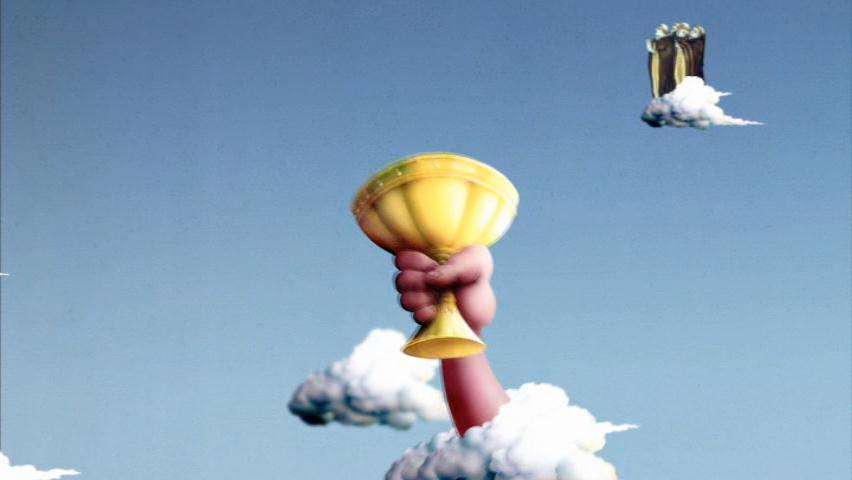
\includegraphics[width=0.8\textwidth]{grail.jpg}
%   \caption[Voorbeeld figuur.]{\label{fig:grail}Voorbeeld van invoegen van een figuur. Zorg altijd voor een uitgebreid bijschrift dat de figuur volledig beschrijft zonder in de tekst te moeten gaan zoeken. Vergeet ook je bronvermelding niet!}
% \end{figure}

% \begin{listing}
%   \begin{minted}{python}
%     import pandas as pd
%     import seaborn as sns

%     penguins = sns.load_dataset('penguins')
%     sns.relplot(data=penguins, x="flipper_length_mm", y="bill_length_mm", hue="species")
%   \end{minted}
%   \caption[Voorbeeld codefragment]{Voorbeeld van het invoegen van een codefragment.}
% \end{listing}

% \begin{table}
%   \centering
%   \begin{tabular}{lcr}
%     \toprule
%     \textbf{Kolom 1} & \textbf{Kolom 2} & \textbf{Kolom 3} \\
%     $\alpha$         & $\beta$          & $\gamma$         \\
%     \midrule
%     A                & 10.230           & a                \\
%     B                & 45.678           & b                \\
%     C                & 99.987           & c                \\
%     \bottomrule
%   \end{tabular}
%   \caption[Voorbeeld tabel]{\label{tab:example}Voorbeeld van een tabel.}
% \end{table}

Geautomatiseerde dataverzameling en -analyse spelen een steeds grotere rol in de professionele sportwereld, waar nauwkeurige statistieken noodzakelijk zijn voor prestatieverbetering en strategische besluitvorming. In de sport, in het bijzonder in volleybal, zorgt automatisering van statistiekenverzameling ervoor dat spelers en coaches beter inzicht krijgen in prestaties, waardoor training en wedstrijdvoorbereiding doelgerichter kunnen worden aangepakt.

\section{Belang van statistieken in de sportwereld}
Vooral technologieën zoals AI, computer vision en machine learning bieden nieuwe mogelijkheden om spelmomenten en spelersbewegingen nauwkeurig vast te leggen en te analyseren. De spelers- en matchstatistieken \autocite{Wahyuti2023} zijn van uiterst belang. Ze bieden niet alleen inzichten in de puntenregistratie van het team, maar ook in de tactische en technische aspecten van het spel. Volgens de studie is het belangrijk om een uitgebreid digitaal puntenregistratie bij te houden. Dit om fouten en verlies van gegevens, wat vaak voorkomt bij handmatige invoer, te minimaliseren. Uit onderzoek \autocite{Harabagiu2023} blijkt dat door gebruik van de statistische software Data Volley de efficiënte van een team met 6\% stijgt. De software identificeert de tekortkomingen en hierdoor kunnen individuele trainingsprogramma's opgesteld worden voor elke speler. Volgens \textcite{Ruiye2024} zijn de nauwkeurigheid en efficiëntie van de videoanalyse zeer belangrijk. Een innovatief videoanalysemodel gebaseerd op Bi-directional Long Short-Term Memory (BiLSTM) en aandachtsmechanismen behaalt een herkenningsnauwkeurigheid van meer dan 90\%.

Natuurlijk zijn er andere invloeden op de statistieken dan alleen de spelersprestaties \autocite{LopezSerrano2022}. Zo spelen volgens verschillende coaches het niveau van de tegenstander, het moment in een set, het scoreverschil, resultaat van de vorige set en het de competitieve druk een zeer grote in de analyse. Trainers pleiten ervoor dat er een geïntegreerde benadering is voor deze variabelen. Hierdoor wordt rekening gehouden met de specifieke omstandigheden van elke wedstrijd. Deze gegevens mogen niet geïsoleerd worden bekeken, maar juist in samenhang geanalyseerd. Bij verder onderzoek is het van essentieel belang dat coaches worden betrokken bij de ontwikkeling hiervan.

\section{Toepassing van kunstmatige intelligentie en data-analyse}
\textcite{Fadl2020} benadrukt het belang van moderne technologieën in de sport en hoe deze kunnen bijdragen aan het verbeteren van coachingsmethoden.

Om dit te bereiken, werd een beoordelingssysteem ontwikkeld waarmee coaches de bewegingsanalyse van spelers efficiënter kunnen uitvoeren. Dit systeem werd geëvalueerd door 200 ervaren volleybalcoaches en bleek binnen een korte tijdspanne van maximaal 15 minuten bruikbare inzichten te bieden. De methode omvatte verschillende analysecomponenten, zoals technische observatie, prestatiediagnose en trainingsinterventies, om coaches te helpen bij het plannen en optimaliseren van trainingssessies.
Uit de resultaten bleek dat AI-gestuurde bewegingsanalyse een effectief hulpmiddel is om trainers te ondersteunen bij het kwantificeren van prestaties en het identificeren van verbeterpunten.
Deze bevindingen onderstrepen hoe technologische vooruitgang kan bijdragen aan een betere trainingservaring, door coaches te voorzien van nauwkeurige en snelle analytische tools voor het verbeteren van de prestaties van hun spelers.

\textcite{Huang2023} ontwikkelen een AI-gestuurd model voor de detectie en herkenning van overtredingen in volleybal, ter vervanging van subjectieve scheidsrechtersoordelen. Het model maakt gebruik van videoverbeteringstechnologie en een combinatie van algoritmen, waaronder de wavelet-transformatie, de drie-frame verschilmethode en achtergrondsubtractie, om bewegende objecten te identificeren. De wavelet-transformatie is een techniek die signalen in verschillende frequenties analyseert en zowel tijd- als frequentiedomein-informatie biedt, wat helpt bij het extraheren van belangrijke kenmerken van bewegende objecten, zoals spelers en de bal. De drie-frame verschilmethode vergelijkt opeenvolgende frames in een video om veranderingen te detecteren, wat effectief helpt bij het identificeren van de beweging van objecten, zoals de bal en de spelers. Daarnaast wordt achtergrondsubtractie toegepast, waarbij het verschil tussen de huidige beeldinhoud en een vooraf gedefinieerd achtergrondmodel wordt berekend, zodat alleen de bewegende objecten ten opzichte van de achtergrond worden geïdentificeerd.
De verbeterde CamShift-trackingmethode, ondersteund door een Kalman-filter, optimaliseert de tracking van spelers door dynamisch de grootte en positie van zoekgebieden aan te passen op basis van de kleurverdeling van de objecten, wat zorgt voor nauwkeurige objectvolging. Bovendien wordt een Hidden Markov Model (HMM) ingezet voor de classificatie van overtredingen. Het HMM is een statistisch model dat de toestand van het spel op basis van sequentiële data analyseert en de waarschijnlijkheid van een overtreding voorspelt op basis van eerdere gedragingen en de huidige staat van het spel.
Uit experimentele resultaten blijkt dat het model een hoge herkenningsnauwkeurigheid heeft (99,76\%) en een gemiddelde foutmarge van 0,003. Hiermee biedt het een objectieve en betrouwbare methode voor scheidsrechtersbeslissingen, wat bijdraagt aan de eerlijkheid en nauwkeurigheid van arbitrage in volleybal. Dit onderzoek benadrukt de potentie van AI in sportanalyse en opent mogelijkheden voor bredere toepassingen in andere sporten.

\textcite{Liu2021} introduceren een innovatief model voor sportdata-visualisatie, het Video-based Effective Visualization Framework (VEVF). Dit model combineert kunstmatige intelligentie (AI) en big data-analyse om sportvideo's te classificeren en te analyseren, met als doel de prestaties van atleten te verbeteren en coaches en analisten van waardevolle inzichten te voorzien.
Het belang van data-visualisatie in de sportwereld wordt nogmaals benadrukt, vooral in het tijdperk van big data. Sportdata, zoals atleetprestaties, trainingsstatistieken en gezondheidsgegevens, kunnen worden gebruikt om betere spelstrategieën te ontwikkelen, blessures te verminderen en de prestaties van atleten te verbeteren. Het VEVF-model maakt gebruik van draagbare apparaten om real-time bewegingsdata van atleten te verzamelen en deze te visualiseren in een 3D-virtuele omgeving. Dit stelt coaches in staat om de prestaties van atleten beter te monitoren en toekomstige bewegingen te voorspellen.

\section{Gebruik van sensors en camera's voor dataverzameling}
Uit onderzoek van Xu \textcite{Sun2021} blijkt dat door de vooruitgang in elektronische en sensortechnologieën het mogelijk is geworden om menselijke bewegingen en spelmomenten nauwkeurig vast te leggen. In de sportwereld zijn sensoren en camera's steeds vaker te vinden op en naast het veld. Deze technologieën maken het mogelijk om realtime data te verzamelen over spelersposities, balbewegingen en spelsituaties door middel van sensoren aan de gewrichten van spelers te bevestigen. Door deze data te analyseren met behulp van AI-algoritmen kunnen coaches en analisten waardevolle inzichten verkrijgen in de prestaties en strategieën.

Het onderzoek van \textcite{Salim2024} richt zich op het optimaliseren van volleybaltraining door middle van geavanceerde sensortechnologie en data-analyse. Er wordt een innovatief platform gepresenteert dat gebruikmaakt van een drukgevoelige vloer en machine learning om zowel atleten als coaches te ondersteunen. Het systeem kan automatisch verschillende volleybalacties herkennen. Artificiële intelligentie gaat deze acties detecteren en direct feedback geven aan de spelers. Daarnaast kan het ook automatisch belangrijke speelmomenten markeren.
Naast analyse biedt het systeem ook interactieve leeromgevingen, waarbij trainingen dynamisch worden aangepast op basis van de waargenomen bewegingen van spelers. Dit wordt mogelijk gemaakt door een combinatie van machine learning-modellen, waaronder convolutionele neurale netwerken (CNN) en actieve datarepresentatie (ADR). Convolutionele neurale netwerken vormen een klasse van diepe neurale netwerken die bijzonder geschikt zijn voor de verwerking en analyse van visuele gegevens. Ze bootsen de werking van het menselijk visuele systeem na door gebruik te maken van convolutielagen, waarbij kleine filters of kernels over een afbeelding schuiven om patronen en kenmerken zoals randen, vormen en texturen te detecteren. Dit maakt CNN's zeer effectief voor taken zoals beeldherkenning, objectdetectie en actieclassificatie, wat cruciaal is in interactieve leeromgevingen waarbij spelersbewegingen worden geanalyseerd en gebruikt om trainingen dynamisch aan te passen. Deze technologieën behaalden een nauwkeurigheid tot 78,71\% bij het herkennen van acties.
Deze technologie heeft wel nog verdere verbeteringen nodig vooraleer het in de praktijk kan toegepast worden, maar het toont wel aan dat de manier waarop volleybaltrainingen vorm krijgen fundamenteel kunnen veranderen.

\textcite{Liang2023} concludeerden dat traditionele videoanalysemethode vaak te beperkt is voor de variabele omstandigheden zoals verlichting en achtergrond tijdens het spel. Skeletdata biedt hier een oplossing voor door de bewegingen van spelers te vereenvoudigen tot een netwerk van verbonden gewrichten. De complexiteit van de visuele gegevens vermindert hierdoor. De methode zou nog een extra assistentie kunnen bieden aan de coaches en spelers.

\section{Gebruik van machine learning voor analyse van volleybaldata}
De integratie van machine learning en digitale informatietechnologie in volleybal biedt nieuwe mogelijkheden voor prestatieverbetering en spelanalyse.

\textcite{Musa2021} onderzoeken welke factoren bijdragen aan het identificeren van getalenteerde volleybalspelers. Hierbij werd gekeken naar zowel fysieke kenmerken, zoals lengte, gewicht en leeftijd, als psychologische aspecten, waaronder mentale weerbaarheid en voorbereiding op wedstrijden. Door middel van machine learning werden spelers ingedeeld in twee prestatiecategorieën: hoogpresterend (HVP) en laagpresterend (LVP).
Uit de resultaten bleek dat gewicht, leeftijd en psychologische vaardigheden significante verschillen vertoonden tussen de twee groepen, terwijl lengte geen doorslaggevende factor was. Hoogpresterende spelers blonken vooral uit in mentale strategieën zoals zelfspraak, visualisatie en emotieregulatie, wat een belangrijke rol bleek te spelen bij succes op het veld.
Deze studie benadrukt het belang van zowel fysieke als mentale factoren bij het selecteren van talentvolle volleybalspelers. Daarnaast laat het zien hoe machine learning kan worden ingezet als hulpmiddel voor coaches bij het scouten en samenstellen van teams.

Het onderzoek van \textcite{Dai2021} richt zich op het gebruik van machine learning voor de analyse van volleybaldata. Het doel is om spelers en coaches meer inzicht te geven in de technische uitvoering van bewegingen, met name de smash zoals afgebeeld in figuur \ref{fig:spike} en de bijbehorende spieractiviteit. In het experiment werden twaalf volleybalspelers onderverdeeld in twee groepen: één groep gebruikte een preswing-techniek met beide armen (type A), terwijl de andere groep deze techniek niet toepaste (type B).
Door middel van kinematische, dynamische en elektromyografische analyses werden de verschillende fasen van de smash bestudeerd, van de aanloop en afzet tot het moment van raken. De resultaten toonden aan dat type A-spelers over het algemeen een betere balans hadden in spieractiviteit tussen beide zijden van het lichaam. Bij type B-spelers werd daarentegen een grotere afhankelijkheid van de beenspieren vastgesteld, wat suggereert dat zij compenseren voor het ontbreken van een preswing-beweging met de armen.
Daarnaast bleek dat de kracht die tijdens de sprong werd gegenereerd, bij type A hoger was dan bij type B, wat duidt op een efficiëntere energieoverdracht. Ook was er een verschil in de bijdrage van de rompspieren, waarbij de rechte buikspier bij type A een evenwichtige rol speelde, terwijl deze bij type B een dominante functie had.

\begin{figure}
  \centering
  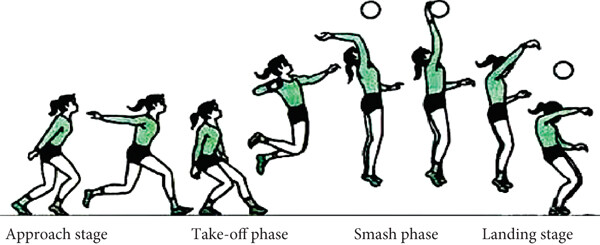
\includegraphics[width=0.8\textwidth]{spike.jpg}
  \caption{\label{fig:spike}Een reeks actiediagrammen van volleybal-spikes.}
  \autocite{Dai2021}
\end{figure}

Machine learning kan ook worden ingezet om blessures bij professionele volleyballers te monitoren en te voorspellen, volgens \textcite{Leeuw2021}. Door dagelijks gegevens te verzamelen over trainingsbelasting, sprongbelasting en welzijnsindicatoren, probeerden de onderzoekers inzicht te krijgen in het ontstaan en de ontwikkeling van overbelastingsblessures.
Voor dit onderzoek werden veertien topspelers gedurende 24 weken gevolgd. Ze vulden dagelijks vragenlijsten in over hun fysieke toestand en blessures, terwijl hun fysieke activiteiten en sprongbelasting werden geregistreerd via draagbare sensoren. De gegevens werden geanalyseerd met de machine learning-techniek Subgroup Discovery, waarmee verbanden tussen trainingsbelasting, welzijn en blessurerisico per individuele speler werden geïdentificeerd.
Uit de resultaten bleek dat verhoogde sprongbelasting een belangrijke voorspeller was van overbelastingsblessures, vooral aan de knieën. Daarnaast verschilden de risicofactoren per speler, wat het belang van een gepersonaliseerde aanpak onderstreept. Door patronen te herkennen in trainingsbelasting en blessureklachten, konden de onderzoekers gepersonaliseerd advies formuleren om blessures te helpen voorkomen.

\textcite{Yu2022} verkennen hoe kunstmatige neurale netwerken en genetische algoritmen kunnen bijdragen aan een betere beoordeling van serveer-, landings- en blokkeeracties. Door deze technologieën toe te passen, wordt niet alleen de reactietijd van spelers verbeterd, maar neemt ook de nauwkeurigheid van beslissingen toe, wat essentieel is voor training en blessurepreventie.
Verder worden clustering, regressieanalyse en informatieverwerking gebruikt om patronen in spelprestaties te identificeren en te voorspellen. De bevindingen tonen aan dat spelers met een hoger vaardigheidsniveau efficiënter tactische informatie verwerken en sneller reageren op speelsituaties. Dit onderzoek onderstreept de potentie van AI-gebaseerde technologieën in de sportwetenschap en biedt waardevolle inzichten voor coaching en prestatieanalyse.

\section{Bestaande AI-systemen voor sportstatistieken}
Er zijn verschillende AI-systemen beschikbaar die kunnen worden ingezet voor het verzamelen en analyseren van sportstatistieken. In tabel \ref{tab:tools} worden ze vergeleken met DataVolley, de tool die momenteel wordt gebruikt.

\begin{table}
  \centering
  \begin{tabular}{lcr}
    \toprule
    \textbf{Tool} & \textbf{Real-time} & \textbf{Video-input}\\
    \midrule
    DataVolley & Ja & Handmatige invoer \\
    Balltime AI & Nee & Opgenomen of live \\
    Volleymetrics & Nee & Opgenomen \\
    SportsVisio & Nee & Opgenomen of live \\
    SmashVision & Ja & Opgenomen of live \\
    \bottomrule
  \end{tabular}
  \caption[Korte vergelijking bestaande tools]{\label{tab:tools}Korte vergelijking bestaande tools}
\end{table}

Bij de analyse van volleybalwedstrijden en -trainingen worden verschillende tools ingezet om speldata te verzamelen en te verwerken. Deze tools verschillen op twee belangrijke aspecten: real-time verwerking en de wijze van video-input.

Sommige tools bieden real-time analyse, wat betekent dat gegevens direct tijdens de wedstrijd of training verwerkt en geanalyseerd worden. Dit is het geval bij Balltime AI en SportsVisio. Andere tools, zoals DataVolley en VolleyMetrics, bieden deze mogelijkheid niet en verwerken gegevens pas achteraf op basis van opgenomen videobeelden of handmatige invoer.

Naast real-time verwerking verschilt ook de manier waarop videobeelden worden gebruikt. DataVolley vereist een handmatige invoer van data met videobeelden, terwijl VolleyMetrics uitsluitend werkt met opgenomen video’s. De andere tools, zoals Balltime AI, Hudl Volleyball en SportsVisio, kunnen zowel opgenomen als live beelden verwerken. Dit maakt deze tools flexibeler in hun toepassing, omdat ze zowel achteraf als tijdens de wedstrijd analyses kunnen leveren.

De keuze voor een bepaalde analysetool hangt af van de specifieke behoeften van de gebruiker. Indien directe feedback gewenst is, zijn tools met real-time verwerking geschikter. Voor diepgaande analyse op basis van bestaande beelden kunnen niet-real-time tools een waardevolle aanvulling zijn.
%%=============================================================================
%% Methodologie
%%=============================================================================

\chapter{\IfLanguageName{dutch}{Methodologie}{Methodology}}%
\label{ch:methodologie}

%% In dit hoofstuk geef je een korte toelichting over hoe je te werk bent
%% gegaan. Verdeel je onderzoek in grote fasen, en licht in elke fase toe wat
%% de doelstelling was, welke deliverables daar uit gekomen zijn, en welke
%% onderzoeksmethoden je daarbij toegepast hebt. Verantwoord waarom je
%% op deze manier te werk gegaan bent.
%% 
%% Voorbeelden van zulke fasen zijn: literatuurstudie, opstellen van een
%% requirements-analyse, opstellen long-list (bij vergelijkende studie),
%% selectie van geschikte tools (bij vergelijkende studie, "short-list"),
%% opzetten testopstelling/PoC, uitvoeren testen en verzamelen
%% van resultaten, analyse van resultaten, ...
%%
%% !!!!! LET OP !!!!!
%%
%% Het is uitdrukkelijk NIET de bedoeling dat je het grootste deel van de corpus
%% van je bachelorproef in dit hoofstuk verwerkt! Dit hoofdstuk is eerder een
%% kort overzicht van je plan van aanpak.
%%
%% Maak voor elke fase (behalve het literatuuronderzoek) een NIEUW HOOFDSTUK aan
%% en geef het een gepaste titel.


\subsection{Fase 1: Literatuurstudie}
De literatuurstudie is bedoeld om inzicht te krijgen in de huidige stand van zaken met betrekking tot AI-systemen die geschikt zijn voor het verzamelen en analyseren van sportstatistieken. Ook wordt gekeken naar AI-modellen die in recent onderzoek effectief bleken voor sportanalyse. Daarnaast wordt ook de rol van sensors en camera's onderzocht. Waarom zijn statistieken belangrijk in de sportwereld en specifiek in volleybal? Deze vraag wordt beantwoord door het analyseren van academische publicaties en praktijkvoorbeelden. Daarnaast worden whitepapers en technische documentatie van bekende AI-tools, zoals Hudl, DataVolley, Second Spectrum en Balltime AI, bestudeerd.

De focus ligt hierbij op het beoordelen van nauwkeurigheid, snelheid, schaalbaarheid en kosten van deze systemen, omdat deze factoren belangrijk zijn voor de toepassing binnen Lindemans Aalst. Welke technologieën worden momenteel gebruikt voor het automatiseren van sportstatistieken? Dit wordt onderzocht door een overzicht te creëren van bestaande systemen en technologieën.

Aan het einde van deze fase wordt een overzichtsrapport opgesteld met de bevindingen, waarin ook een vergelijkingstabel wordt opgenomen die de sterke en zwakke punten van elk systeem schetst. Dit rapport vormt de basis voor de selectie van systemen die in latere fases verder onderzocht zullen worden.
\subsection{Fase 2: Interviews en requirementsanalyse}
In de tweede fase worden gestructureerde interviews afgenomen met de coaches, data-analisten en technische staf van Lindemans Aalst. Het doel van deze interviews is om een duidelijk beeld te krijgen van de functionele en technische eisen die de club stelt aan een geautomatiseerd statistieken systeem. Daarnaast wordt onderzocht in hoeverre de technische staf en spelers bereid zijn AI-technologie te omarmen en welke barrières er zijn bij implementatie. Ook wordt extra aandacht besteed aan de gebruiksvriendelijkheid van de systemen en de mate van benodigde technische kennis bij gebruikers. "Hoe presteren bestaande AI-systemen voor het verzamelen en analyseren van volleybalstatistieken?" en "Welke technologieën worden momenteel gebruikt voor het automatiseren van sportstatistieken?". Deze vragen worden besproken met stakeholders, waarbij hun ervaringen en verwachtingen worden genoteerd.

De requirementsanalyse richt zich op de statistieken die essentieel zijn voor de club en op specifieke analyses die coaches tijdens wedstrijden en trainingen nodig hebben. De inzichten uit deze gesprekken worden verwerkt in een requirementsdocument, dat de functionele en technische vereisten vastlegt. Dit document vormt een referentiepunt voor de vergelijkende analyse van de AI-systemen in de volgende fase.
\subsection{Fase 3: Vergelijkende studie van AI-systemen}
In deze fase worden de geselecteerde AI-systemen geëvalueerd op basis van nauwkeurigheid, snelheid en gebruiksgemak, om objectief te bepalen welke oplossing het best aansluit bij de eisen van Lindemans Aalst. Hiervoor wordt gebruikgemaakt van eerder verzamelde datasets van match- en trainingsgegevens. "Hoe presteren bestaande AI-systemen voor het verzamelen en analyseren van volleybalstatistieken?" wordt verder onderzocht door de prestaties van de systemen in de praktijk te testen en te vergelijken met handmatig geregistreerde data.

De systemen worden getest op hun vermogen om deze data nauwkeurig en snel te verwerken. Hierbij wordt niet alleen gekeken naar nauwkeurigheid en snelheid, maar ook naar de integratie met de bestaande infrastructuur van Lindemans Aalst. Daarnaast worden skeletgebaseerde AI-systemen zoals beschreven in de literatuurstudie meegenomen in de evaluatie, om hun potentieel binnen volleybalanalyse te beoordelen. De resultaten worden gepresenteerd in een rapport met grafieken en tabellen die de prestaties van elk systeem visueel weergeven. Het rapport bevat ook een concrete aanbeveling van het systeem dat het meest geschikt lijkt voor implementatie, op basis van de vergelijking.
\subsection{Fase 4: Proof of concept en praktijktest}
Na de vergelijkende studie wordt het aanbevolen systeem geïmplementeerd als proof of concept (PoC) bij Lindemans Aalst, op voorwaarde dat het seizoen nog bezig is. Deze praktijktest heeft als doel te valideren of het systeem daadwerkelijk voldoet aan de functionele en technische eisen van de club. Gedurende deze periode verzamelt het systeem automatisch gegevens tijdens trainingen en wedstrijden, zodat coaches en analisten het gebruiksgemak en de nauwkeurigheid van de automatisering kunnen evalueren. De prestaties van AI worden vergeleken met de traditionele methode om te bepalen of AI een significante meerwaarde biedt."

De prestaties van het PoC-systeem worden vergeleken met handmatig geregistreerde gegevens en de feedback van de coaches over de gebruiksvriendelijkheid wordt verzameld. Aan het einde van deze fase wordt een validatierapport opgesteld, waarin de kwantitatieve resultaten van het geautomatiseerde systeem zijn opgenomen, evenals eventuele aanbevelingen voor optimalisatie.
\subsection{Fase 5: Analyse en eindrapport}
In de laatste fase worden de resultaten van het onderzoek geanalyseerd en samengebracht in een eindrapport. Dit rapport bevat een grondige analyse van de prestaties van het PoC-systeem en conclusies over de mate waarin het systeem de doelstellingen van Lindemans Aalst ondersteunt. "Waarom zijn statistieken belangrijk in de sportwereld en specifiek in volleybal?" wordt in deze fase opnieuw geëvalueerd op basis van de praktische resultaten.

De data uit de eerdere fases worden statistisch geanalyseerd om objectieve conclusies te trekken over de invloed van automatisering op de nauwkeurigheid en snelheid van statistiekenregistratie. Het rapport bevat zowel aanbevelingen voor de club over de definitieve implementatie van het AI-systeem als suggesties voor toekomstige optimalisaties.


% Voeg hier je eigen hoofdstukken toe die de ``corpus'' van je bachelorproef
% vormen. De structuur en titels hangen af van je eigen onderzoek. Je kan bv.
% elke fase in je onderzoek in een apart hoofdstuk bespreken.

%\input{...}
%\input{...}
%...
\chapter{\IfLanguageName{dutch}{Interviews en requirementsanalyse}{Interviews and requirement analysis}}%
\label{ch:interviews}

In dit hoofdstuk worden de resultaten besproken van de interviews met de technische staf en bestuur van Lindemans Aalst. Het doel is om de functionele en technische eisen in kaart te brengen die de club stelt aan een geautomatiseerd statistisch analysesysteem. De inzichten uit deze gesprekken vormen de basis voor een requirementsdocument, dat op zijn beurt dient als uitgangspunt voor de vergelijkende analyse van AI-systemen in de volgende fase.

De vragen zijn gestructureerd rond vier kernonderwerpen: functionele en technische eisen, gebruik van AI en automatisering, barrières en implementatie-uitdagingen en gebruiksvriendelijkheid en toegankelijkheid. Het is belangrijk te vermelden dat niet iedereen elke vraag kreeg. Per functie werden de juiste vragen gesteld, zodat de antwoorden specifiek aansluiten bij de rol en verantwoordelijkheid van de geïnterviewde.

Door deze gestructureerde aanpak wordt een helder beeld geschetst van de verwachtingen en behoeften van de technische staf, wat cruciaal is voor de verdere ontwikkeling en selectie van een geschikt AI-ondersteund statistisch systeem.

\section{Inzichten van stakeholders}

\subsection{Functionele en technische eisen}
\begin{enumerate}
  \item Welke statistieken zijn voor jullie het belangrijkst bij het analyseren van wedstrijden en trainingen?
  \subsubsection{Interview met de coach}
  Bij de analyse van wedstrijden en de scouting van tegenstanders worden verschillende prestatie-indicatoren geëvalueerd. Belangrijke factoren zijn de scoringspercentages in side-out en transitie, de gemaakte fouten en de rotaties waarin deze het meest voorkomen. Daarnaast wordt geanalyseerd in welke rotaties de tegenstander het meest effectief is en welke spelers in specifieke situaties het vaakst worden aangespeeld.

  De rol van de setter is hierbij essentieel. Er wordt onderzocht welke keuzes hij maakt in verschillende recepties en rotaties en in welke posities de tegenstander het hoogste scoringspercentage behaalt. Verder wordt gekeken naar de richtingen van de aanvallers, de verdedigingspatronen en de servicevariaties.
  
  Bij de vergelijking met het eigen team ligt de focus vooral op de receptie. Hierbij wordt geanalyseerd hoe spelers de service verwerken (links, rechts, boven- of onderhands) en of er zwakke punten zijn, zoals moeite met korte of diepe ballen of een voorkeur voor een specifieke kant. Deze informatie helpt om strategieën te optimaliseren en het eigen spel te verbeteren.
  \subsubsection{Interview met de assistent-coach}
  Bij de analyse van een team worden zowel de scoringpercentages uit side-out als uit transitie (wanneer de rally bezig is) bekeken. Dit gebeurt zowel op groepsniveau als per rotatie, zodat we inzicht krijgen in welke rotaties moeilijker of makkelijker zijn voor het team. Het is van belang om te weten waar de sterke en zwakke plekken per rotatie liggen.

  Daarnaast worden de individuele prestaties van spelers geanalyseerd, zowel in termen van wiskundige scores als in hun bijdrage aan het team. De verdeling van de setter wordt nauwkeurig geobserveerd, waarbij gekeken wordt of hij bepaalde spelers vaker of minder vaak aanspeelt. Het kan opvallen of een speler minder vaak wordt aangespeeld, wat mogelijk wijst op een specifieke tactiek of voorkeur van de setter.

  Bij de tegenstander wordt eenzelfde analyse uitgevoerd, maar hier ligt de nadruk minder op individuele percentages, tenzij een speler uitblinkt met slechte cijfers in receptie. Dit is belangrijk om te begrijpen of een bepaalde speler mogelijk meer ballen ontvangt, ondanks een zwakke receptie en hoe dit de tegenstander beïnvloedt.

  Door deze gegevens kunnen we inschatten wie de grootste kans heeft om de pas te krijgen per rotatie en hoe de tegenstander zijn setter verdeelt. Dit helpt bij het bepalen van strategische aanpassingen en het identificeren van zwakke plekken in de verdediging van zowel ons eigen team als dat van de tegenstander.
  \subsubsection{Interview met de scouter}
  Tijdens de trainingen ligt de nadruk vooral op opslag en receptie. Voor wedstrijden wordt de analyse uitgebreider. Naast opslag en receptie, wordt er ook gekeken naar de receptie van de tegenpartij, het spelgedrag van hun setter en de aanvalsrichtingen. 
  \item Welke data wordt momenteel handmatig verzameld en welke processen zouden jullie willen automatiseren?
  \subsubsection{Interview met de coach}
  Scouting wordt steeds verder geautomatiseerd, waarbij data-invoer leidt tot automatische analyses, zoals de aanvalsrichtingen van spelers en de settercalls. Als de scouting goed wordt uitgevoerd, biedt dit direct inzicht in de verdedigingspatronen en aanvalsvoorkeuren van de tegenstander.

  Hoewel automatisering veel werk uit handen neemt, blijft videobeelden analyseren een belangrijk voordeel. Hiermee kunnen specifieke patronen, zoals de aanvalsrichting van een speler, duidelijk worden geïdentificeerd. Scoutingsoftware en analysesystemen zorgen ervoor dat veel werk al vooraf wordt gedaan, waardoor de rol van handmatige scouting steeds kleiner wordt.

  Als technologie zich verder ontwikkelt, zou scouting op termijn mogelijk volledig geautomatiseerd kunnen worden. Dit zou het proces efficiënter maken en de behoefte aan traditionele scouts verminderen.
  \subsubsection{Interview met de assistent-coach}
  De data wordt ingevoerd door de scouter en omvat gedetailleerde informatie over de receptie van de spelers, zoals of ze voor, achter, links of rechts van zich de bal ontvangen. Het proces begint al bij de opslag: waar de opslag vandaan komt en waar de bal naartoe gaat, gevolgd door een analyse van de receptie en waar de speler de bal heeft ontvangen. Deze gedetailleerde informatie biedt een helder beeld van hoe goed een speler presteert in verschillende situaties.

  Met deze gegevens kun je de serve aanpassen en gericht kiezen welk doelwit je probeert te bereiken, afhankelijk van de sterkte en zwaktes van de tegenstander. De scouter levert dus een cruciale hoeveelheid informatie, die, als deze automatisch zou kunnen worden verzameld, ideaal zou zijn.

  Als het mogelijk is om de basis van deze gegevens geautomatiseerd te ontvangen, zou dat al een enorme vooruitgang zijn. Dit maakt het mogelijk om snel met de gegevens aan de slag te gaan, zelfs tijdens een training, zonder dat er een scouter nodig is. Het geautomatiseerd verkrijgen van deze informatie zou het proces veel efficiënter maken en stelt het team in staat om sneller en effectiever te analyseren en aan te passen.
  \subsubsection{Interview met de scouter}
  Alle wedstrijd- en trainingsdata wordt zorgvuldig ingevoerd, waarna er via specifieke worksheets (afgeleiden van Excel in DataVolley )automatisch verschillende resultaten en inzichten kunnen worden gegenereerd. Deze worksheets vormen een krachtige tool om diepgaande analyses te maken, op voorwaarde dat alle input correct is.

  Hoewel deze aanpak veel gegevens oplevert, is de gebruiksvriendelijkheid van de worksheets eerder beperkt. Momenteel moeten meerdere afzonderlijke bestanden telkens handmatig worden gedownload.

  Het zou daarom een grote meerwaarde zijn als er één centrale knop beschikbaar was waarmee alle benodigde worksheets tegelijk kunnen worden geëxporteerd. 
  \item Hoe gedetailleerd moeten de statistieken zijn? Zijn er specifieke metrics die momenteel ontbreken?
  \subsubsection{Interview met de coach}
  Hoewel scouting steeds meer wordt geautomatiseerd, zullen er altijd fouten blijven bestaan. De kwaliteit van de data hangt sterk af van de vaardigheden en ervaring van de scouter. Een goede scouter verzamelt nauwkeurigere en gedetailleerdere informatie dan iemand zonder expertise.

  Het gebruik van één programma kan het aantal fouten verminderen, maar het blijft noodzakelijk om de gegevens te controleren en te vergelijken met de invoer van de huidige scouter. Door deze vergelijking kan worden bepaald in hoeverre de data betrouwbaar is en waar eventuele correcties nodig zijn.
  \subsubsection{Interview met de assistent-coach}
  Zo gedetailleerd mogelijk. Als het minder is, zou dit weinig voordeel opleveren. Het doel is om de data zo volledig mogelijk te hebben, zodat er geen belangrijke informatie verloren gaat. Dit helpt bij het maken van betere analyses en strategische beslissingen.

  DataVolley geeft een goed overzicht van alle statistieken. Soms zijn er wat technische fouten bij dit systeem zodat er niet kan samen gewerkt worden met de scouter. Ook de kwaliteit van de internetverbinding speelt een rol voor de samenwerking.
  \item Welke outputformaten (dashboards, rapporten, live feedback) zijn het meest bruikbaar voor de technische staf?
  \subsubsection{Interview met de coach}
  Scoutinggegevens geven inzicht in verschillende spelaspecten, zoals aanvalsrichtingen en de verdeling van de setter onder verschillende omstandigheden (goede, minder goede en slechte situaties, evenals transitie). Deze informatie wordt niet alleen voorafgaand aan de wedstrijd geanalyseerd, maar ook tijdens de wedstrijd gebruikt om aanpassingen te maken.

  Tijdens de wedstrijd wordt onder andere gekeken naar servicepatronen en targets. Dit helpt bij het bepalen of er verschuivingen nodig zijn in de verdediging. Scouters zoals Joost en Erwin leveren deze informatie aan, samen met match- en setrapporten waarin wordt geanalyseerd welke patronen het meest zijn gespeeld. Deze gegevens vormen de basis voor verdere tactische beslissingen.
  \subsubsection{Interview met de assistent-coach}
  Het is belangrijk dat het snel en eenvoudig toegankelijk is. De leesbaarheid is ook belangrijk. Het is ook belangrijk dat de software op alle mogelijke computersystemen kan werken.
  \item Hoe vaak moeten de statistieken bijgewerkt worden? Is real-time verwerking gewenst?
  \subsubsection{Interview met de coach}
  Real-time scouting is vooral tijdens de wedstrijd gewenst, idealiter zelfs binnen een set. Dit kan waardevolle inzichten opleveren, maar door het hoge tempo van het spel is het niet altijd even bruikbaar. Snelle analyses kunnen helpen bij tactische aanpassingen, maar de beperkte tijd maakt het moeilijk om alles direct te verwerken en toe te passen.
  \subsubsection{Interview met de assistent-coach}
  Dit moet real-time zijn. Ten alle tijden moet de percentages van de spelers bekend zijn. Dit is belangrijk voor de coach en de spelers. De coach kan dan ook sneller ingrijpen als het nodig is.
  \subsubsection{Interview met de scouter}
  De beelden en statistieken worden nu altijd direct ingegeven en ook doorgestuurd naar de assistent-coach zodat hiermee verder kan tijdens een wedstrijd. Na de wedstrijd worden ze wel nog eens nagekeken op fouten. Bij automatiseren is dit ook nodig.
\end{enumerate}

\subsection{Gebruik van AI en automatisering}
\begin{enumerate}
  \item Welke technologieën gebruiken jullie momenteel voor statistieken en videoanalyse?
  \subsubsection{Interview met de assistent-coach}
  Momenteel wordt DataVolley gebruikt voor de statistieken. Volgend seizoen zouden we ook VolleyMetrics willen gebruiken. Dit systeem zorgt ervoor dat spelers hun eigen data kunnen bekijken, maar ook die van de tegenstander van thuis uit. Dit is belangrijk voor de spelers, omdat ze dan ook zelf kunnen zien hoe ze presteren en waar ze op moeten letten tijdens de volgende match.
  \subsubsection{Interview met de scouter}
  Er wordt momenteel gebruik gemaakt van DataVolley. Dit softwarepakket biedt mogelijkheden om videomontages en analyse te maken. VolleyMetrics gebruiken we ook voor wedstrijden waar we geen statistieken over hebben. Dit is een databank waar alle wedstrijden worden ingegeven. Het is een lostaand pakket van DataVolley. Bij dit pakket kan er per speler alle acties bekeken worden tot op de seconde. 
  \item Wat zijn de grootste voordelen en nadelen van de huidige systemen?
  \subsubsection{Interview met de assistent-coach}
  De nadelen zijn dat het niet automatisch is. Als de scouter niet aanwezig is, kan er geen data verzameld worden. De foutenlast van de andere scouter is niet geweten. De scouter geeft zelf de data in en bepaalt zelf hoe goed of slecht de speler speelt. De interpretatie is altijd anders. De data van de andere ploeg wordt eerst nog nagekeken op fouten, sommige worden niet gecorrigeerd. Dit kan leiden tot een verkeerde analyse van de tegenstander.
  \subsubsection{Interview met de scouter}
  Het grootste nadeel van het huidige systeem is dat iedereen op zijn eigen manier scout en acties beoordeelt. Het niveau tussen scouters speelt ook een grote rol. Bij een lager niveau zal er minder detail aanwezig zijn in de statistieken. Dit allemaal kan leiden tot inconsistentie in de gegevens en een gebrek aan uniformiteit in de analyses. Het is belangrijk dat alle scouts dezelfde criteria hanteren bij het invoeren van gegevens, zodat de resultaten betrouwbaar en vergelijkbaar zijn.
  \item In hoeverre staan de club open voor het gebruik van AI bij data-analyse?
  \subsubsection{Interview met de manager}
  De club staat zeker open voor nieuwe technologieën die kunnen helpen, zolang ze bijdragen aan betere prestaties. Een belangrijke factor blijft echter de kosten. De investering moet opwegen tegen de meerwaarde die het biedt. Het idee om zulke tools vanuit de liga overkoepelend verplicht te stellen, lijkt een goede benadering. Een testfase bij bepaalde clubs zou waardevolle inzichten opleveren, waarna het systeem breder geïmplementeerd kan worden, zodat alle teams er uiteindelijk van kunnen profiteren.
  \item Hebben jullie eerder ervaring met AI-gestuurde sportstatistieken? Zo ja, hoe waren die ervaringen?
  \subsubsection{Interview met de coach}
  Er is geen ervaring met AI-gestuurde sportstatistieken.
  \subsubsection{Interview met de assistent-coach}
  Er is geen ervaring met AI-gestuurde sportstatistieken.
  \subsubsection{Interview met de scouter}
  Er is geen ervaring met AI-gestuurde sportstatistieken.
  \subsubsection{Interview met de manager}
  Er is geen ervaring met AI-gestuurde sportstatistieken.
  \item Welke taken zouden jullie het liefst volledig geautomatiseerd zien?
  \subsubsection{Interview met de coach}
  Richtingen van aanvallers en de beslissingen van de setter tijdens wedstrijden is wel belangrijk. Daar kan echt beslissingen op gebasseerd worden. 
  \subsubsection{Interview met de assistent-coach}
  Het zou ideaal zijn als er bepaalde functies automatisch uitgevoerd kunnen worden. Momenteel staan die functies ook in DataVolley, maar die moeten handmatig uitgevoerd worden.
  \subsubsection{Interview met de scouter}
  De kleine zaken zoals het automatiseren van het downloaden van de worksheets zou al heel gemakkelijk zijn. De interpretaties uit de analyses zou ook automatisch kunnen gebeuren, dat AI bijvoorbeeld alle kenmerkenden zaken eruit kan halen. Als een setter bijvoorbeeld altijd naar dezelfde speler speelt of uit receptie dat er met een bepaalde zekerheid die actie zal volgen, zou dit automatisch kunnen worden opgemerkt. 
  \subsubsection{Interview met de manager}
  Het zou ideaal zijn als het scoutingproces volledig geautomatiseerd is, zodat gegevens direct en zonder handmatige invoer beschikbaar zijn. Dit zou niet alleen de efficiëntie verbeteren, maar ook personeelskosten besparen, aangezien minder tijd besteed hoeft te worden aan handmatige data-invoer en analyse. Een systeem dat automatisch de juiste informatie verzamelt en verwerkt, maakt het voor clubs gemakkelijker om snel en effectief te reageren zonder extra middelen te moeten inzetten.
\end{enumerate}


\subsection{Barrières en implementatie-uitdagingen}
\begin{enumerate}
  \item Wat zijn de grootste uitdagingen bij het implementeren van nieuwe technologieën in jullie workflow?
  \subsubsection{Interview met de coach}
  Er is openheid voor nieuwe scoutingmethodes, maar een solide basiskennis blijft essentieel. Een belangrijk vergelijkingspunt is hoe de nieuwe methode zich verhoudt tot bestaande systemen zoals DataVolley. Als een nieuw systeem al goed ontwikkeld is en vroeg kan worden geïmplementeerd, zullen er waarschijnlijk weinig problemen optreden. Dit maakt snelle aanpassingen mogelijk. Uiteindelijk moet het systeem een verbetering zijn ten opzichte van de huidige werkwijze om effectief ingezet te worden.
  \subsubsection{Interview met de assistent-coach}
  Er moet op het systeem vertrouwd kunnen worden. De data die nu verkregen wordt door de scouter moet identiek zijn aan die dat het systeem geeft. Ook de prijs van het systeem is een uitdaging. Als de AI perfect doet wat er wordt verwacht, maar de prijs is te hoog zal dit niet worden geïmplementeerd. Op training kan er dan gekeken worden naar een goedkopere oplossing, maar voor op een match is dit absoluut niet mogelijk.
  \subsubsection{Interview met de scouter}
  Tijd en kennis is hierbij wel de grootste uitdaging. De tijd die nodig is om het systeem te leren kennen en de kennis om het goed te gebruiken. Het is belangrijk dat de scouter goed weet hoe het systeem werkt, zodat het optimaal kan benut worden. Dit kan enige tijd in beslag nemen, maar is cruciaal voor een succesvolle implementatie.
  \subsubsection{Interview met de manager}
  Een belangrijk aandachtspunt bij het implementeren van geautomatiseerde systemen is de betrouwbaarheid, vooral tijdens wedstrijden. Aangezien de club veel met vrijwilligers werkt die niet altijd de technische kennis hebben om problemen op te lossen, kan een technisch probleem (zoals het uitvallen van het systeem) tijdens een match grote gevolgen hebben, omdat er dan geen statistieken meer beschikbaar zijn. Om dit te voorkomen, zou het handig zijn om een persoon met een technische achtergrond aan te stellen die in geval van problemen snel kan ingrijpen en de benodigde ondersteuning biedt. Dit garandeert dat het systeem soepel blijft draaien en de scoutingdata op cruciale momenten toegankelijk blijft.
  \item Is er weerstand binnen de club tegen het gebruik van AI voor statistieken? Waarom wel/niet?
  \subsubsection{Interview met de manager}
  Er is geen weerstand tegen het gebruik van AI voor statistieken, zolang het systeem betrouwbaar is en de kosten in verhouding staan tot de voordelen. De club staat open voor nieuwe technologieën die kunnen helpen bij het verbeteren van prestaties en scoutingprocessen.
  \item Hoeveel technische kennis is er binnen de staf aanwezig voor het werken met geavanceerde analysesystemen?
  \subsubsection{Interview met de coach}
  Er is een vrij grote technische kennis aanwezig bij de sportieve staf.
  \subsubsection{Interview met de assistent-coach}
  Er is een vrij grote technische kennis aanwezig bij de sportieve staf.
  \subsubsection{Interview met de scouter}
  Er is een vrij grote technische kennis aanwezig bij de sportieve staf, maar er is wel genoeg tijd nodig om het systeem goed te leren kennen en te weten wat er precies mee kan gedaan worden.
  \subsubsection{Interview met de manager}
  De club heeft een aantal mensen met technische kennis, maar het is belangrijk dat deze kennis ook beschikbaar is voor de vrijwilligers die met het systeem werken. Dit kan door training of ondersteuning te bieden aan de vrijwilligers, zodat zij ook in staat zijn om het systeem effectief te gebruiken en eventuele problemen op te lossen.

  Daarnaast zou het nuttig zijn om bij het opbouwen van de zaal altijd iemand met technische expertise aanwezig te hebben. Deze persoon kan ervoor zorgen dat alles correct wordt ingesteld en goed functioneert, zodat er geen technische problemen ontstaan die het verzamelen van statistieken tijdens de wedstrijd kunnen verstoren.
  \item Welke ondersteuning of training zou nodig zijn om het systeem optimaal te benutten?
  \subsubsection{Interview met de scouter}
  Opleidingen zullen heel belangrijk zijn. Er zullen waarschijnlijk meerdere sessies nodig zijn om het systeem optimaal te kunnen benutten.
  \subsubsection{Interview met de manager}
  Om ervoor te zorgen dat alle vrijwilligers effectief met het systeem kunnen werken, is het belangrijk om meerdere trainingssessies aan te bieden. Dit helpt niet alleen om de kennis te verspreiden, maar zorgt er ook voor dat iedereen vertrouwd raakt met het systeem en in staat is om eventuele technische problemen op te lossen. Het is duidelijk dat niet iedereen dezelfde technische kennis heeft, dus herhalende sessies kunnen ervoor zorgen dat alle vrijwilligers op hetzelfde niveau staan en beter voorbereid zijn om het systeem optimaal te gebruiken.
  \item Zijn er specifieke privacy- of ethische bezwaren binnen de club met betrekking tot geautomatiseerde dataverzameling?
  \subsubsection{Interview met de manager}
  Er zijn geen bezwaren tegen geautomatiseerde dataverzameling. De General Data Protection Regulation (GDPR) heeft hier eigenlijk geen betrekkingen op.
\end{enumerate}

\subsection{Gebruiksvriendelijkheid en toegankelijkheid}
\begin{enumerate}
  \item Wat zijn de belangrijkste eigenschappen die een nieuw systeem gebruiksvriendelijk maken?
  \subsubsection{Interview met de scouter}
  Voor een vlotte en efficiënte uitwisseling van gegevens tussen stafleden is het belangrijk dat het systeem webgebaseerd is. Hierdoor kunnen data en analyses makkelijk gedeeld en geraadpleegd worden, onafhankelijk van plaats of toestel.

  Daarnaast zou een app een grote meerwaarde betekenen, vooral met het oog op communicatie met de assistent-coach tijdens wedstrijden. Via een app kan snel en discreet informatie worden gedeeld, zoals statistieken, observaties of tactische aanwijzingen.
  \item Hoe snel moet iemand zonder technische achtergrond met het systeem kunnen werken?
  \subsubsection{Interview met de assistent-coach}
  Het hangt af van de taak van de persoon. De coach kan terugvallen op de assistent, maar wordt erop afgerekend als hij het niet kent als het niet goed gaat. Als assistent-coach moet je er eigenlijk ook al mee kunnen werken omdat er binnen de seconde iets kunnen oproepen.
  \subsubsection{Interview met de scouter}
  Idealiter wordt gestart met het gebruik van een nieuw systeem in de aanloop naar het seizoen of tijdens de voorbereiding. Dit geeft voldoende tijd om vertrouwd te raken met de werking, vooral wanneer de betrokken persoon nog geen ervaring heeft met dergelijke tools.

  De leercurve verschilt sterk per systeem. Bij gevestigde programma’s zoals DataVolley is de instap doorgaans moeilijker, zeker wat betreft het invoeren van data. Bij nieuwere of specifiek op analyse gerichte systemen verloopt dit vaak iets gebruiksvriendelijker, waardoor de opstart sneller kan gaan.

  Voor het louter analyseren van gegevens zou een nieuwe gebruiker het systeem normaal gezien binnen een zestal maanden onder de knie moeten kunnen krijgen. Het invoeren van data vereist doorgaans meer oefening en begeleiding.
  \item Zijn er voorkeuren qua interface of visuele weergave van de data?
  \subsubsection{Interview met de coach}
  Elke vorm van informatie kan bijdragen aan betere analyses en tactische beslissingen. Hoe meer data beschikbaar is, hoe beter het team kan inspelen op verschillende spelsituaties. Alle extra inzichten, of het nu gaat om aanvalsrichtingen, servicepatronen of spelverdelingen, kunnen helpen bij het optimaliseren van de strategie. Daarom is elke aanvulling op de bestaande scouting welkom, mits deze betrouwbaar en praktisch toepasbaar is.
  \subsubsection{Interview met de assistent-coach}
  Het is belangrijk dat de interface gebruiksvriendelijk is en dat de data op een duidelijke manier wordt gepresenteerd. Dit maakt het gemakkelijker om snel de benodigde informatie te vinden en te begrijpen. Een overzichtelijke interface helpt ook om de gegevens effectief te analyseren en strategische beslissingen te nemen. Kleur codering kan ook nuttig zijn om snel belangrijke informatie te identificeren en te interpreteren.
  \subsubsection{Interview met de scouter}
  Ideaal gezien zou een systeem automatisch kunnen aanduiden wanneer er tijdens een wedstrijd iets gebeurt dat afwijkt van de verwachtingen uit de voorbereiding. Op die manier kan er snel geschakeld worden op basis van objectieve verschillen tussen wat vooraf geanalyseerd werd en wat effectief gebeurt op het veld.

  In de voorbereiding wordt een beeld opgesteld van hoe de tegenstander normaal speelt (wie de meeste ballen krijgt, wat de verdeling van de setter is, hoe ze serveren of ontvangen). Tijdens de wedstrijd kan dit soms anders zijn, maar momenteel moet daar de assistent-coach of scouter zelf actief naar op zoek gaan.

  Hoewel deze gegevens in DataVolley wel beschikbaar zijn, worden ze niet automatisch getoond of uitgelicht. Het zou een grote meerwaarde zijn mocht er een pakket bestaan waarin je je wedstrijdvoorbereiding invoert en dat dan automatisch real-time vergelijkt met de live wedstrijddata. Dit zou niet alleen tijd besparen, maar ook helpen bij het sneller en accurater bijsturen van de tactiek tijdens de match.
  \item Moet het systeem geïntegreerd kunnen worden met andere software die jullie al gebruiken?
  \subsubsection{Interview met de coach}
  Het is toch belangrijk dat iedereen met hetzelfde systeem werkt om consistentie en efficiëntie te waarborgen. Toch is er ruimte voor aanvullende tools of losse systemen, zolang ze een meerwaarde bieden. Idealiter zouden nieuwe methodes geïntegreerd kunnen worden in DataVolley, zodat alle informatie centraal blijft. Samenwerking tussen verschillende scoutingtools en systemen zou alleen maar voordelen opleveren, mits de integratie soepel verloopt en de bruikbaarheid gewaarborgd blijft.
  \subsubsection{Interview met de assistent-coach}
  Bij een integratie is er dan nog de combinatie en kan er geleidelijk aan evolueren naar een AI gestuurd systeem. Dat dan echt het vertrouwen heeft van iedereen. Voor een training zou het wel gemakkelijker zijn dat een apart systeem is. Dan is er geen nood aan de data die tijdens een match wordt geanalyseerd.
  \subsubsection{Interview met de scouter}
  Liefst wel, dat het compatibel is met DataVolley zodat de gegevens rechtstreeks kunnen geïmplementeerd worden.
  \subsubsection{Interview met de manager}
  Het delen van statistieken tussen clubs is verplicht voor een transparante en gezamenlijke benadering van scouting en wedstrijdanalyse. Daarom zou het logisch zijn dat het nieuwe systeem goed integreerbaar is met andere software, zodat gegevens naadloos gedeeld kunnen worden. Dit zorgt ervoor dat de informatie consistent blijft en dat alle betrokken clubs eenvoudig toegang hebben tot dezelfde data, wat de samenwerking en het gebruik van de scoutingtools aanzienlijk vergemakkelijkt.
  \item Hoe belangrijk is mobiele toegankelijkheid (bijv. via tablets of smartphones)?
  \subsubsection{Interview met de coach}
  Aangezien DataVolley veel wordt gebruikt, blijft het een belangrijke standaard binnen de scouting. Echter, de beperkte bruikbaarheid op tablets maakt het minder toegankelijk in sommige situaties. Een gebruiksvriendelijker en compacter systeem zou een grote verbetering zijn, vooral als het beter aansluit bij de moderne technologieën. De vooruitgang in scoutingsoftware laat zien dat er steeds efficiëntere en kleinere oplossingen mogelijk zijn, wat de praktische toepasbaarheid ten goede komt.
  \subsubsection{Interview met de assistent-coach}
  Het is belangrijk dat het systeem ook op tablets of smartphones toegankelijk is. Dit maakt het gemakkelijker om gegevens te bekijken en te analyseren. Mobiele toegankelijkheid vergroot de flexibiliteit en zorgt ervoor dat je altijd en overal toegang hebt tot belangrijke informatie.
  \subsubsection{Interview met de scouter}
  Dit is super belangrijk. Zeker in het hedendaagse volleybal.
\end{enumerate}

\chapter{\IfLanguageName{dutch}{Interviews en requirementsanalyse}{Interviews and requirement analysis}}%
\label{ch:requirementsanalyse}

In dit hoofdstuk worden de resultaten besproken van de interviews met de technische staf en bestuur van Lindemans Aalst. Het doel is om de functionele en technische eisen in kaart te brengen die de club stelt aan een geautomatiseerd statistisch analysesysteem. De inzichten uit deze gesprekken vormen de basis voor een requirementsdocument, dat op zijn beurt dient als uitgangspunt voor de vergelijkende analyse van AI-systemen in de volgende fase.

De vragen zijn gestructureerd rond vier kernonderwerpen: functionele en technische eisen, gebruik van AI en automatisering, barrières en implementatie-uitdagingen en gebruiksvriendelijkheid en toegankelijkheid. Het is belangrijk te vermelden dat niet iedereen elke vraag kreeg. Per functie werden de juiste vragen gesteld, zodat de antwoorden specifiek aansluiten bij de rol en verantwoordelijkheid van de geïnterviewde.

Door deze gestructureerde aanpak wordt een helder beeld geschetst van de verwachtingen en behoeften van de technische staf, wat cruciaal is voor de verdere ontwikkeling en selectie van een geschikt AI-ondersteund statistisch systeem.

\section{Inzichten van stakeholders}

\subsection{Functionele en technische eisen}
\begin{enumerate}
  \item Welke statistieken zijn voor jullie het belangrijkst bij het analyseren van wedstrijden en trainingen?
  \subsubsection{Interview met de coach}
  Bij de analyse van wedstrijden en de scouting van tegenstanders worden verschillende prestatie-indicatoren geëvalueerd. Belangrijke factoren zijn de scoringspercentages in side-out en transitie, de gemaakte fouten en de rotaties waarin deze het meest voorkomen. Daarnaast wordt geanalyseerd in welke rotaties de tegenstander het meest effectief is en welke spelers in specifieke situaties het vaakst worden aangespeeld.

  De rol van de setter is hierbij essentieel. Er wordt onderzocht welke keuzes hij maakt in verschillende recepties en rotaties, en in welke posities de tegenstander het hoogste scoringspercentage behaalt. Verder wordt gekeken naar de richtingen van de aanvallers, de verdedigingspatronen en de servicevariaties.
  
  Bij de vergelijking met het eigen team ligt de focus vooral op de receptie. Hierbij wordt geanalyseerd hoe spelers de service verwerken (links, rechts, boven- of onderhands) en of er zwakke punten zijn, zoals moeite met korte of diepe ballen of een voorkeur voor een specifieke kant. Deze informatie helpt om strategieën te optimaliseren en het eigen spel te verbeteren.

  \item Welke data wordt momenteel handmatig verzameld, en welke processen zouden jullie willen automatiseren?
  \subsubsection{Interview met de coach}
  Scouting wordt steeds verder geautomatiseerd, waarbij data-invoer leidt tot automatische analyses, zoals de aanvalsrichtingen van spelers en de settercalls. Als de scouting goed wordt uitgevoerd, biedt dit direct inzicht in de verdedigingspatronen en aanvalsvoorkeuren van de tegenstander.

  Hoewel automatisering veel werk uit handen neemt, blijft videobeelden analyseren een belangrijk voordeel. Hiermee kunnen specifieke patronen, zoals de aanvalsrichting van een speler, duidelijk worden geïdentificeerd. Scoutingsoftware en analysesystemen zorgen ervoor dat veel werk al vooraf wordt gedaan, waardoor de rol van handmatige scouting steeds kleiner wordt.

  Als technologie zich verder ontwikkelt, zou scouting op termijn mogelijk volledig geautomatiseerd kunnen worden. Dit zou het proces efficiënter maken en de behoefte aan traditionele scouts verminderen.
  \item Hoe gedetailleerd moeten de statistieken zijn? Zijn er specifieke metrics die momenteel ontbreken?
  \subsubsection{Interview met de coach}
  Hoewel scouting steeds meer wordt geautomatiseerd, zullen er altijd fouten blijven bestaan. De kwaliteit van de data hangt sterk af van de vaardigheden en ervaring van de scouter. Een goede scouter verzamelt nauwkeurigere en gedetailleerdere informatie dan iemand zonder expertise.

  Het gebruik van één programma kan het aantal fouten verminderen, maar het blijft noodzakelijk om de gegevens te controleren en te vergelijken met de invoer van de huidige scouter. Door deze vergelijking kan worden bepaald in hoeverre de data betrouwbaar is en waar eventuele correcties nodig zijn.
  \item Welke outputformaten (dashboards, rapporten, live feedback) zijn het meest bruikbaar voor de technische staf?
  \subsubsection{Interview met de coach}
  Scoutinggegevens geven inzicht in verschillende spelaspecten, zoals aanvalsrichtingen en de verdeling van de setter onder verschillende omstandigheden (goede, minder goede en slechte situaties, evenals transitie). Deze informatie wordt niet alleen voorafgaand aan de wedstrijd geanalyseerd, maar ook tijdens de wedstrijd gebruikt om aanpassingen te maken.

  Tijdens de wedstrijd wordt onder andere gekeken naar servicepatronen en targets. Dit helpt bij het bepalen of er verschuivingen nodig zijn in de verdediging. Scouters zoals Joost en Erwin leveren deze informatie aan, samen met match- en setrapporten waarin wordt geanalyseerd welke patronen het meest zijn gespeeld. Deze gegevens vormen de basis voor verdere tactische beslissingen.
  \item Hoe vaak moeten de statistieken bijgewerkt worden? Is real-time verwerking gewenst?
  \subsubsection{Interview met de coach}
  Real-time scouting is vooral tijdens de wedstrijd gewenst, idealiter zelfs binnen een set. Dit kan waardevolle inzichten opleveren, maar door het hoge tempo van het spel is het niet altijd even bruikbaar. Snelle analyses kunnen helpen bij tactische aanpassingen, maar de beperkte tijd maakt het moeilijk om alles direct te verwerken en toe te passen.
\end{enumerate}

\subsection{Gebruik van AI en automatisering}
\begin{enumerate}
  \item Welke technologieën gebruiken jullie momenteel voor statistieken en videoanalyse?
  \item Wat zijn de grootste voordelen en nadelen van de huidige systemen?
  \item In hoeverre staan de club open voor het gebruik van AI bij data-analyse?
  \subsubsection{Interview met de manager}
  De club staat zeker open voor nieuwe technologieën die kunnen helpen, zolang ze bijdragen aan betere prestaties. Een belangrijke factor blijft echter de kosten. De investering moet opwegen tegen de meerwaarde die het biedt. Het idee om zulke tools vanuit de liga overkoepelend verplicht te stellen, lijkt een goede benadering. Een testfase bij bepaalde clubs zou waardevolle inzichten opleveren, waarna het systeem breder geïmplementeerd kan worden, zodat alle teams er uiteindelijk van kunnen profiteren.
  \item Hebben jullie eerder ervaring met AI-gestuurde sportstatistieken? Zo ja, hoe waren die ervaringen?
  \subsubsection{Interview met de coach}
  Er is geen ervaring met AI-gestuurde sportstatistieken.
  \subsubsection{Interview met de manager}
  Er is geen ervaring met AI-gestuurde sportstatistieken.
  \item Welke taken zouden jullie het liefst volledig geautomatiseerd zien?
  \subsubsection{Interview met de coach}
  Richtingen van aanvallers en de beslissingen van de setter tijdens wedstrijden is wel belangrijk. Daar kan echt beslissingen op gebasseerd worden. 
  \subsubsection{Interview met de manager}
  Het zou ideaal zijn als het scoutingproces volledig geautomatiseerd is, zodat gegevens direct en zonder handmatige invoer beschikbaar zijn. Dit zou niet alleen de efficiëntie verbeteren, maar ook personeelskosten besparen, aangezien minder tijd besteed hoeft te worden aan handmatige data-invoer en analyse. Een systeem dat automatisch de juiste informatie verzamelt en verwerkt, maakt het voor clubs gemakkelijker om snel en effectief te reageren zonder extra middelen te moeten inzetten.
\end{enumerate}


\subsection{Barrières en implementatie-uitdagingen}
\begin{enumerate}
  \item Wat zijn de grootste uitdagingen bij het implementeren van nieuwe technologieën in jullie workflow?
  \subsubsection{Interview met de coach}
  Er is openheid voor nieuwe scoutingmethodes, maar een solide basiskennis blijft essentieel. Een belangrijk vergelijkingspunt is hoe de nieuwe methode zich verhoudt tot bestaande systemen zoals DataVolley. Als een nieuw systeem al goed ontwikkeld is en vroeg kan worden geïmplementeerd, zullen er waarschijnlijk weinig problemen optreden. Dit maakt snelle aanpassingen mogelijk. Uiteindelijk moet het systeem een verbetering zijn ten opzichte van de huidige werkwijze om effectief ingezet te worden.
  \subsubsection{Interview met de manager}
  Een belangrijk aandachtspunt bij het implementeren van geautomatiseerde systemen is de betrouwbaarheid, vooral tijdens wedstrijden. Aangezien de club veel met vrijwilligers werkt die niet altijd de technische kennis hebben om problemen op te lossen, kan een technisch probleem (zoals het uitvallen van het systeem) tijdens een match grote gevolgen hebben, omdat er dan geen statistieken meer beschikbaar zijn. Om dit te voorkomen, zou het handig zijn om een persoon met een technische achtergrond aan te stellen die in geval van problemen snel kan ingrijpen en de benodigde ondersteuning biedt. Dit garandeert dat het systeem soepel blijft draaien en de scoutingdata op cruciale momenten toegankelijk blijft.
  \item Is er weerstand binnen de club tegen het gebruik van AI voor statistieken? Waarom wel/niet?
  \subsubsection{Interview met de manager}
  Er is geen weerstand tegen het gebruik van AI voor statistieken, zolang het systeem betrouwbaar is en de kosten in verhouding staan tot de voordelen. De club staat open voor nieuwe technologieën die kunnen helpen bij het verbeteren van prestaties en scoutingprocessen.
  \item Hoeveel technische kennis is er binnen de staf aanwezig voor het werken met geavanceerde analysesystemen?
  \subsubsection{Interview met de coach}
  Er is een vrij grote technische kennis aanwezig bij de sportieve staf.
  \subsubsection{Interview met de manager}
  De club heeft een aantal mensen met technische kennis, maar het is belangrijk dat deze kennis ook beschikbaar is voor de vrijwilligers die met het systeem werken. Dit kan door training of ondersteuning te bieden aan de vrijwilligers, zodat zij ook in staat zijn om het systeem effectief te gebruiken en eventuele problemen op te lossen.

  Daarnaast zou het nuttig zijn om bij het opbouwen van de zaal altijd iemand met technische expertise aanwezig te hebben. Deze persoon kan ervoor zorgen dat alles correct wordt ingesteld en goed functioneert, zodat er geen technische problemen ontstaan die het verzamelen van statistieken tijdens de wedstrijd kunnen verstoren.
  \item Welke ondersteuning of training zou nodig zijn om het systeem optimaal te benutten?
  \subsubsection{Interview met de manager}
  Om ervoor te zorgen dat alle vrijwilligers effectief met het systeem kunnen werken, is het belangrijk om meerdere trainingssessies aan te bieden. Dit helpt niet alleen om de kennis te verspreiden, maar zorgt er ook voor dat iedereen vertrouwd raakt met het systeem en in staat is om eventuele technische problemen op te lossen. Het is duidelijk dat niet iedereen dezelfde technische kennis heeft, dus herhalende sessies kunnen ervoor zorgen dat alle vrijwilligers op hetzelfde niveau staan en beter voorbereid zijn om het systeem optimaal te gebruiken.
  \item Zijn er specifieke privacy- of ethische bezwaren binnen de club met betrekking tot geautomatiseerde dataverzameling?
  \subsubsection{Interview met de manager}
  Er zijn geen bezwaren tegen geautomatiseerde dataverzameling. De General Data Protection Regulation (GDPR) heeft hier eigenlijk geen betrekkingen op.
\end{enumerate}

\subsection{Gebruiksvriendelijkheid en toegankelijkheid}
\begin{enumerate}
  \item Wat zijn de belangrijkste eigenschappen die een nieuw systeem gebruiksvriendelijk maken?
  \item Hoe snel moet iemand zonder technische achtergrond met het systeem kunnen werken?
  \item Zijn er voorkeuren qua interface of visuele weergave van de data?
  \subsubsection{Interview met de coach}
  Elke vorm van informatie kan bijdragen aan betere analyses en tactische beslissingen. Hoe meer data beschikbaar is, hoe beter het team kan inspelen op verschillende spelsituaties. Alle extra inzichten, of het nu gaat om aanvalsrichtingen, servicepatronen of spelverdelingen, kunnen helpen bij het optimaliseren van de strategie. Daarom is elke aanvulling op de bestaande scouting welkom, mits deze betrouwbaar en praktisch toepasbaar is.
  \item Moet het systeem geïntegreerd kunnen worden met andere software die jullie al gebruiken?
  \subsubsection{Interview met de coach}
  Het is toch belangrijk dat iedereen met hetzelfde systeem werkt om consistentie en efficiëntie te waarborgen. Toch is er ruimte voor aanvullende tools of losse systemen, zolang ze een meerwaarde bieden. Idealiter zouden nieuwe methodes geïntegreerd kunnen worden in DataVolley, zodat alle informatie centraal blijft. Samenwerking tussen verschillende scoutingtools en systemen zou alleen maar voordelen opleveren, mits de integratie soepel verloopt en de bruikbaarheid gewaarborgd blijft.
  \subsubsection{Interview met de manager}
  Het delen van statistieken tussen clubs is verplicht voor een transparante en gezamenlijke benadering van scouting en wedstrijdanalyse. Daarom zou het logisch zijn dat het nieuwe systeem goed integreerbaar is met andere software, zodat gegevens naadloos gedeeld kunnen worden. Dit zorgt ervoor dat de informatie consistent blijft en dat alle betrokken clubs eenvoudig toegang hebben tot dezelfde data, wat de samenwerking en het gebruik van de scoutingtools aanzienlijk vergemakkelijkt.
  \item Hoe belangrijk is mobiele toegankelijkheid (bijv. via tablets of smartphones)?
  \subsubsection{Interview met de coach}
  Aangezien DataVolley veel wordt gebruikt, blijft het een belangrijke standaard binnen de scouting. Echter, de beperkte bruikbaarheid op tablets maakt het minder toegankelijk in sommige situaties. Een gebruiksvriendelijker en compacter systeem zou een grote verbetering zijn, vooral als het beter aansluit bij de moderne technologieën. De vooruitgang in scoutingsoftware laat zien dat er steeds efficiëntere en kleinere oplossingen mogelijk zijn, wat de praktische toepasbaarheid ten goede komt.
\end{enumerate}


\input{vergelijkendestudie}
\chapter{\IfLanguageName{dutch}{Proof of concept en praktijktest}{Proof of concept and field tests}}
\label{ch:poc}
Na de literatuurstudie, requirementsanalyse en vergelijkende evaluatie van bestaande AI-systemen, vormt dit hoofdstuk een belangrijke schakel in het beantwoorden van de centrale onderzoeksvraag. Hierin wordt het geselecteerde AI-systeem geïmplementeerd in een reële context bij volleybalclub Lindemans Aalst als een proof of concept (PoC).

Deze fase heeft tot doel om de theoretische meerwaarde van het systeem in de praktijk te valideren. Tijdens trainingen en wedstrijden wordt geëvalueerd of het systeem voldoet aan de functionele en technische vereisten zoals geformuleerd in de voorgaande fases. Hierbij wordt bijzondere aandacht besteed aan de gebruiksvriendelijkheid, de nauwkeurigheid van dataverzameling, de snelheid van verwerking en de integratie in de bestaande werkwijze van de club.

Het oorspronkelijke plan voorzag een praktijktestperiode van twee weken. Echter, aangezien het volleybalseizoen onverwacht tot een einde kwam tijdens het midden van deze fase, kon de proof of concept slechts tijdens twee resterende wedstrijden worden uitgevoerd. Ondanks deze beperkte testperiode bood dit toch waardevolle inzichten in de toepasbaarheid en prestaties van het AI-systeem in een wedstrijdcontext.

Door de prestaties van het geautomatiseerde systeem te vergelijken met handmatig geregistreerde gegevens en door feedback van coaches en staf te verzamelen, wordt nagegaan of het AI-systeem daadwerkelijk een significante meerwaarde kan bieden voor de werking van de club. De inzichten uit deze praktijktest vormen een essentiële basis voor het formuleren van aanbevelingen omtrent een bredere implementatie op lange termijn.

In bijlage \ref{ch:afkortingen} is een overzicht te vinden van de afkortingen die in dit hoofdstuk worden gebruikt. De andere statistieken en vergelijkingen zijn te vinden in bijlage \ref{ch:statistieken}.

\section{Kwartfinale Play-offs - 16/4/2025}
\subsection{Vergelijking van de statistieken}
\subsubsection{Set 2 - Lindemans Aalst}
\label{sec:PL1_Aalst2}
In de tabellen \ref{tab:PL1ServeAalstMan2} en \ref{tab:PL1ServeAalstAI2} zijn de serve statistieken van Lindemans Aalst in set 2 weergegeven. De eerste tabel toont de manueel ingevoerde statistieken, terwijl de tweede tabel de statistieken toont die door Balltime AI zijn gegenereerd. De serve statistieken zijn onderverdeeld in verschillende categorieën, zoals het aantal serves, het percentage fouten en de effectiviteit van de serve. De beoordeling van de opslag is op een andere wijze gedaan dan bij de manuele invoer. Bij de manuele invoer wordt er gebruik gemaakt van tekens, terwijl bij de AI-invoer gebruik wordt gemaakt van cijfers. Bij de opslag komt het teken \# overeen met 0, + en / met 1, ! met 2, - en = met 3. Eerst en vooral valt op dat de AI niet alle recepties heeft beoordeeld. Daarnaast kan besloten worden dat zowel de AI als de scouter de perfecte receptie gelijk beoordelen. Bij de andere vergelijking speelt de mening van de scouter een grote rol. Bij score 1 zijn er grote verschillen, enkel bij speler Max Schulz is er een zelfde hoeveelheid. Score 2 werd door de scouter niet aan een opslag gegeven, maar de AI heeft dit wel gedaan. De slechte recepties worden ook opnieuw anders beoordeeld.

\begin{table}[ht!]
  \centering
  \scriptsize
    \begin{tabular}{|l|c|c|c|c|c|c|c|c|} \hline
      \textbf{Speler} & *E\% & Tot & = & / & - & ! & + & \# \\ \hline
      Hiago Crins & 33 & 3 &  &  & 2 &  & 1 & \\ 
      Timo Lohmus & 25 & 4 & 1 &  & 1 & & 1 & 1 \\ 
      Max Schulz & 0 & 3 & 1 &  & 1 &  & 1 &  \\ 
      Mihkel Varblane & 100 & 2 &  &  &  &  & 2 & \\
      Alvaro Gimeno Rubio & 71 & 7 & 1 & 1 &  &  & 4 & 1\\
      Lucas Lorente López & 0 & 3 &  &  & 3 &  &  &  \\ \hline
  \end{tabular}
  \caption[Manueel ingevoerd opslag statistieken voor Lindemans Aalst in set 2]{\label{tab:PL1ServeAalstMan2}Manueel ingevoerd opslag statistieken voor Lindemans Aalst in set 2.}
\end{table}

\begin{table}[ht!]
  \centering
  \scriptsize
  \begin{tabular}{|l|c|c|c|c|c|c|c|c|c|c|c|c|} \hline
    \textbf{Speler} & SA & SE & TA & Pct (\%) & Eff & Rtg & 0 & 1 & 2 & 3 \\ \hline
    Timo Lohmus & 1 & 1 & 4 & 75 & 0 & 1.75 & 1 & & 2 & 1 \\
    Max Schulz & 0 & 1 & 3 & 67 & -0.33 & 2.33 &  & 1 &  & 2 \\
    Hiago Crins & 0 & 0 & 3 & 100 & 0 & 1.67 &  & 2 &  & 1 \\
    Mihkel Varblane & 0 & 0 & 2 & 100 & 0 & 1 &  & 1 &  &   \\
    Alvaro Gimeno Rubio & 1 & 1 & 7 & 86 & 0 & 1.6 & 1 & 2 &  & 2  \\
    Robbe Ponseele & 1 & 1 & 2 & 50 & 0 & 1.5 & 1 &  &  & 1  \\
    Lucas Lorente López & 0 & 0 & 3 & 1 & 0 & 2.33 &  & 1 &  & 2  \\ \hline
  \end{tabular}
  \caption[Opslag statistieken gemaakt door Balltime AI voor Lindemans Aalst in set 2]{\label{tab:PL1ServeAalstAI2}Opslag statistieken gemaakt door Balltime AI voor Lindemans Aalst in set 2.}
\end{table}

In de tabellen \ref{tab:PL1ReceiveAalstMan2} en \ref{tab:PL1ReceiveAalstAI2} zijn de receptie statistieken van Lindemans Aalst in set 2 weergegeven. De eerste tabel toont de manueel ingevoerde statistieken, terwijl de tweede tabel de statistieken toont die door Balltime AI zijn gegenereerd. De receptie statistieken zijn onderverdeeld in verschillende categorieën, zoals het aantal recepties, het percentage fouten en de effectiviteit van de receptie. De beoordeling van de receptie is op een andere wijze gedaan dan bij de manuele invoer. Bij de manuele invoer wordt er gebruik gemaakt van tekens, terwijl bij de AI-invoer gebruik wordt gemaakt van cijfers. Bij de receptie komt het teken \# overeen met 3, + en / met 2, ! met 1, - en = met 0. De AI heeft maar 1 opslag niet beoordeeld. Hier valt direct op dat de AI de recepties positiever heeft beoordeeld dan de scouter. Dit is te zien bij de score 0, waar de AI geen recepties heeft gegeven en de scouter 6. Score 3 werd door de scouter aan 1 opslag gegeven, maar de AI gaf dit aan 5.

\begin{table}[ht!]
  \centering
  \scriptsize
    \begin{tabular}{|l|c|c|c|c|c|c|c|c|c|}
      \hline
      \textbf{Speler} & *E\% & Tot & = & / & - & ! & + & \# \\ \hline
      Bert Dufraing  & 50 & 2 &  &  & 1 &  &  & 1 \\ 
      Timo Lohmus  & 29 & 7 &  & & 2 & 3 & 2 &    \\
      Max Schulz  & 25 & 8 &  &  & 3 & 3 & 1 &   \\ \hline
  \end{tabular}
  \caption[Manueel ingevoerd receptie statistieken voor Lindemans Aalst in set 2]{\label{tab:PL1ReceiveAalstMan2}Manueel ingevoerd receptie statistieken voor Lindemans Aalst in set 2.}
\end{table}

\begin{table}[ht!]
  \centering
  \scriptsize
  \begin{tabular}{|l|c|c|c|c|c|c|c|c|c|} \hline
    \textbf{Speler} & 3 & 2 & 1 & 0 & TA & ? & Pass\% & Perfect PP\% (\%) & Good GP\% (\%) \\ \hline
    Bert Dufraing & 1 &  & 1 &  & 2 &  & 2.00 & 50 & 50 \\
    Timo Lohmus & 1 & 3 & 3 &  & 7 &  & 1.71 & 14 & 58 \\
    Max Schulz & 3 & 3 & 2 &  & 8 &  & 2.12 & 38 & 75 \\  \hline
  \end{tabular}
  \caption[Receptie statistieken gemaakt door Balltime AI voor Lindemans Aalst in set 2]{\label{tab:PL1ReceiveAalstAI2}Receptie statistieken gemaakt door Balltime AI voor Lindemans Aalst in set 2.}
\end{table}

Tabel \ref{tab:PL1SetAalstMan2}, \ref{tab:PL1DigAalstMan2} en \ref{tab:PL1SetDigAalstAI2} geven de setting en verdediging statistieken van Lindemans Aalst in set 2 weer. De eerste tabel toont de manueel ingevoerde statistieken van de spelverdeling, terwijl de derde tabel de statistieken toont die door Balltime AI zijn gegenereerd. De setting statistieken zijn onderverdeeld in verschillende categorieën, zoals het aantal sets, het percentage fouten en de effectiviteit van de set. Setter Lucas Lorente López heeft in deze set 19 sets gegeven volgens de scouter en 18 volgens de AI. Bij de andere spelers is dit aantal hetzelfde tussen AI en de manuele invoer. Ook hier is er een verschil op de weergave van de statistieken. = komt overeen met een Serve Error (SE). Dit is bij beide hetzelfde. De kwaliteit van de set wordt bij de AI niet beoordeeld, waardoor geen verdere vergelijking mogelijk is.

Bij de verdediging is er een groot verschil tussen de AI en de scouter. De AI heeft verschillende verdedigingen niet erkend, terwijl de scouter dit wel heeft gedaan. Dit is te zien bij bijvoorbeeld Hiago Crins, die 3 verdedigingen heeft gegeven, maar de AI heeft er maar 1 erkend.

\begin{table}[ht!]
  \centering
  \scriptsize
    \begin{tabular}{|l|c|c|c|c|c|c|c|c|c|} \hline
      \textbf{Speler} & *E\% & Tot & = & / & - & ! & + & \# \\ \hline
      Timo Lohmus & 0 & 2 & 1 &  &  &  & 1 &   \\
      Max Schulz & 50 & 2 &  &  & 1 & & 1 &  \\
      Alvaro Gimeno Rubio  & 50 & 2 &  &  & 1 &  & 1 &   \\ 
      Lucas Lorente López  & 100 & 19 &  &  &  &  & 19 &  \\ \hline
  \end{tabular}
  \caption[Manueel ingevoerde spelverdeling statistieken gemaakt voor Lindemans Aalst in set 2]{\label{tab:PL1SetAalstMan2}Manueel ingevoerde spelverdeling statistieken gemaakt voor Lindemans Aalst in set 2.}
\end{table}

\begin{table}[ht!]
  \centering
  \scriptsize
    \begin{tabular}{|l|c|c|c|c|c|c|c|c|c|}
      \hline
      \textbf{Speler} & *E\% & Tot & = & / & - & ! & + & \# \\ \hline
      Hiago Crins & 0 & 3 & 1 &  &  & 1 & 1 &  \\ 
      Bert Dufraing & 100 & 2 &  &  &  &  & 2 &  \\
      Timo Lohmus & 100 & 1 &  &  &  &  & 1 &  \\
      Max Schulz & 67 & 3 & 1 & 2 &  &  &  &  \\
      Mihkel Varblane & 67 & 3 & 1 &  &  &  & 2 &  \\
      Alvaro Gimeno Rubio & 100 & 2 &  & 1 &  & 1 &  &  \\
      Lucas Lorente López & 0 & 1 &  &  & 1 &  &  &  \\ \hline
  \end{tabular}
  \caption[Manueel ingevoerde verdediging statistieken gemaakt voor Lindemans Aalst in set 2]{\label{tab:PL1DigAalstMan2}Manueel ingevoerde verdediging statistieken gemaakt voor Lindemans Aalst in set 2.}
\end{table}

\begin{table}[ht!]
  \centering
  \scriptsize
  \begin{tabular}{|l|c|c|c|c|c|c|c|} \hline
    \textbf{Speler} & Ast & TA & SE & A/S & PCT (\%) & DS & DE \\ \hline
    Hiago Crins &  &  &  &  &  & 1 &  \\
    Bert Dufraing &  &  &  &  &  & 1 &  \\ 
    Timo Lohmus & 1 & 2 & 1 & 1.00 & 50 & 1 &  \\
    Max Schulz & 1 & 2 &  & 1.00 & 50 & 1 & 1 \\
    Mihkel Varblane &  &  &  &  &  & 2 &  \\
    Alvaro Gimeno Rubio & 0 & 2 &  & 0.00 & 0 & 3 &  \\
    Lucas Lorente López & 10 & 18 &  & 10.00 & 56 & 1 &  \\ \hline
  \end{tabular}
  \caption[Spelverdeling en verdediging statistieken gemaakt door Balltime AI voor Lindemans Aalst in set 2]{\label{tab:PL1SetDigAalstAI2}Spelverdeling en verdediging statistieken gemaakt door Balltime AI voor Lindemans Aalst in set 2.}
\end{table}

Bij de aanval (tabel \ref{tab:PL1AttAalstMan2} en \ref{tab:PL1AttBlockAalstAI2}) is het totaal aantal aanvallen gelijk bij iedereen behalve één speler. Hij heeft een aanval minder gekregen door de AI. 

Bij de block statistieken (tabel \ref{tab:PL1BlockAalstMan2} en \ref{tab:PL1AttBlockAalstAI2}) wordt er op een volledig andere manier naar gekeken. De AI geeft statistieken waar de speler deel kan zijn van een éénmans- of een meermansblock. Dit is bij de manuele invoer niet het geval. Hierdoor geeft de AI dus eigenlijk ook geen blockpunten aan de spelers. Ookal is dit wel belangrijke informatie.

De aanvallen en blocks worden door de AI niet beoordeeld op kwaliteit.

\begin{table}[ht!]
  \centering
  \scriptsize
    \begin{tabular}{|l|c|c|c|c|c|c|c|c|c|}
      \hline
      \textbf{Speler} & *E\% & Tot & = & / & - & ! & + & \# \\ \hline
      Hiago Crins  & 0 & 1 &  &  &  &  & 1 &  \\ 
      Timo Lohmus  & 17 & 6 & 1 &  & 1 & 1 & 1 & 2 \\ 
      Max Schulz  & 22 & 9 & 1 & 2 &  & 1 & 0 & 5\\
      Mihkel Varblane  & 100 & 2 &  &  &  &  &  & 2 \\ 
      Alvaro Gimeno Rubio & 29 & 7 & 1 & 1 &  &  & 1 & 4 \\ \hline 
  \end{tabular}
\caption[Manueel ingevoerde aanval statistieken gemaakt Lindemans Aalst in set 2]{\label{tab:PL1AttAalstMan2}Manueel ingevoerde aanval statistieken gemaakt voor Lindemans Aalst in set 2.}
\end{table}

\begin{table}[ht!]
  \centering
  \scriptsize
    \begin{tabular}{|l|c|c|c|c|c|c|c|c|c|}
      \hline
      \textbf{Speler} & *E\% & Tot & = & / & - & ! & + & \# \\ \hline
      Hiago Crins & -25 & 4 & 1 &  & 2 & 1 &  &  \\ 
      Max Schulz & 0 & 1 &  &  &  & 1 &  & \\
      Mihkel Varblane & 33 & 3 &  &  & 1 &  & 1 & 2 \\
      Alvaro Gimeno Rubio & -50 & 2 &  & &  &  & 1 &  \\
      Lucas Lorente López & 0 & 1 &  &  & 1 &  &  &  \\ \hline
  \end{tabular}
\caption[Manueel ingevoerde block statistieken gemaakt Lindemans Aalst in set 2]{\label{tab:PL1BlockAalstMan2}Manueel ingevoerde block statistieken gemaakt voor Lindemans Aalst in set 2.}
\end{table}

\begin{table}[ht!]
  \centering
  \scriptsize
  \begin{tabular}{|l|c|c|c|c|c|c|c|c|c|c|c|} \hline
    \textbf{Speler} & K & E & TA & Atk\% & Kill\%  & Error\% & BS & BA & BE & B/S \\ \hline
    Hiago Crins & & & 1 & 0.00 & 0  & 0 & 1 & 1 & & 1.00 \\
    Timo Lohmus & 3 & 1 & 6 & 0.33 & 50  & 17 &  &  & & \\
    Max Schulz & 5 & 3 & 9 & 0.22 & 56  & 33 &  & 2 & & 0.00 \\
    Mihkel Varblane & 2 & 0 & 2 & 1.00 & 100  & 0 & 1 & 1 & & 1.00 \\
    Alvaro Gimeno Rubio & 3 & 2 & 6 & 0.17 & 50  & 33 &  & 1 & & 0.00\\
    Lucas Lorente López &  &  &  &  &  &  &  & 1 & & 0.00 \\ \hline
  \end{tabular}
  \caption[Aanval en block statistieken gemaakt door Balltime AI voor Lindemans Aalst in set 2]{\label{tab:PL1AttBlockAalstAI2}Aanval en block statistieken gemaakt door Balltime AI voor Lindemans Aalst in set 2.}
\end{table}


\subsection{Vergelijking van de opslagsnelheden}
In tabel\ref{tab:PL1ServeMan2} is de manueel gemeten opslagsnelheden weergegeven. In \ref{tab:PL1ServeAI2} is de opslagsnelheden weergegeven gemaakt door Balltime AI. De eerste kolom geeft de setstanden aan. De tweede kolom geeft de speler van Lindemans Aalst aan die serveert. De derde kolom geeft de speler van Greenyard Maaseik aan die serveert en de vierde kolom geeft de snelheid in km/u aan. Op figuur \ref{fig:PL1_Serve} is een voorbeeld van de opslagmeting van Balltime AI te zien. De snelheid is weergegeven in de rechterbovenhoek van het scherm.

\begin{figure}
  \centering
  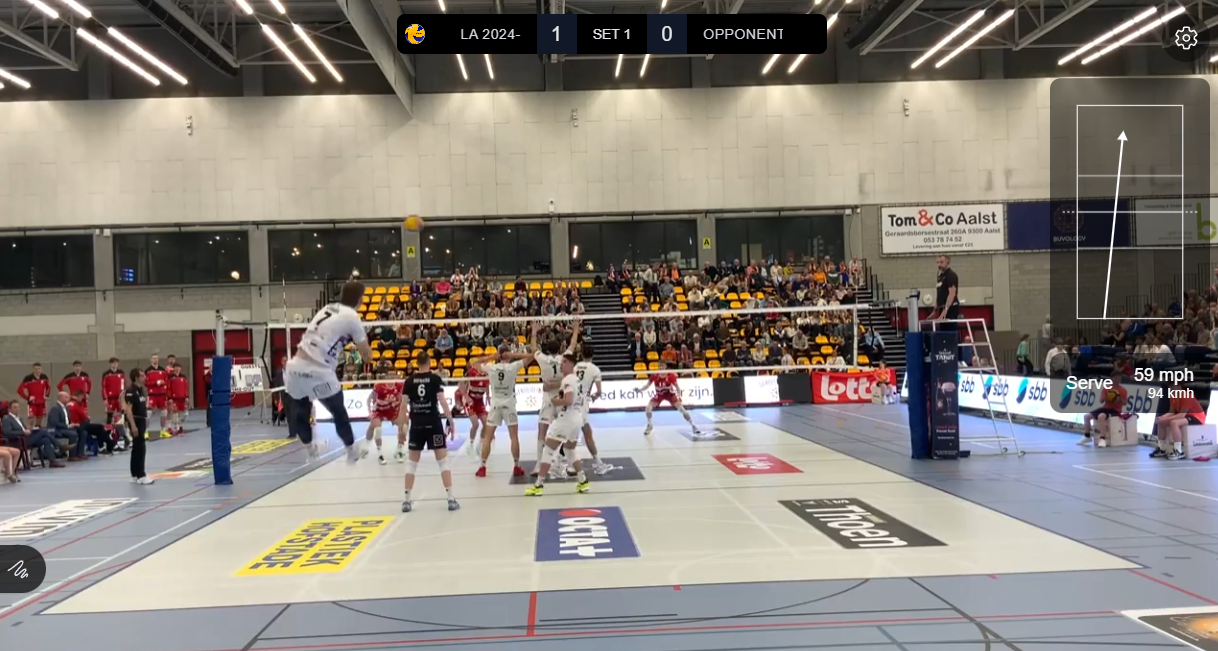
\includegraphics[width=\textwidth]{PL1_AM/opslag.png}
  \caption{\label{fig:PL1_Serve}Voorbeeld van opslagmeting van Balltime AI.}
\end{figure}

Ook in de tweede set, zie tabel \ref{tab:PL1ServeAI2}, valt op dat Balltime AI niet alle snelheden heeft opgemeten. In deze set zijn er 23 metingen gedaan van de 46 opslagen, 50\% van de opslagen. Dit is een verbetering ten opzichte van de eerste set, maar er zijn nog steeds veel snelheden die niet zijn gemeten. De snelheden die wel zijn gemeten, zijn ook hier weer verschillend van de manueel gemeten snelheden. Bij stand 10-9 werd manueel 80 km/u gemeten, terwijl Balltime AI 114 km/u registreerde. Een kleinere afwijking was dan wel weer te vinden bij stand 16-13, waar Balltime AI een snelheid van 41 km/u aangaf tegenover 45 km/u bij de manuele meting. Balltime AI gaf op sommige momenten wel veel hogere waardes, zoals 122 km/u bij 13-11, waar manueel slechts 55 km/u werd gemeten. In deze set lijken er ook enkele consistentere snelheden te zijn gemeten, zoals bij 1-0, waar manueel de meting 93 km/u aangaf en Balltime AI 94 km/u aangaf.

\begin{table}[ht!]
  \centering
  \scriptsize
  \begin{tabular}{|c|c|c|c|} \hline
    L.A.-G.M. & L.A. & G.M. & km/u \\ \hline
    0-0 &  & 19 & 116 \\
    1-0 & 7 & & 93 \\
    1-1 &  & 14 & 50 \\
    2-1 & 1 & & 51 \\
    3-1 & 1 & & 53 \\
    3-2 &  & 10 & 95 \\
    4-2 & 13 & & 89 \\
    4-3 &  & 15 & 71 \\
    5-3 & 9 & & 97 \\
    5-4 &  & 2 & 90 \\
    6-4 & 11 & & 82 \\
    6-5 &  & 4 & 61 \\
    7-5 & 14 & & 53 \\
    7-6 &  & 19 & 116 \\
    8-6 & 7 &  & 101 \\
    8-7 &  & 14 & 55 \\
    8-8 &  & 14 & 58 \\
    9-8 & 7 & & 60 \\
    9-9 &  & 10 & 106 \\
    10-9 & 13 & & 80 \\
    11-9 & 13 & & 95 \\
    12-9 & 13 & & 97 \\
    12-10 &  & 15 & 109 \\
    12-11 &  & 15 & 92 \\
    13-11 & 9 &  & 55 \\
    13-12 &  & 2 & 93 \\
    14-12 & 11 &  & 98 \\
    14-13 &  & 4 & 53 \\
    15-13 & 14 &  & 51 \\
    16-13 & 14 &  & 45 \\
    16-14 &  & 19 & 114 \\
    17-14 & 7 &  & 105 \\
    18-14 & 7 &  & 100 \\
    18-15 &  & 14 & 50 \\
    18-16 &  & 14 & 58 \\
    19-16 & 3 &  & 106 \\
    20-16 & 3 &  & 98 \\
    20-17 &  & 10 & 105 \\
    21-17 & 13 &  & 97 \\
    22-17 & 13 &  & 106 \\
    23-17 & 13 &  & 100 \\
    23-18 &  & 15 & 58 \\
    23-19 &  & 15 & 79 \\
    24-19 & 9 &  & 98 \\
    24-20 &  & 2 & 108 \\
    24-21 &  & 2 & 101 \\
    25-21 &  &  &  \\ \hline
  \end{tabular}
  \caption[Manueel gemeten opslagsnelheden tijdens set 2]{\label{tab:PL1ServeMan2}Manueel gemeten opslagsnelheden tijdens set 2.}
\end{table}

\begin{table}[ht!]
  \centering
  \scriptsize
  \begin{tabular}{|c|c|c|c|} \hline
    L.A.-G.M. & L.A. & G.M. & km/u \\ \hline
    0-0 &  & 19 & - \\
    1-0 & 7 & & 94 \\
    1-1 &  & 14 & 56 \\
    2-1 & 1 & & 55 \\
    3-1 & 1 & & 59 \\
    3-2 &  & 10 & - \\
    4-2 & 13 & & - \\
    4-3 &  & 15 & - \\
    5-3 & 9 & & - \\
    5-4 &  & 2 & 95 \\
    6-4 & 11 & & - \\
    6-5 &  & 4 & - \\
    7-5 & 14 & & 71 \\
    7-6 &  & 19 & - \\
    8-6 & 7 &  & 70 \\
    8-7 &  & 14 & 54 \\
    8-8 &  & 14 & 43 \\
    9-8 & 7 & & 73 \\
    9-9 &  & 10 & 92 \\
    10-9 & 13 & & 114 \\
    11-9 & 13 & & 109 \\
    12-9 & 13 & & 98 \\
    12-10 &  & 15 & - \\
    12-11 &  & 15 & 74 \\
    13-11 & 9 &  & 122 \\
    13-12 &  & 2 & - \\
    14-12 & 11 &  & - \\
    14-13 &  & 4 & 52 \\
    15-13 & 14 &  & 113 \\
    16-13 & 14 &  & 41 \\
    16-14 &  & 19 & - \\
    17-14 & 7 &  & - \\
    18-14 & 7 &  & 53 \\
    18-15 &  & 14 & 49 \\
    18-16 &  & 14 & - \\
    19-16 & 3 &  & - \\
    20-16 & 3 &  & - \\
    20-17 &  & 10 & - \\
    21-17 & 13 &  & 118 \\
    22-17 & 13 &  & - \\
    23-17 & 13 &  & - \\
    23-18 &  & 15 & - \\
    23-19 &  & 15 & - \\
    24-19 & 9 &  & 33 \\
    24-20 &  & 2 & - \\
    24-21 &  & 2 & - \\
    25-21 &  &  &  \\ \hline
  \end{tabular}
  \caption[Gemeten opslagsnelheden door Balltime AI tijdens set 2]{\label{tab:PL1ServeAI2}Gemeten opslagsnelheden door Balltime AI tijdens set 2.}
\end{table}

%%=============================================================================
%% Conclusie
%%=============================================================================

\chapter{Conclusie}%
\label{ch:conclusie}

% Trek een duidelijke conclusie, in de vorm van een antwoord op de
% onderzoeksvra(a)g(en). Wat was jouw bijdrage aan het onderzoeksdomein en
% hoe biedt dit meerwaarde aan het vakgebied/doelgroep? 
% Reflecteer kritisch over het resultaat. In Engelse teksten wordt deze sectie
% ``Discussion'' genoemd. Had je deze uitkomst verwacht? Zijn er zaken die nog
% niet duidelijk zijn?
% Heeft het onderzoek geleid tot nieuwe vragen die uitnodigen tot verder 
%onderzoek?

Deze bachelorproef onderzocht welke bestaande AI-oplossing voor het automatiseren van volleybalstatistieken het meest geschikt is voor volleybalclub Lindemans Aalst. De aanleiding hiervoor was het ontbreken van geautomatiseerde dataverzameling binnen de club, wat de nauwkeurigheid, snelheid en bruikbaarheid van statistieken beperkte tijdens zowel trainingen als wedstrijden.

Uit de literatuurstudie bleek duidelijk dat AI en machine learning-technologieën al succesvol worden toegepast in verschillende sportdisciplines en aanzienlijke meerwaarde bieden in termen van prestatieanalyse, trainingsoptimalisatie en blessurepreventie. Er werd ook vastgesteld dat in de Liga A van het Belgische volleybal geen enkele club op dit moment gebruikmaakt van AI voor statistiekenverzameling, wat een strategisch voordeel biedt voor Lindemans Aalst om als pionier op te treden.

De requirementsanalyse, gevoed door interviews met coaches, scouters en stafleden, bracht de functionele en technische noden van de club in kaart. Hieruit bleek onder meer de nood aan real-time feedback, een hoge nauwkeurigheid van dataregistratie, gebruiksvriendelijkheid en integratiemogelijkheden met bestaande systemen zoals DataVolley. Daarnaast werd de wens uitgesproken om repetitieve taken te automatiseren en subjectieve fouten bij manuele invoer te minimaliseren.

De vergelijkende studie van bestaande AI-systemen identificeerde Balltime AI als het meest geschikte systeem voor de clubcontext, op basis van criteria zoals nauwkeurigheid, real-time verwerking, compatibiliteit, outputformaten en kosten. Dit systeem werd vervolgens getest in een proof-of-concept tijdens officiële wedstrijden.

Uit de analyse van de praktijktesten bleek dat Balltime AI in staat was om de meeste statistieken even accuraat en in sommige gevallen zelfs accurater dan de manuele methode te registreren. De verwerking gebeurde bovendien sneller en leverde realtime inzichten op die tijdens de wedstrijd benut konden worden. De feedback van de coaches bevestigde de gebruiksvriendelijkheid van het systeem en onderstreepte de meerwaarde van de automatische dataverwerking voor strategische besluitvorming.

Op basis van de resultaten van het onderzoek kan geconcludeerd worden dat automatisering van statistieken via AI een duidelijke meerwaarde biedt voor Lindemans Aalst. Niet alleen worden statistieken sneller en betrouwbaarder verzameld, maar het stelt de technische staf ook in staat om sneller te anticiperen op spelontwikkelingen. De club kan hiermee een voortrekkersrol opnemen binnen de Belgische volleybalwereld.

Tot slot biedt dit onderzoek ook aanbevelingen voor de verdere implementatie van AI binnen sportcontexten, met aandacht voor trainingsmogelijkheden, technische ondersteuning en integratie met bestaande software-infrastructuren. Verder onderzoek kan zich richten op het uitbreiden van AI-analyse naar individuele spelersontwikkeling en blessurepreventie, alsook de toepassing van AI in andere sportdisciplines.


%---------- Bijlagen -----------------------------------------------------------

\appendix

\chapter{Onderzoeksvoorstel}

Het onderwerp van deze bachelorproef is gebaseerd op een onderzoeksvoorstel dat vooraf werd beoordeeld door de promotor. Dat voorstel is opgenomen in deze bijlage.

\section{Samenvatting}

% Kopieer en plak hier de samenvatting (abstract) van je onderzoeksvoorstel.
Bij volleybalclub Lindemans Aalst houden ze momenteel wedstrijdstatistieken handmatig bij en tijdens trainingen leggen ze zelfs geen statistieken vast. Er wordt onderzoek gedaan naar de mogelijkheden en voordelen van de spelers- en matchstatistieken te automatiseren met als doel een competitief voordeel te ontwikkelen. In een sportomgeving waar datagedreven beslissingen en data-analyse nog altijd belangrijker worden, richt dit onderzoek zich op de vraag: \textit{"Welke bestaande AI-oplossing voor volleybalstatistieken te automatiseren biedt de meeste voordelen voor Lindemans Aalst, zowel tijdens wedstrijden als trainingen?"}.
  
Het doel van deze bachelorproef is om via een vergelijkende studie de meest geschikte AI-technologie te selecteren en te implementeren. Hierbij wordt rekening gehouden met aspecten zoals nauwkeurigheid, gebruiksgemak, kosten en toepasbaarheid binnen de context van de club. De methodologie omvat een literatuurstudie naar bestaande AI-oplossingen voor sportanalyse en een praktijkonderzoek waarin de geselecteerde technologie in de dagelijkse werking van Lindemans Aalst wordt getest.

Verwacht wordt dat invoeren van AI de kwaliteit en snelheid van data-analyse zal verhogen, waardoor coaches en spelers ondersteund worden met betere inzichten voor strategische beslissingen en spelersontwikkeling. Dit kan uiteindelijk leiden tot verbeterde prestaties op het veld. Naast voordelen voor Lindemans Aalst kunnen de bevindingen van dit onderzoek ook waardevol zijn voor andere sportclubs die overwegen AI-technologie te integreren voor een datagedreven benadering van trainingen en wedstrijden. 

% Verwijzing naar het bestand met de inhoud van het onderzoeksvoorstel
%---------- Inleiding ---------------------------------------------------------

\section{Inleiding}%
\label{sec:inleiding}

Match- en spelerstatistieken zijn van essentieel belang in de sportwereld. Waarom zijn statistieken belangrijk in de sportwereld en specifiek in volleybal? Bij Lindemans Aalst is het verzamelen van deze gegevens echter nog zeer tijdrovend. Tijdens wedstrijden worden statistieken handmatig bijgehouden, terwijl er tijdens trainingen zelfs geen gegevens worden verzameld. Dit handmatige proces is niet alleen inefficiënt, maar kan ook leiden tot inconsistenties in de data.

Automatisering van statistieken biedt potentieel voor een systeem dat in staat is realtime statistieken vast te leggen, zowel tijdens wedstrijden als trainingen, wat leidt tot een efficiënte en betrouwbare dataverzameling. Welke technologieën worden momenteel gebruikt voor het automatiseren van sportstatistieken? Hoe presteren bestaande AI-systemen voor het verzamelen en analyseren van volleybalstatistieken?

Automatisering zou ervoor zorgen dat er minder fouten aanwezig zijn en dat de statistieken sneller beschikbaar zijn. Dit zou er dan weer voor zorgen dat de coaches sneller en beter beslissingen kunnen maken. Daarom dus: \textit{"Welke bestaande AI-oplossing voor het automatiseren van volleybalstatistieken biedt de meeste voordelen voor Lindemans Aalst, zowel tijdens wedstrijden als trainingen?"}
%---------- Stand van zaken ---------------------------------------------------

\section{Literatuurstudie}%
\label{sec:literatuurstudie}
% Voor literatuurverwijzingen zijn er twee belangrijke commando's:
% \autocite{KEY} => (Auteur, jaartal) Gebruik dit als de naam van de auteur
%   geen onderdeel is van de zin.
% \textcite{KEY} => Auteur (jaartal)  Gebruik dit als de auteursnaam wel een
%   functie heeft in de zin (bv. ``Uit onderzoek door Doll & Hill (1954) bleek
%   ...'')
% Inleiding, wat is het belang van statistieken in de sportwereld
Geautomatiseerde dataverzameling en -analyse spelen een steeds grotere rol in de professionele sportwereld, waar nauwkeurige statistieken noodzakelijk zijn voor prestatieverbetering en strategische besluitvorming. In de sport, in het bijzonder in volleybal, zorgt automatisering van statistiekenverzameling ervoor dat spelers en coaches beter inzicht krijgen in prestaties, waardoor training en wedstrijdvoorbereiding doelgerichter kunnen worden aangepakt.
\subsection{Belang van statistieken in de sportwereld}
Vooral technologieën zoals AI, computer vision en machine learning bieden nieuwe mogelijkheden om spelmomenten en spelersbewegingen nauwkeurig vast te leggen en te analyseren. De spelers- en matchstatistieken \autocite{Wahyuti2023} zijn van uiterst belang. Ze bieden niet alleen inzichten in de puntenregistratie van het team, maar ook in de tactische en technische aspecten van het spel. Volgens de studie is het belangrijk om een uitgebreid digitaal puntenregistratie bij te houden. Dit om fouten en verlies van gegevens te minimaliseren. Dit komt echter vaak voor bij handmatige invoer. Uit onderzoek \autocite{Harabagiu2023} blijkt dat door het gebruik van door gebruik van de statistische software Data Volley de efficiënte van een team met 6\% stijgt. De software identificeert de tekortkomingen en hierdoor kunnen individuele trainingsprogramma's opgesteld worden voor elke speler. Volgens \textcite{Ruiye2024} zijn de nauwkeurigheid en efficiëntie van de videoanalyse zeer belangrijk. Een innovatief videoanalysemodel gebaseerd op Bi-directional Long Short-Term Memory (BiLSTM) en aandachtsmechanismen behaalt een herkenningsnauwkeurigheid van meer dan 90\%.

Natuurlijk zijn er andere invloeden op de statistieken dan alleen de spelersprestaties \autocite{LopezSerrano2022}. Zo spelen volgens verschillende coaches het niveau van de tegenstander, het moment in een set, het scoreverschil, resultaat van de vorige set en het de competitieve druk een zeer grote in de analyse. Trainers pleiten ervoor dat er een geïntegreerde benadering is voor deze variabelen. Hierdoor wordt rekening gehouden met de specifieke omstandigheden van elke wedstrijd. Deze gegevens mogen niet geïsoleerd worden bekeken, maar juist in samenhang geanalyseerd. Bij verder onderzoek is het van essentieel belang dat coaches worden betrokken bij de ontwikkeling hiervan.
% Bestaande AI-oplossingen voor sportstatistieken

% Gebruik van sensors en camera's voor dataverzameling
\subsection{Gebruik van sensors en camera's voor dataverzameling}
Uit onderzoek van Xu \textcite{Sun2021} blijkt dat door de vooruitgang in elektronische en sensortechnologieën is het mogelijk geworden om menselijke bewegingen en spelmomenten nauwkeurig vast te leggen. In de sportwereld zijn sensoren en camera's steeds vaker te vinden op en naast het veld. Deze technologieën maken het mogelijk om realtime data te verzamelen over spelersposities, balbewegingen en spelsituaties door middel van sensoren aan de gewrichten van spelers te bevestigen. Door deze data te analyseren met behulp van AI-algoritmen kunnen coaches en analisten waardevolle inzichten verkrijgen in de prestaties en strategieën.

\textcite{Liang2023} concludeerden dat traditionele videoanalysemethode vaak te beperkt zijn voor de variabele omstandigheden zoals verlichting en achtergrond tijdens het spel. Skeletdata biedt hier een oplossing voor door de bewegingen van spelers te vereenvoudigen tot een netwerk van verbonden gewrichten. De complexiteit van de visuele gegevens vermindert hierdoor. De methode zou nog een extra assistentie kunnen bieden aan de coaches en spelers.
%---------- Methodologie ------------------------------------------------------
\section{Methodologie}%
\label{sec:methodologie}

Elke week die beschreven wordt bestaat uit 1 volledige dag werk aan de bachelorproef.
\subsection{Fase 1: Literatuurstudie}
De literatuurstudie is bedoeld om inzicht te krijgen in de huidige stand van zaken met betrekking tot AI-systemen die geschikt zijn voor het verzamelen en analyseren van sportstatistieken. Waarom zijn statistieken belangrijk in de sportwereld en specifiek in volleybal? Deze vraag wordt beantwoord door het analyseren van academische publicaties en praktijkvoorbeelden. Daarnaast worden whitepapers en technische documentatie van bekende AI-tools, zoals Hudl, DataVolley, Second Spectrum en Balltime AI, bestudeerd.

De focus ligt hierbij op het beoordelen van nauwkeurigheid, snelheid, schaalbaarheid en kosten van deze systemen, omdat deze factoren belangrijk zijn voor de toepassing binnen Lindemans Aalst. Welke technologieën worden momenteel gebruikt voor het automatiseren van sportstatistieken? Dit wordt onderzocht door een overzicht te creëren van bestaande systemen en technologieën.

Aan het einde van deze fase wordt een overzichtsrapport opgesteld met de bevindingen, waarin ook een vergelijkingstabel wordt opgenomen die de sterke en zwakke punten van elk systeem schetst. Dit rapport vormt de basis voor de selectie van systemen die in latere fases verder onderzocht zullen worden. Deze fase duurt 2 weken.
\subsection{Fase 2: Interviews en requirementsanalyse}
In de tweede fase, die 1 week duurt, worden gestructureerde interviews afgenomen met de coaches, data-analisten en technische staf van Lindemans Aalst. Het doel van deze interviews is om een duidelijk beeld te krijgen van de functionele en technische eisen die de club stelt aan een geautomatiseerd statistieken systeem. \textit{"Hoe presteren bestaande AI-systemen voor het verzamelen en analyseren van volleybalstatistieken?"} en \textit{"Welke technologieën worden momenteel gebruikt voor het automatiseren van sportstatistieken?"}. Deze vragen worden besproken met stakeholders, waarbij hun ervaringen en verwachtingen worden genoteerd.

De requirementsanalyse richt zich op de statistieken die essentieel zijn voor de club en op specifieke analyses die coaches tijdens wedstrijden en trainingen nodig hebben. De inzichten uit deze gesprekken worden verwerkt in een requirementsdocument, dat de functionele en technische vereisten vastlegt. Dit document vormt een referentiepunt voor de vergelijkende analyse van de AI-systemen in de volgende fase.
\subsection{Fase 3: Vergelijkende studie van AI-systemen}
In deze 3 weken durende fase worden de geselecteerde AI-systemen geëvalueerd op basis van nauwkeurigheid, snelheid en gebruiksgemak, om objectief te bepalen welke oplossing het best aansluit bij de eisen van Lindemans Aalst. Hiervoor wordt gebruikgemaakt van eerder verzamelde datasets van match- en trainingsgegevens. \textit{"Hoe presteren bestaande AI-systemen voor het verzamelen en analyseren van volleybalstatistieken?"} wordt verder onderzocht door de prestaties van de systemen in de praktijk te testen en te vergelijken met handmatig geregistreerde data.

De systemen worden getest op hun vermogen om deze data nauwkeurig en snel te verwerken. Het rapport bevat ook een concrete aanbeveling van het systeem dat het meest geschikt lijkt voor implementatie, op basis van de vergelijking.
\subsection{Fase 4: Proof of concept en praktijktest}
Na de vergelijkende studie wordt het aanbevolen systeem geïmplementeerd als proof of concept (PoC) bij Lindemans Aalst, op voorwaarde dat het seizoen nog bezig is. Deze praktijktest van 3 weken heeft als doel te valideren of het systeem daadwerkelijk voldoet aan de functionele en technische eisen van de club. Gedurende deze periode verzamelt het systeem automatisch gegevens tijdens trainingen en wedstrijden, zodat coaches en analisten het gebruiksgemak en de nauwkeurigheid van de automatisering kunnen evalueren.

De prestaties van het PoC-systeem worden vergeleken met handmatig geregistreerde gegevens en de feedback van de coaches over de gebruiksvriendelijkheid wordt verzameld. Aan het einde van deze fase wordt een validatierapport opgesteld, waarin de kwantitatieve resultaten van het geautomatiseerde systeem zijn opgenomen, evenals eventuele aanbevelingen voor optimalisatie.
\subsection{Fase 5: Analyse en eindrapport}
In de laatste fase, die nog 2 weken zal duren, worden de resultaten van het onderzoek geanalyseerd en samengebracht in een eindrapport. Dit rapport bevat een grondige analyse van de prestaties van het PoC-systeem en conclusies over de mate waarin het systeem de doelstellingen van Lindemans Aalst ondersteunt. \textit{"Waarom zijn statistieken belangrijk in de sportwereld en specifiek in volleybal?"} wordt in deze fase opnieuw geëvalueerd op basis van de praktische resultaten.

De data uit de eerdere fases worden statistisch geanalyseerd om objectieve conclusies te trekken over de invloed van automatisering op de nauwkeurigheid en snelheid van statistiekenregistratie. Het rapport bevat zowel aanbevelingen voor de club over de definitieve implementatie van het AI-systeem als suggesties voor toekomstige optimalisaties.

\begin{figure}[ht]
  \centering
  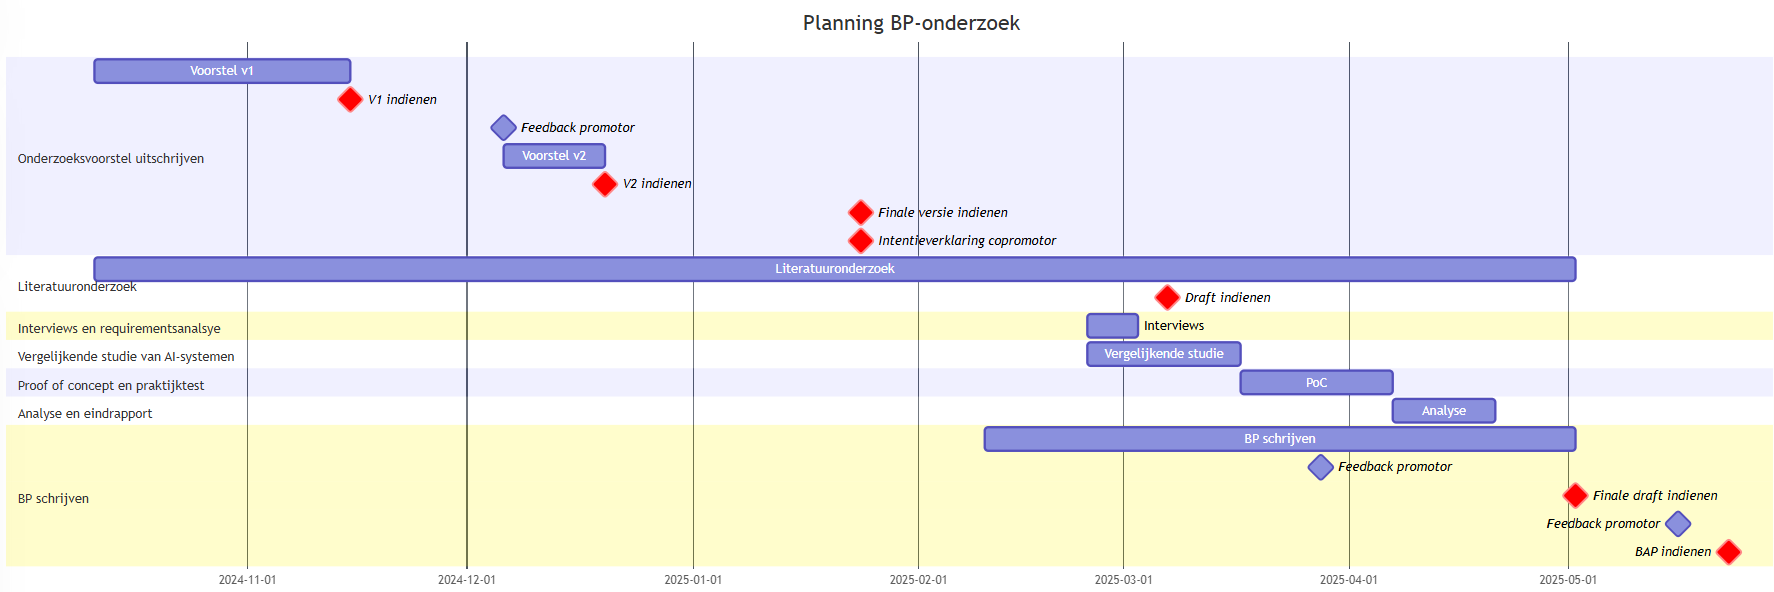
\includegraphics[width=0.5\textwidth]{img/gantt.png}
  \caption{\label{fig:gantt}Gantt planning bachelorproef}
\end{figure}

\begin{figure}[ht]
  \centering
  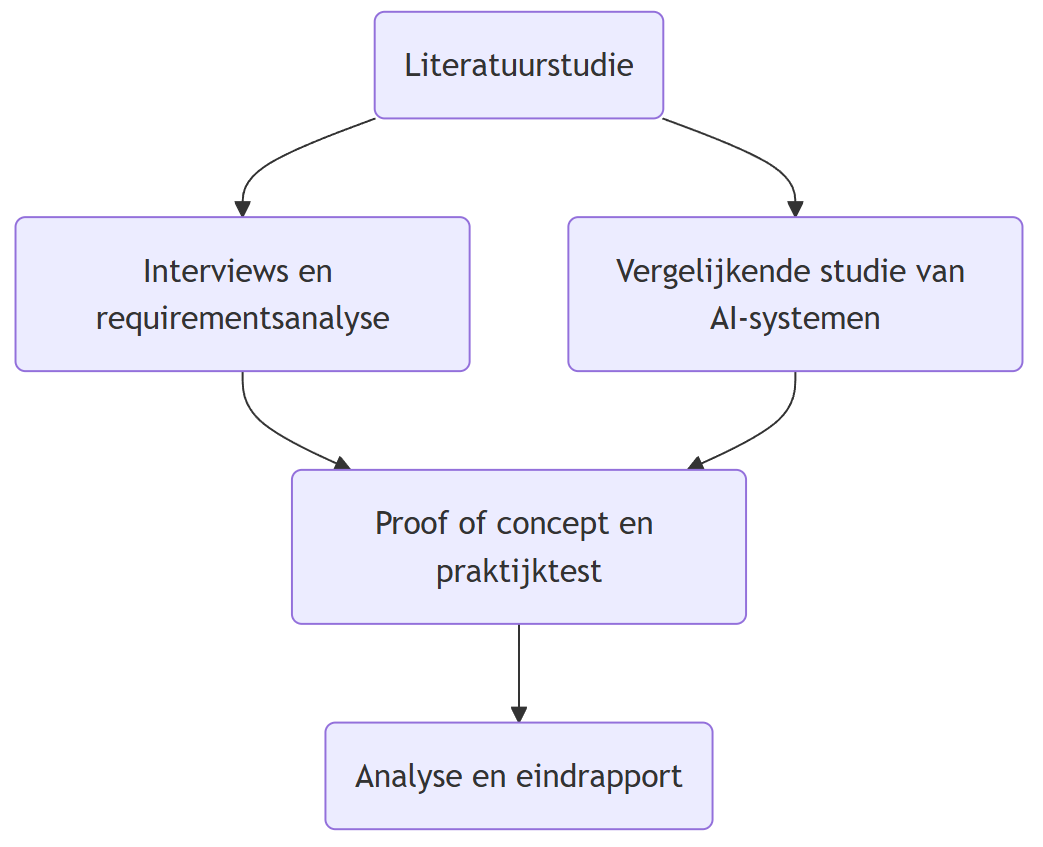
\includegraphics[width=0.3\textwidth]{img/flowchart.png}
  \caption{\label{fig:flowchart}Flowchart bachelorproef}
\end{figure}

%---------- Verwachte resultaten ----------------------------------------------
\section{Verwacht resultaat, conclusie}%
\label{sec:verwachte_resultaten}
Dit onderzoek richt zich op het automatiseren van spelers- en matchstatistieken bij volleybalclub Lindemans Aalst en beoogt een positieve invloed op de nauwkeurigheid en snelheid van dataverzameling, waarmee de club strategisch betere keuzes kan maken. Momenteel worden statistieken tijdens wedstrijden handmatig bijgehouden, terwijl er tijdens trainingen zelfs geen gegevens worden verzameld. Dit handmatige proces is tijdrovend en kan leiden tot inconsistenties in de data. Automatisering biedt potentieel voor een systeem dat in staat is realtime statistieken vast te leggen, zowel tijdens wedstrijden als trainingen, wat resulteert in een meer efficiënte en betrouwbare dataverzameling.

Allereerst wordt een verbetering verwacht in de nauwkeurigheid van gegevensverzameling. Het geautomatiseerde systeem zal naar verwachting 15-25\% nauwkeuriger zijn dan de handmatige methode door het verminderen van menselijke fouten.

Daarnaast wordt een aanzienlijke tijdsbesparing verwacht in de snelheid van data-analyse. Door een AI-gestuurd systeem toe te passen, kan de tijd voor gegevensverwerking en analyse met 30-50\% worden verminderd, wat vooral waardevol is tijdens het dynamische wedstrijdmoment. Het systeem maakt gegevens direct beschikbaar, zodat coaches en spelers tijdens wedstrijden hun beslissingen onmiddellijk kunnen aanpassen aan de realtime prestaties van het team.

Bovendien wordt verwacht dat het systeem de tactische beslissingen en trainingsinzichten van de coaches aanzienlijk zal verbeteren. Met de beschikbaarheid van gedetailleerde statistieken tijdens en na wedstrijden en trainingen zullen coaches in staat zijn om beslissingen te nemen op basis van een hogere kwaliteit en kwantiteit aan data.

De meerwaarde voor Lindemans Aalst ligt in drie hoofdgebieden: betere en snellere besluitvorming, efficiëntieverbetering en langetermijninzicht. Door realtime inzicht te krijgen in prestaties, zowel tijdens wedstrijden als trainingen, kunnen coaches gefundeerde keuzes maken, tijd besparen en diepgaandere analyses uitvoeren. Het systeem voegt waarde toe door historische gegevens op te slaan, waardoor coaches trends en de ontwikkeling van spelers effectief kunnen volgen. De resultaten van dit onderzoek bieden niet alleen een waardevolle tool voor Lindemans Aalst, maar verschaffen ook inzichten die andere sportorganisaties kunnen inspireren om AI-technologieën voor datagedreven analyse en besluitvorming te implementeren.

%%---------- Andere bijlagen --------------------------------------------------
% Voeg hier eventuele andere bijlagen toe. Bv. als je deze BP voor de
% tweede keer indient, een overzicht van de verbeteringen t.o.v. het origineel.
%\input{...}
\chapter{Afkortingen}
\label{ch:afkortingen}
\begin{description}
    \item[Tot] Totaal
    \item[SA] Serve Aces
    \item[SE] Serve Errors / Set Errors
    \item[TA] Total Attempts
    \item[Pct] Percentage that are not errors
    \item[Eff] Efficiency
    \item[Rtg] 
    \item[Pass\%] Avarage pass rating
    \item[Perfect PP] Percentage of perfect passes
    \item[Good PP] Percentage of good passes
    \item[Ast] Assists
    \item[A/S] Assists per set
    \item[DS] Number of successful digs
    \item[DE] Number of digs that resulted in a point for the other team
    \item[K] Kills
    \item[E] Errors
    \item[Atk\%] Attack efficiency
    \item[Kill\%] Kill percentage
    \item[Error\%] Error percentage
    \item[BS] Number of blocks resulting in a point when the player is the only blocker
    \item[BA] Number of blocks resulting in a point when the player is one of multiple blockers
    \item[BE] Number of blocks where the player was called for a net violation
    \item[B/S] Blocks per set         
\end{description}

\chapter{Statistieken van de wedstrijden}
De statistieken in deze bijlage zijn manueel verzameld en ingevoerd door de scouter van Lindemans Aalst tijdens 2 wedstrijden. Ze vormen een belangrijk basis voor de vergelijkende studie van de statistieken in deze bachelorproef.

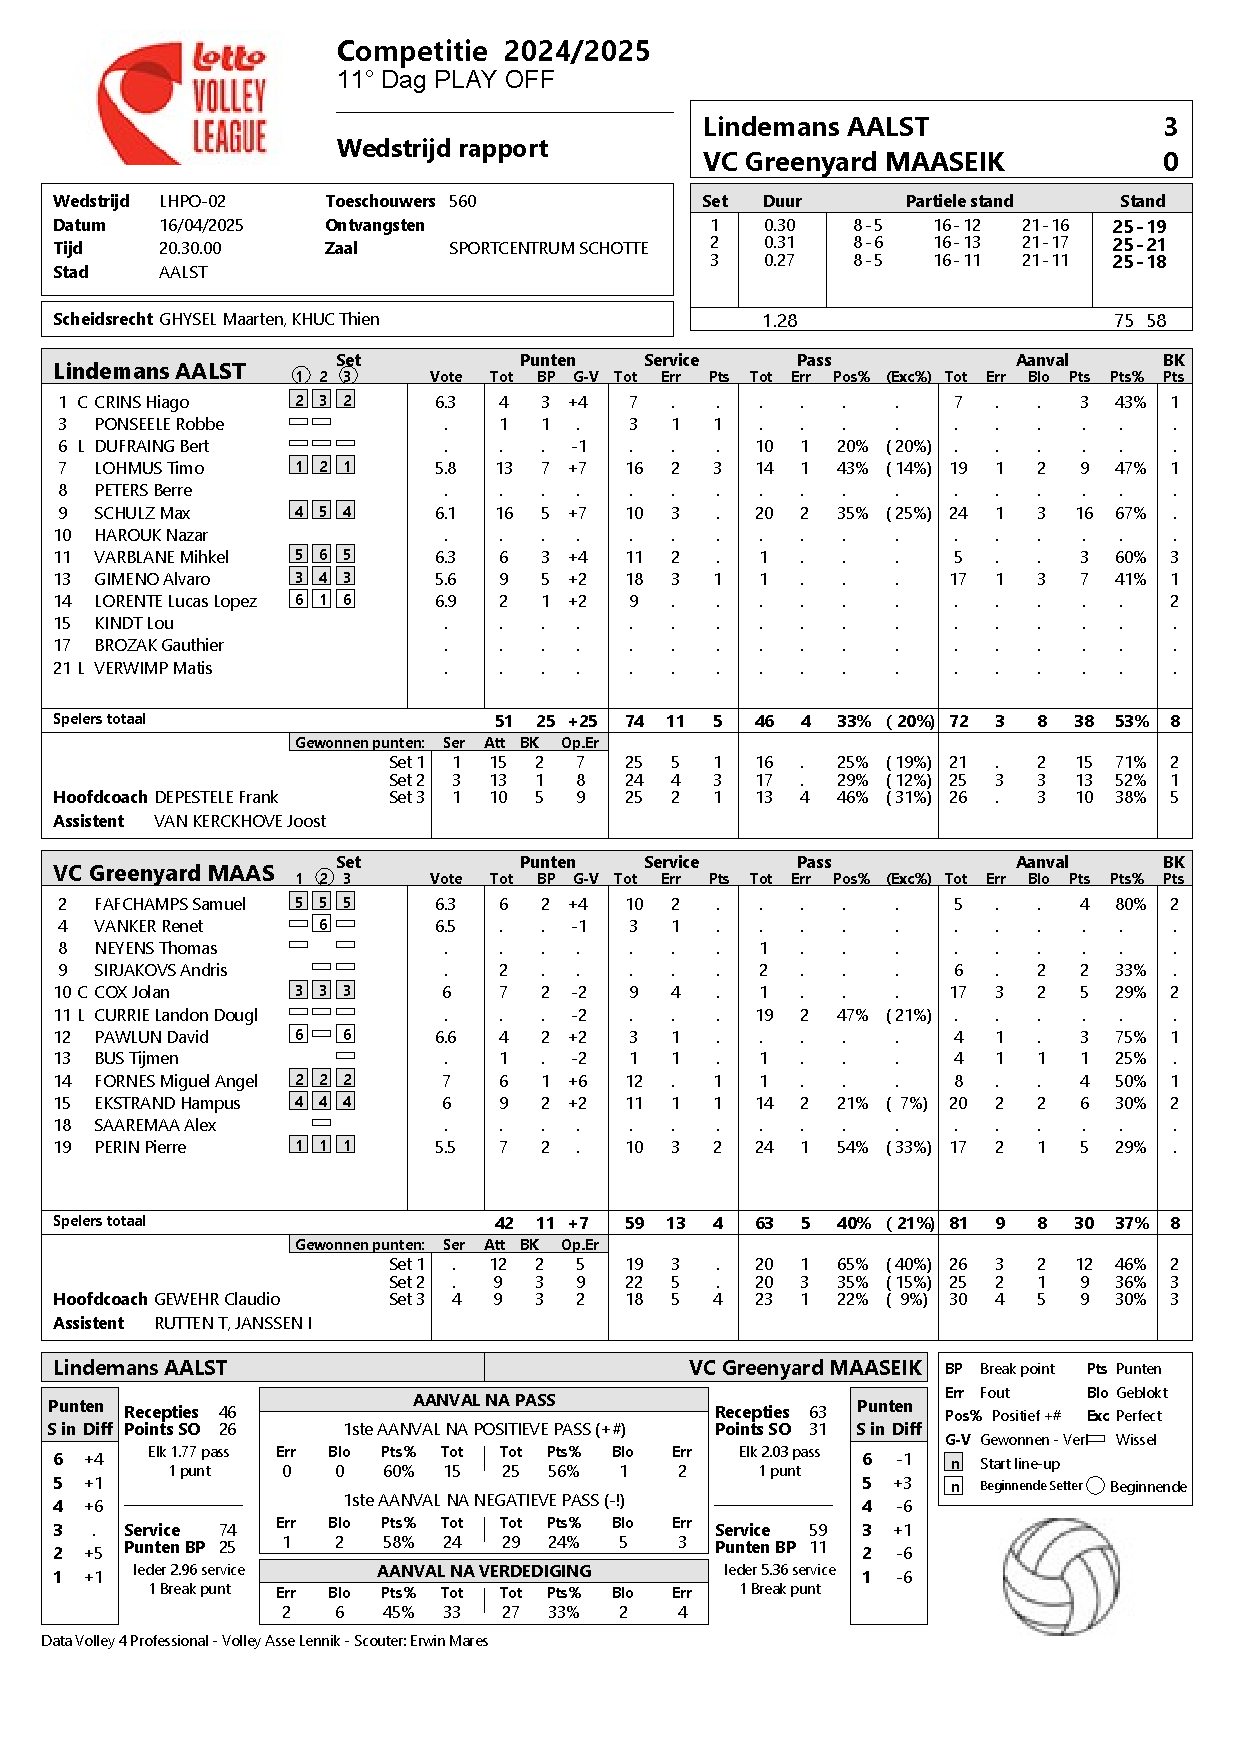
\includepdf[pages=-]{../inserts/20250416_LHPO02_aalst_maaseik.pdf}
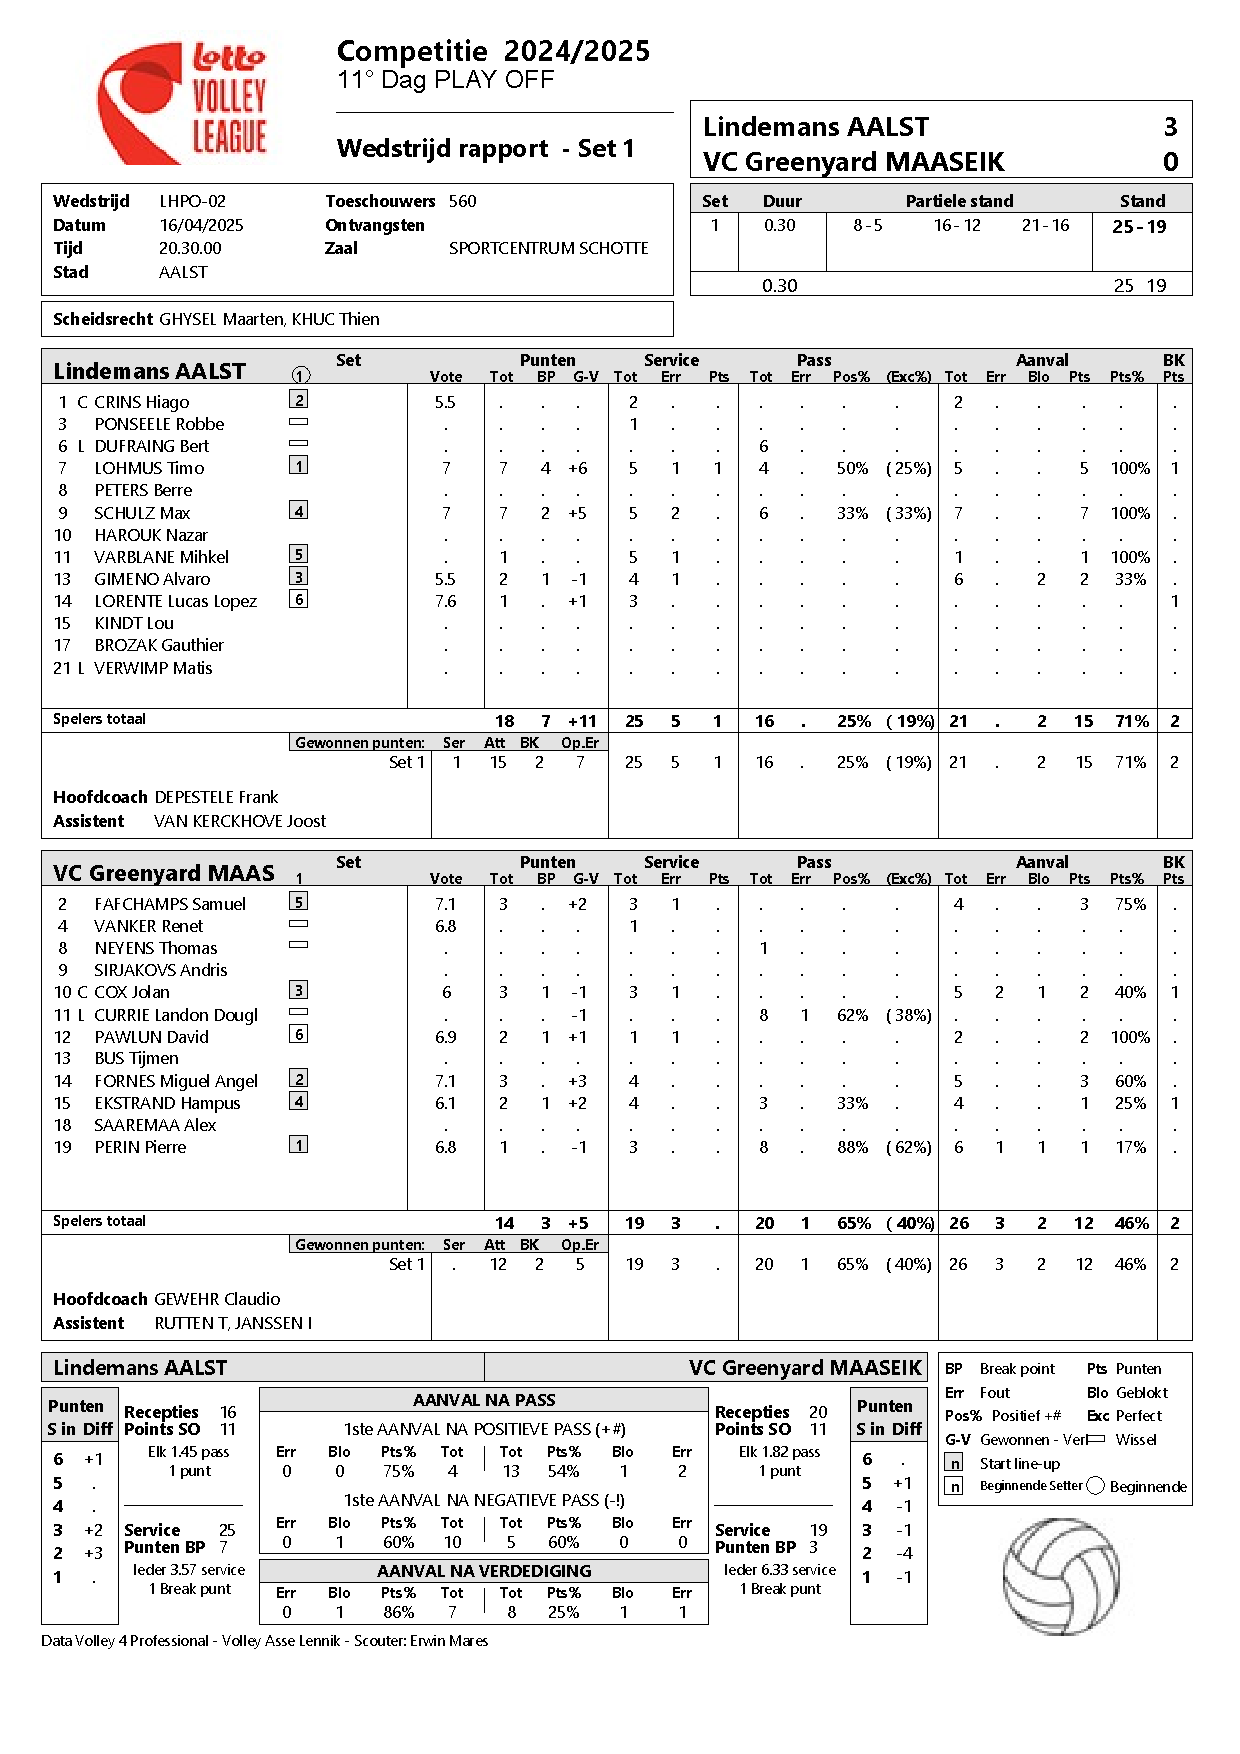
\includepdf[pages=-]{../inserts/20250416_LHPO02_aalst_maaseik_set1.pdf}
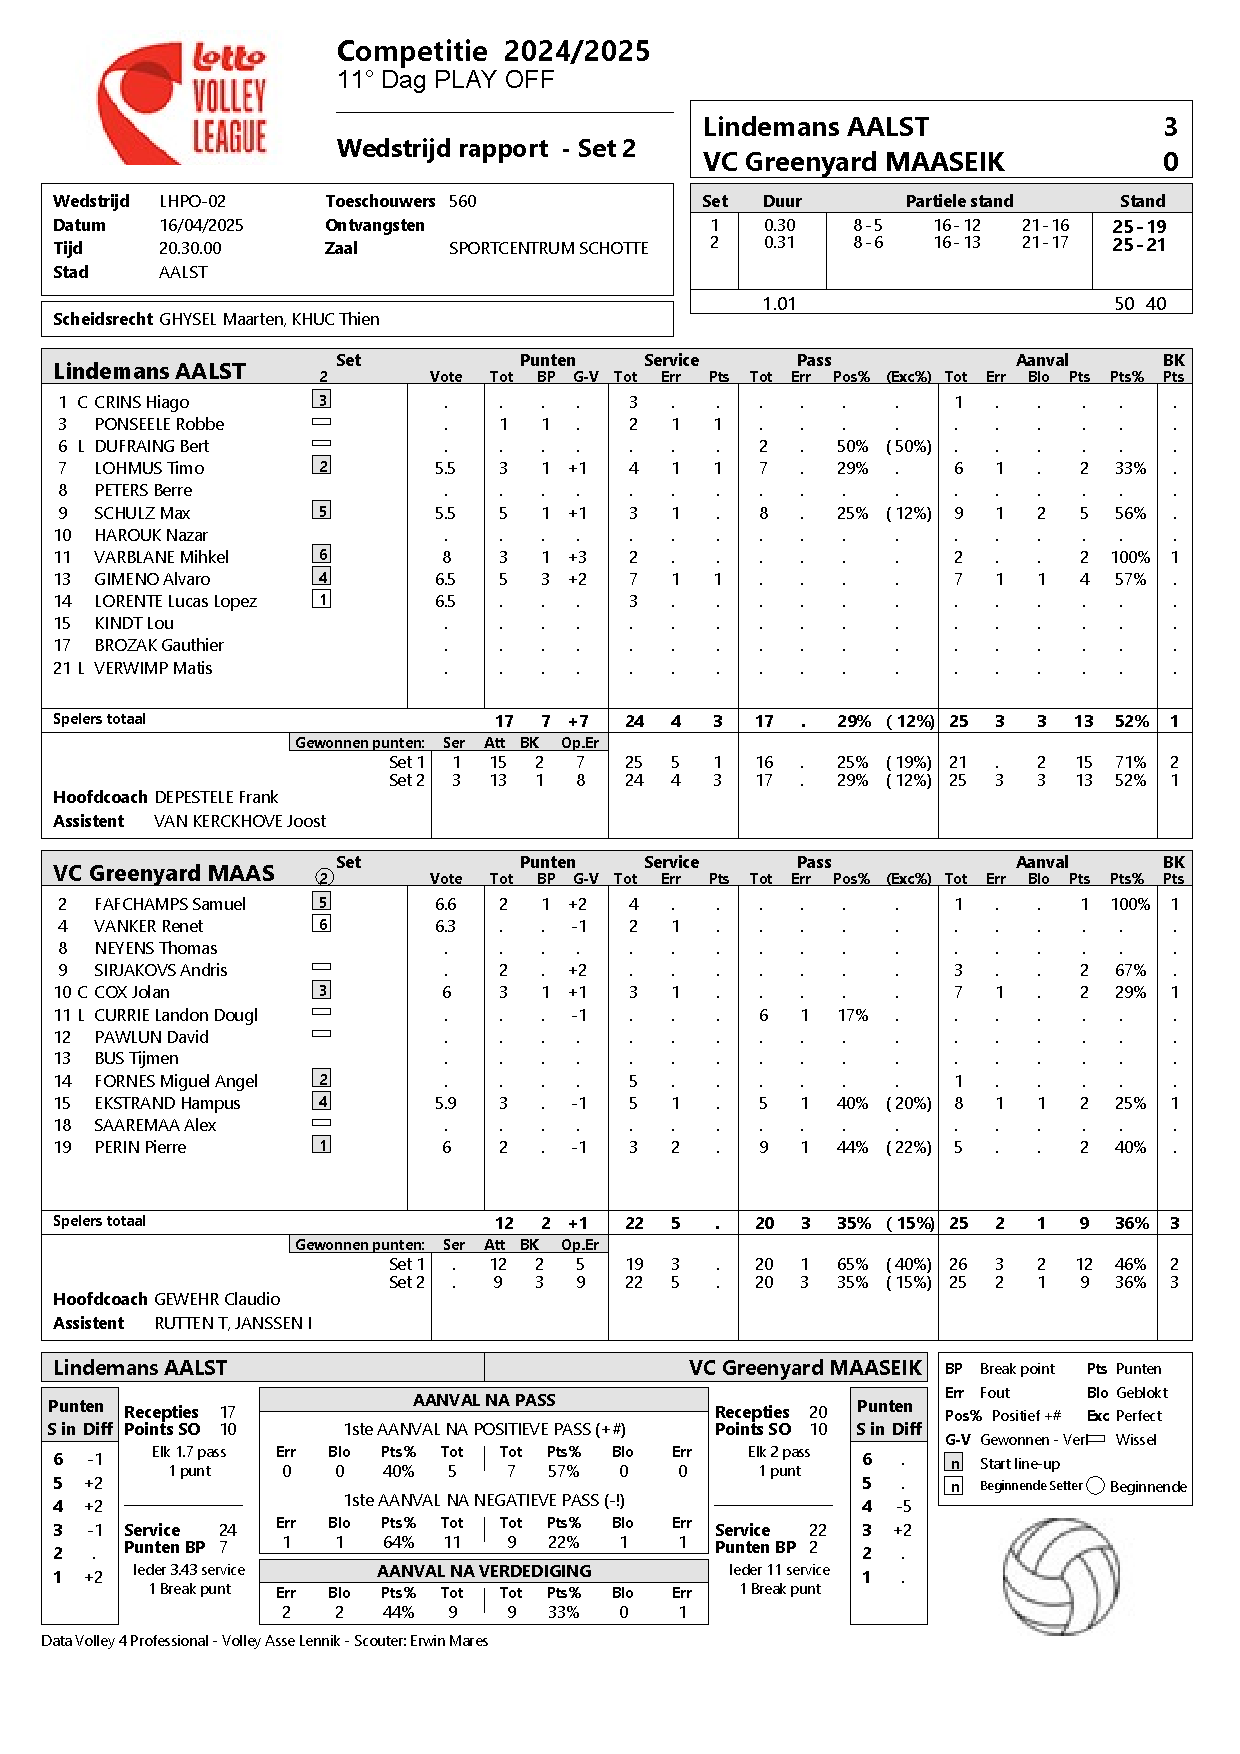
\includepdf[pages=-]{../inserts/20250416_LHPO02_aalst_maaseik_set2.pdf}
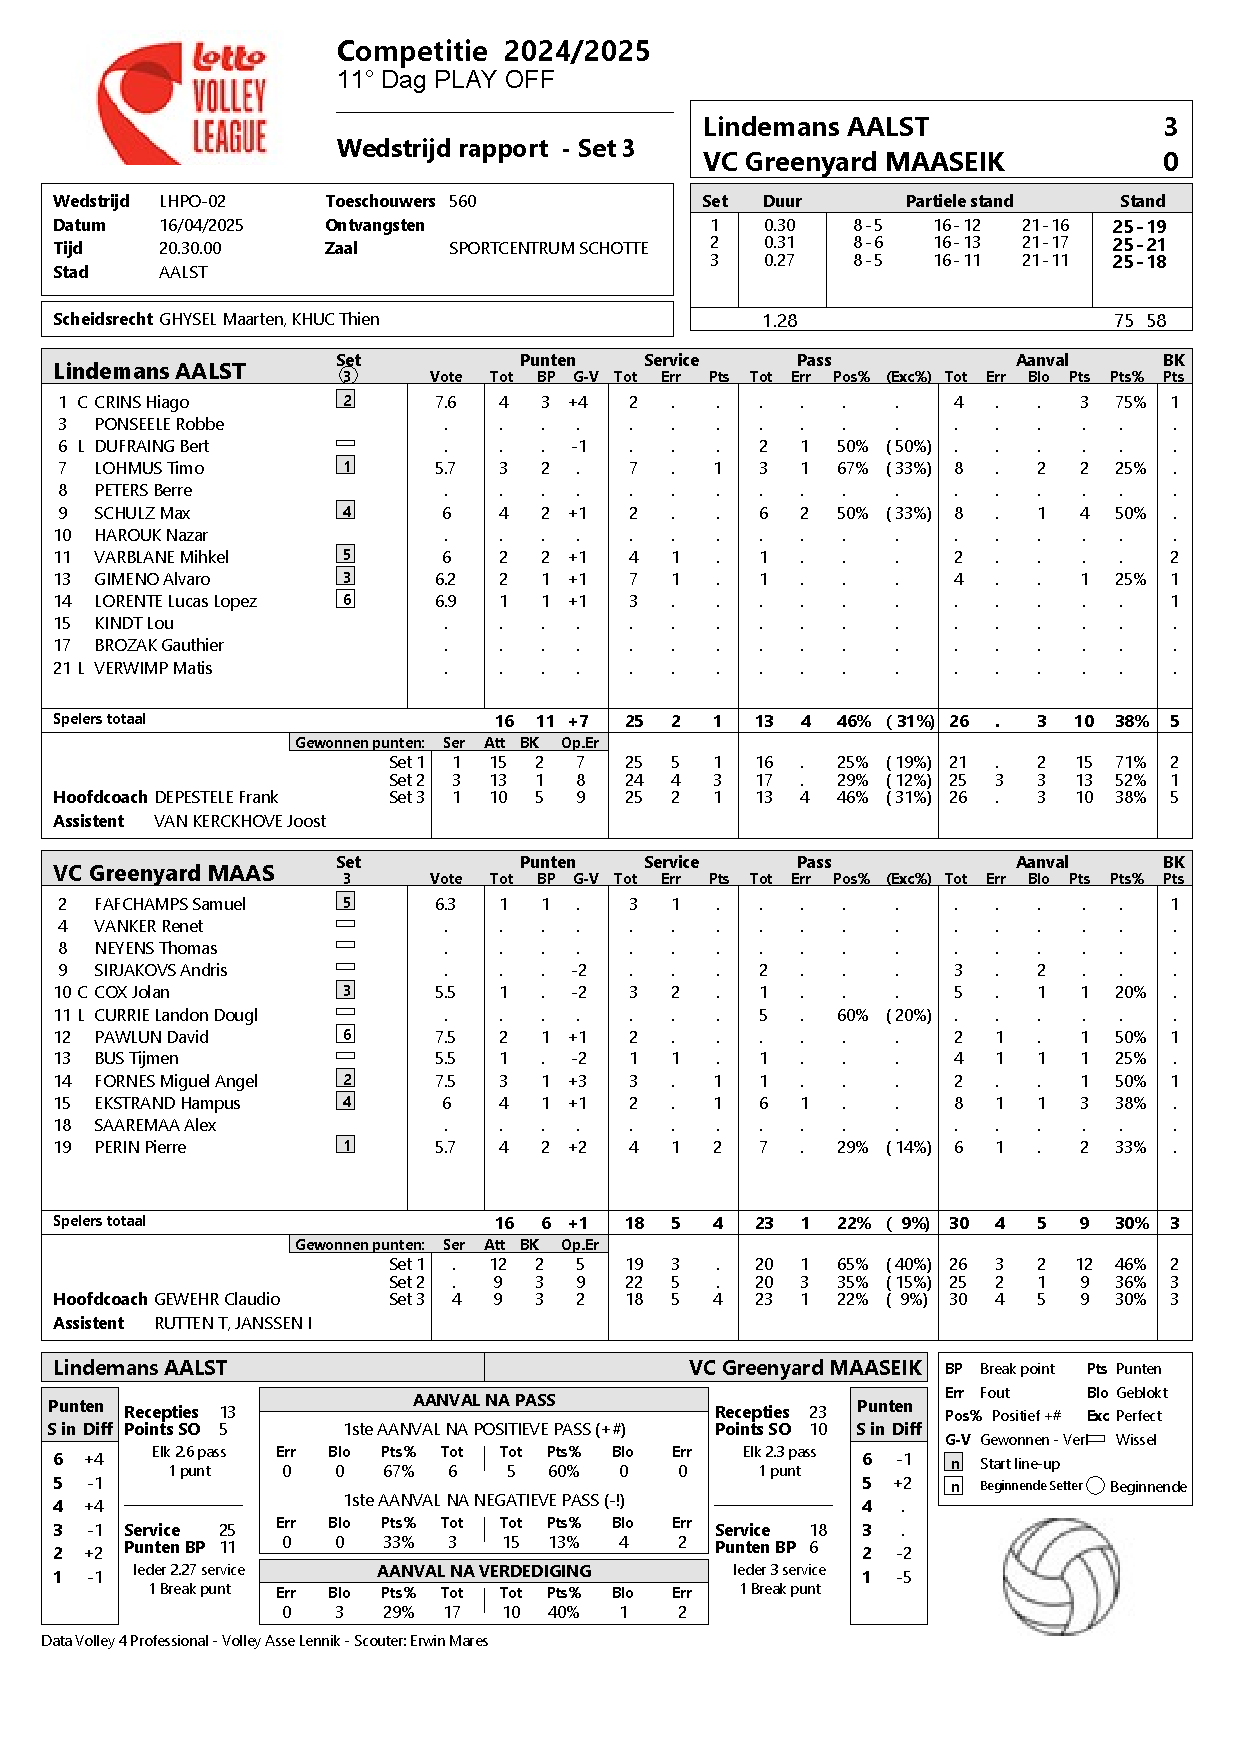
\includepdf[pages=-]{../inserts/20250416_LHPO02_aalst_maaseik_set3.pdf}
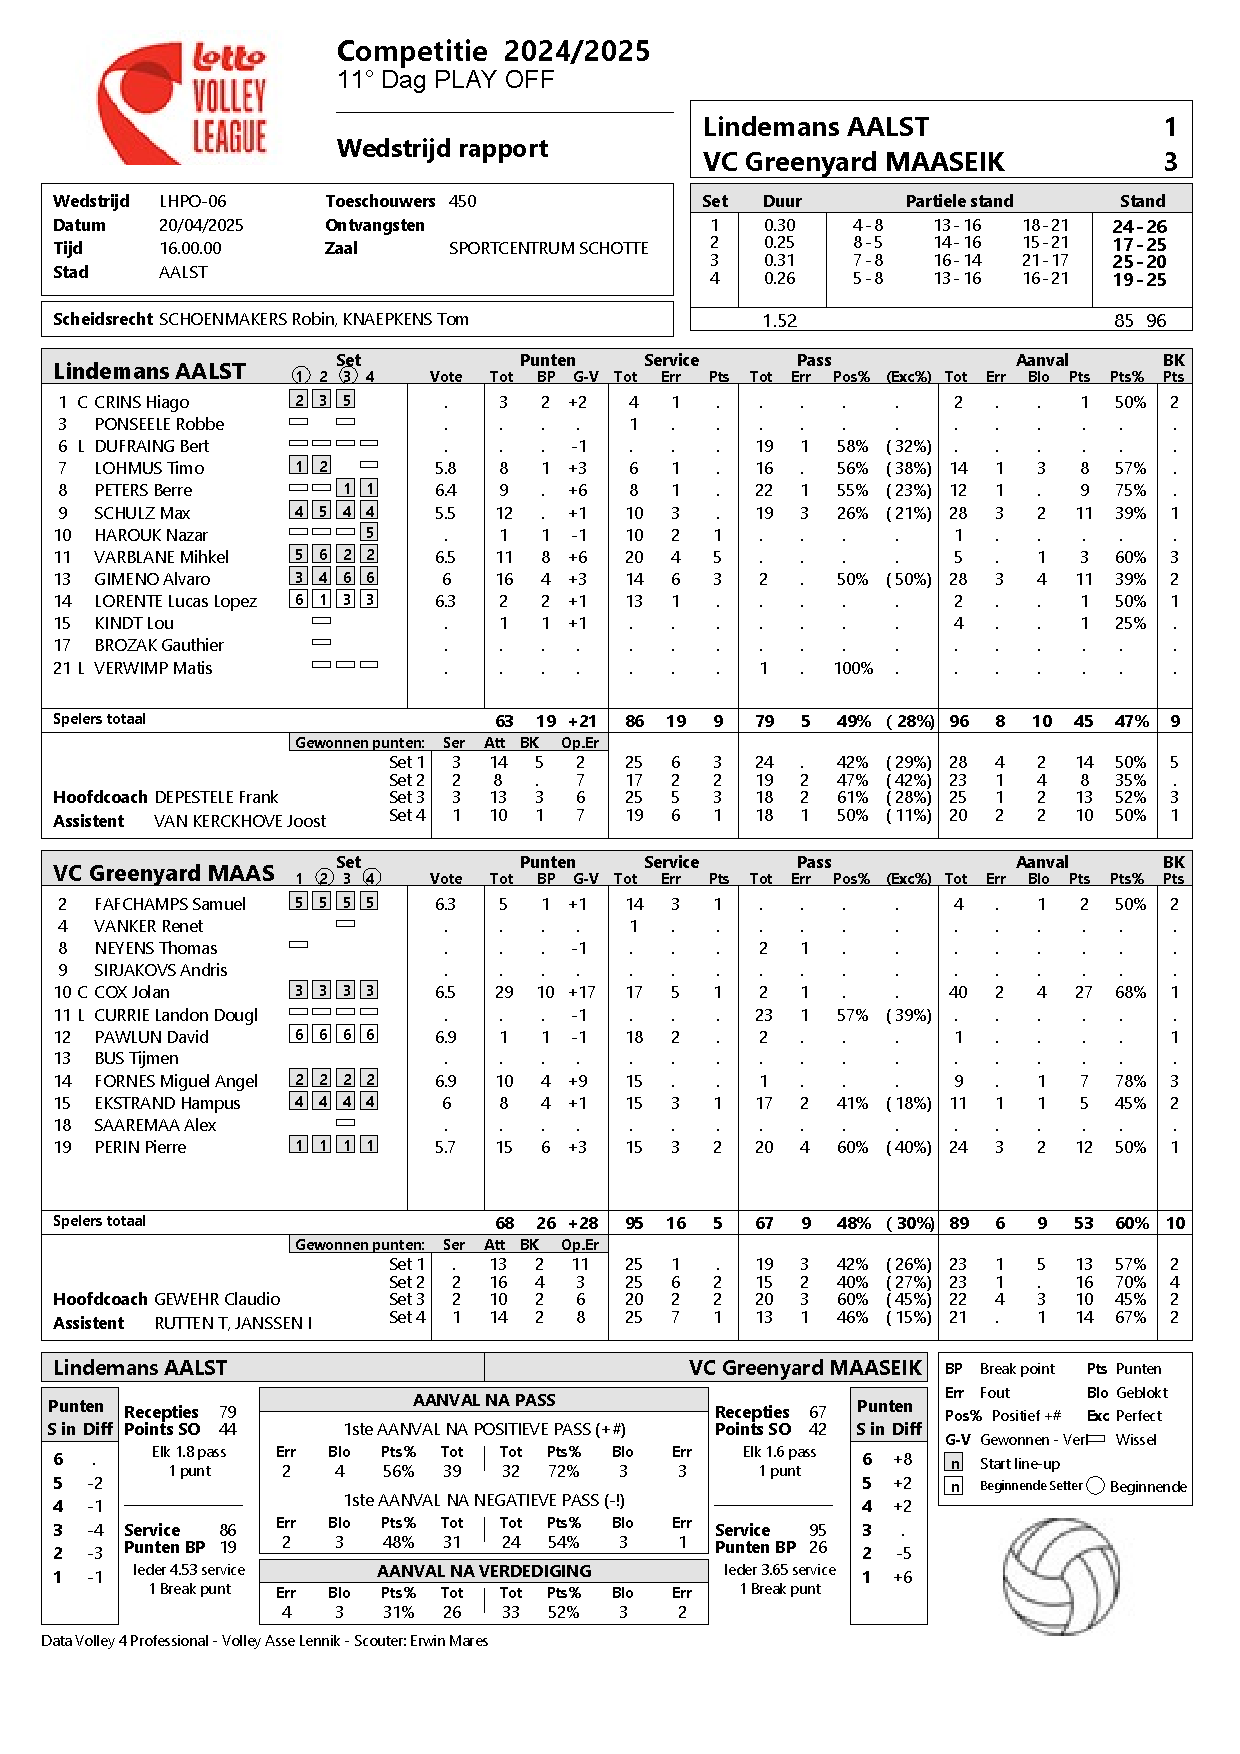
\includepdf[pages=-]{../inserts/20250420_LHPO06_aalst_maaseik.pdf}
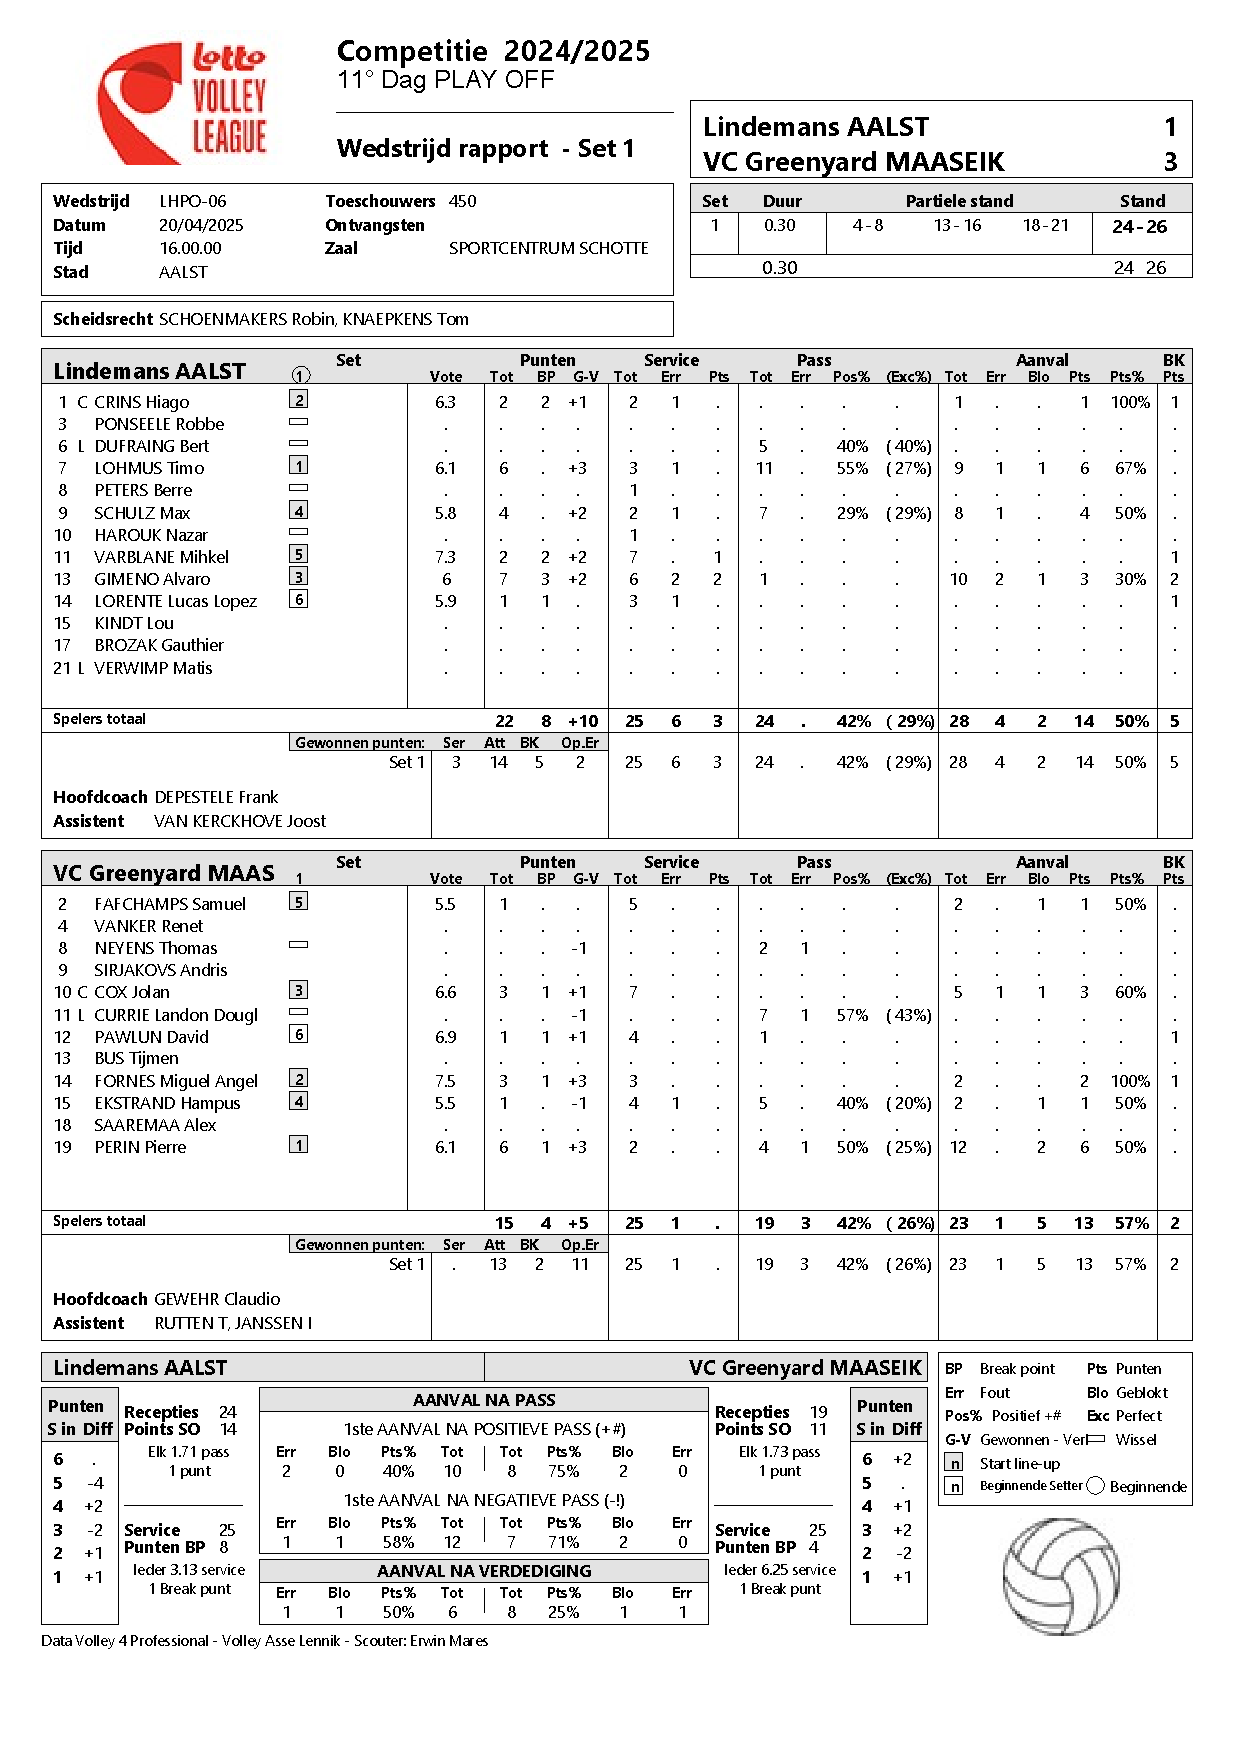
\includepdf[pages=-]{../inserts/20250420_LHPO06_aalst_maaseik_set1.pdf}
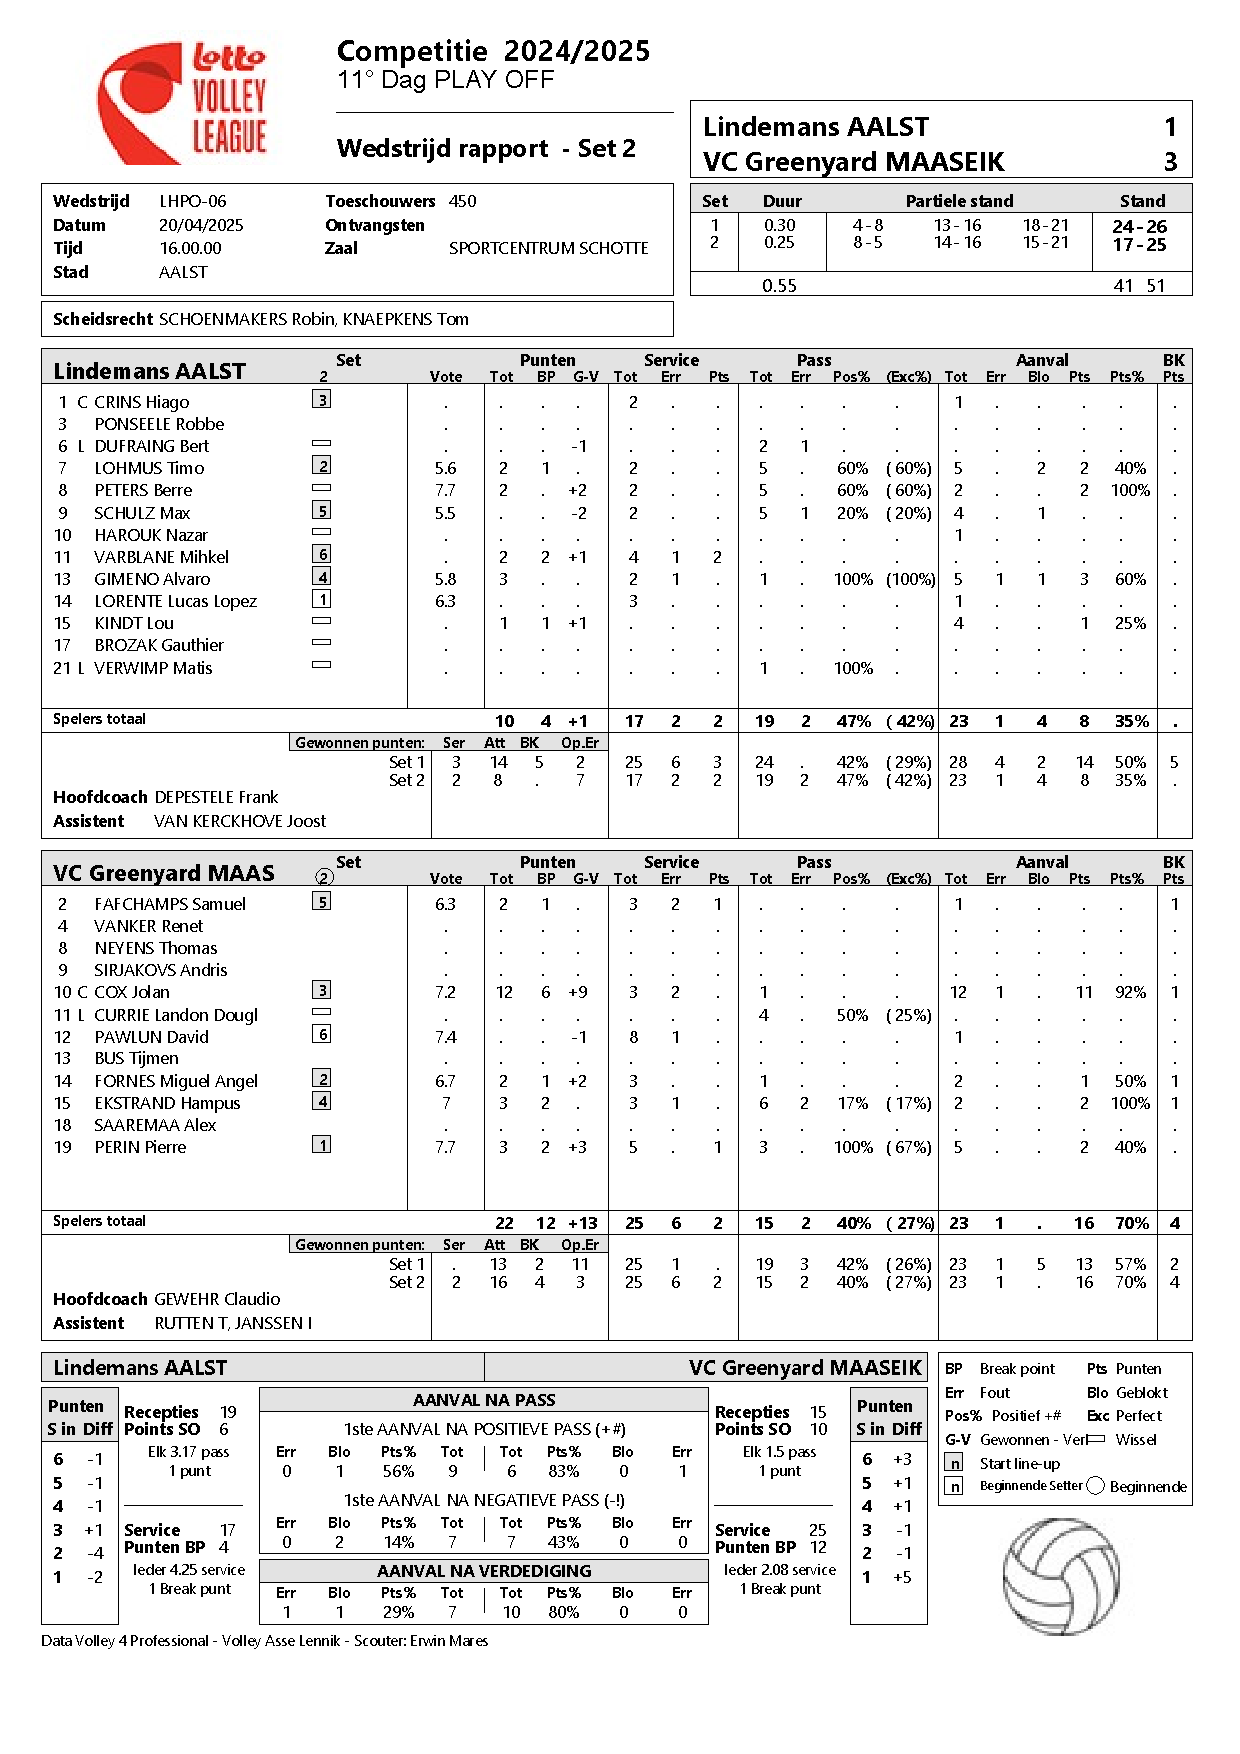
\includepdf[pages=-]{../inserts/20250420_LHPO06_aalst_maaseik_set2.pdf}
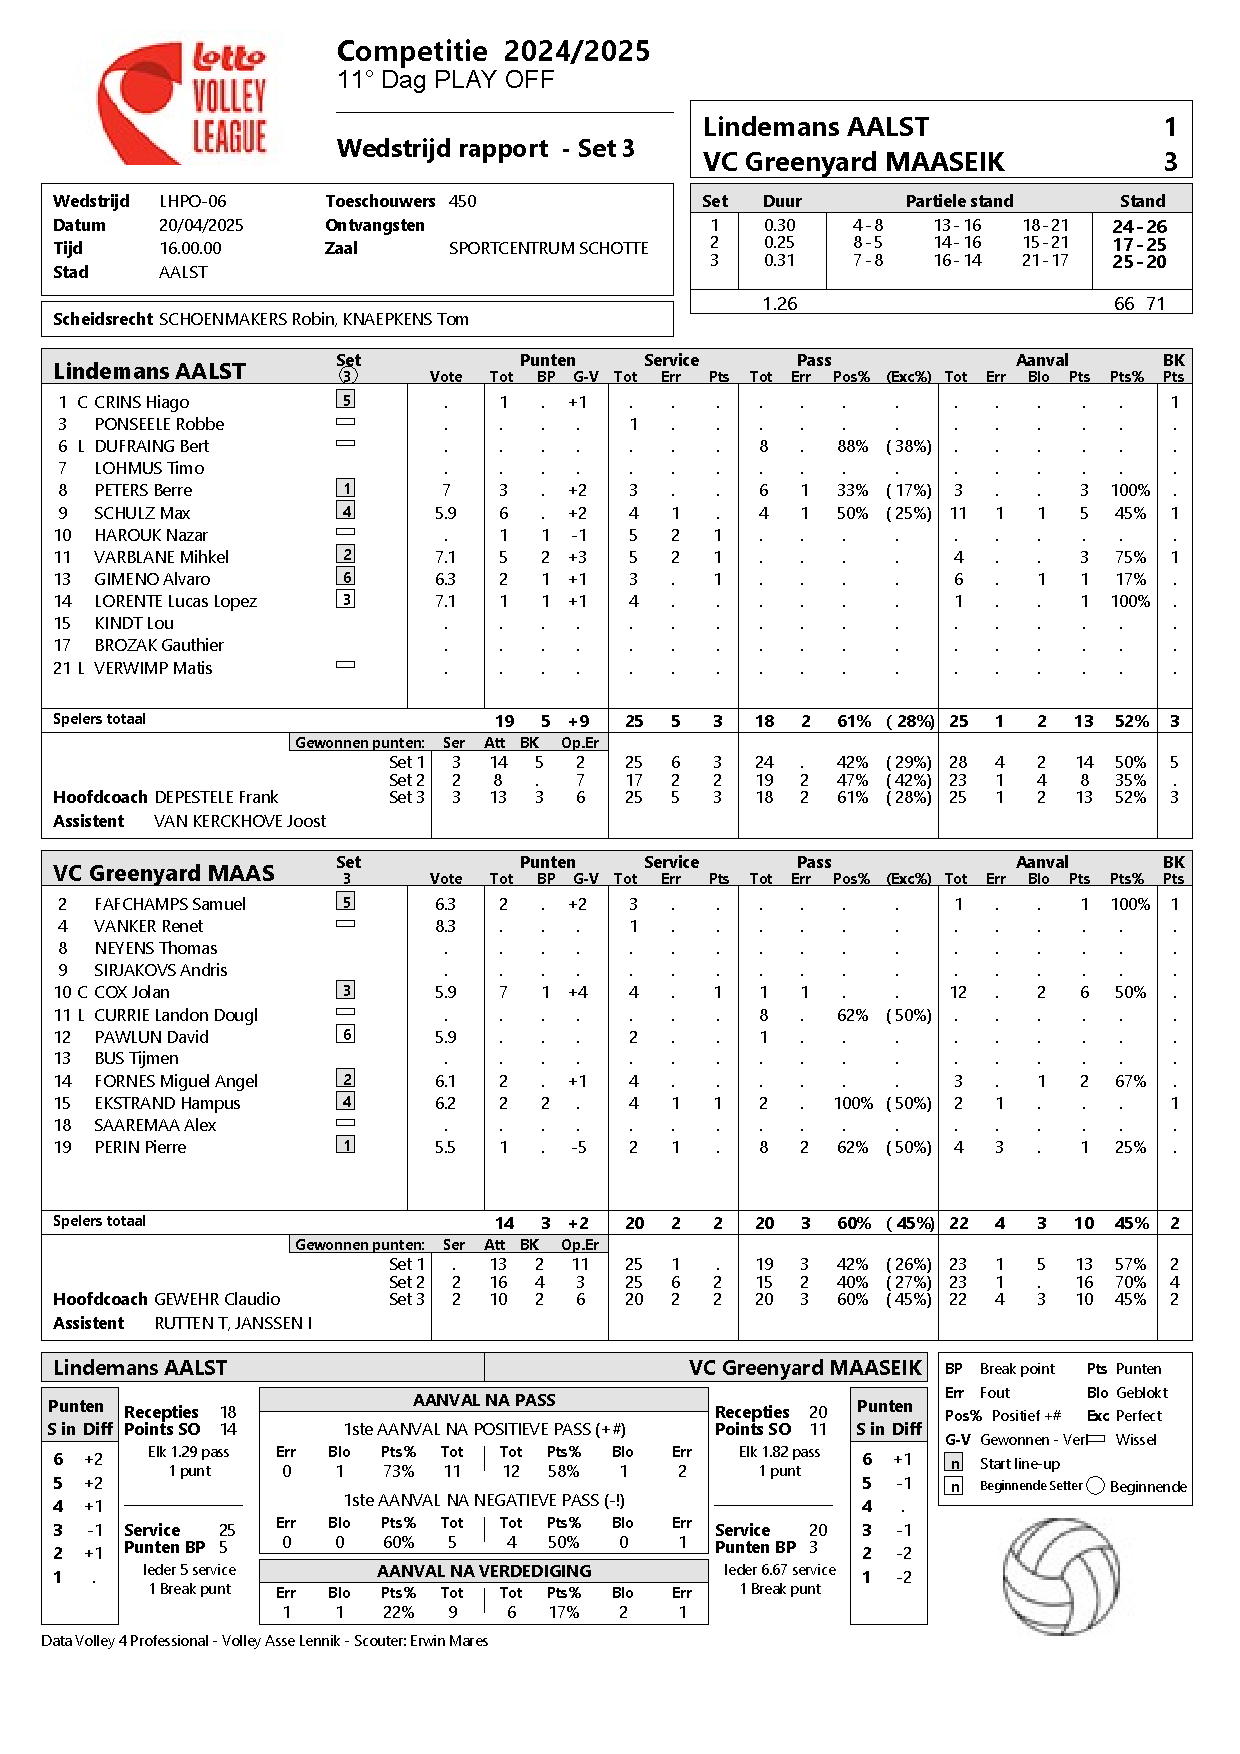
\includepdf[pages=-]{../inserts/20250420_LHPO06_aalst_maaseik_set3.pdf}
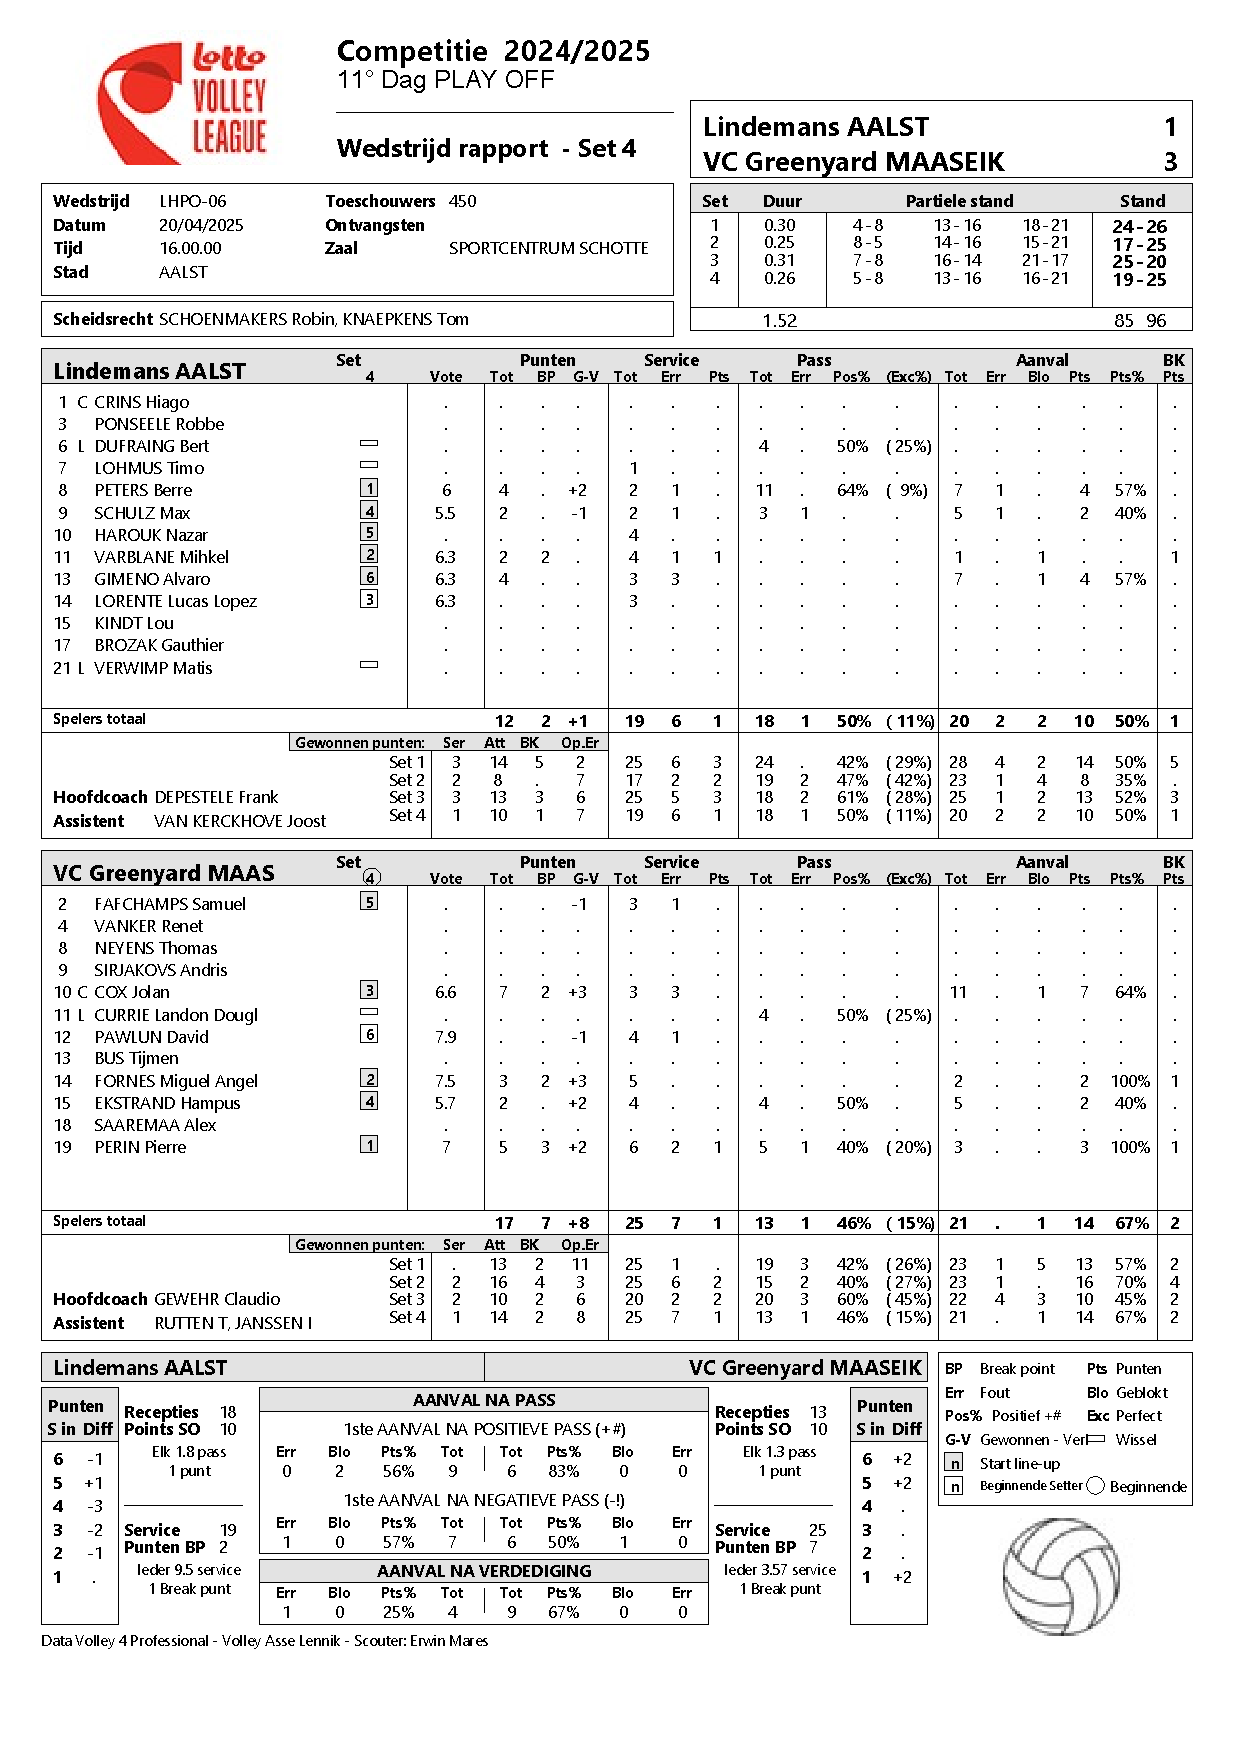
\includepdf[pages=-]{../inserts/20250420_LHPO06_aalst_maaseik_set4.pdf}

\chapter{Opslagsnelheden van de eerste wedstrijd}
De snelheden in deze bijlage zijn manueel verzameld en opgeschreven door de assistent-scouter van Lindemans Aalst tijdens de eerste wedstrijd. Ze vormen een belangrijk basis voor de vergelijkende studie van de snelheden in deze bachelorproef.

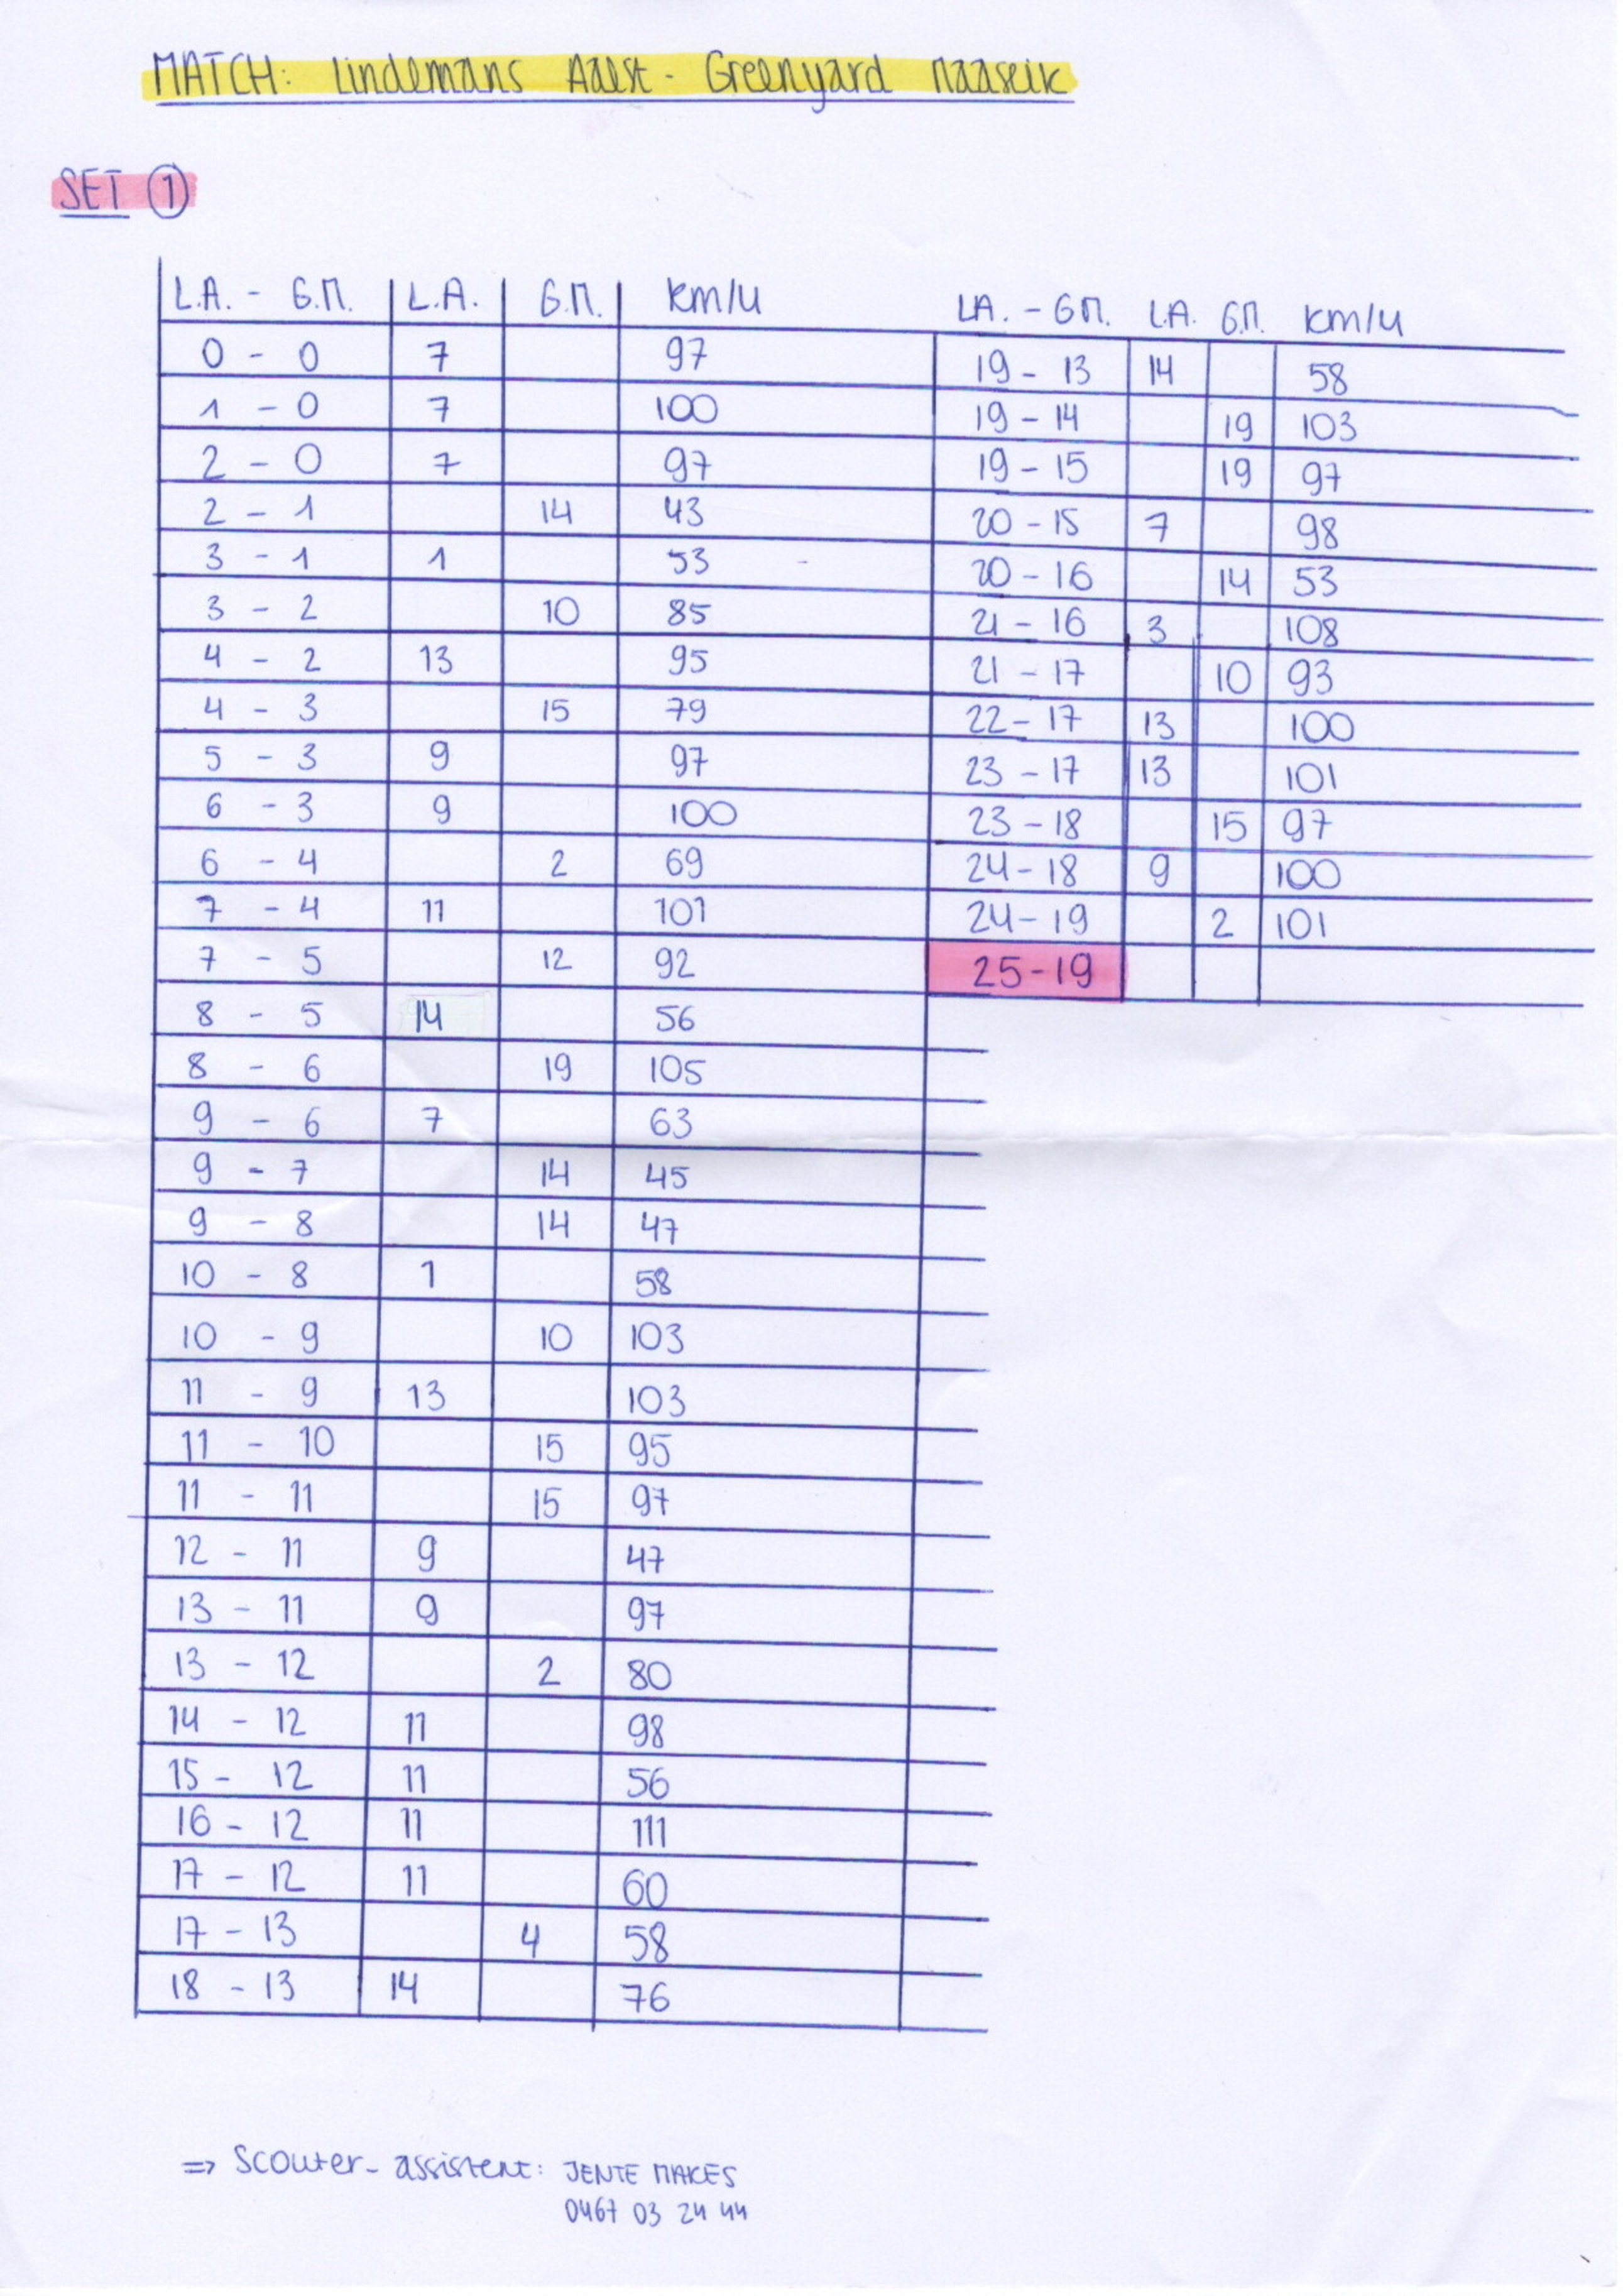
\includepdf[pages=-]{../inserts/Snelheden.pdf}

\chapter{Vergelijking van de AI- en manuele statistieken}
\label{ch:statistieken}
\section{Kwartfinale Play-offs - 16/4/2025}
\subsection{Vergelijking van de statistieken}
\subsubsection{Set 1 - Greenyard Maaseik}
\label{sec:PL1_Greenyard1}
Voor de opslagen van de eerste set van Greenyard Maaseik worden tabellen \ref{tab:PL1ServeMaaseikMan1} en \ref{tab:PL1ServeMaaseikAI1} bekeken. De beoordeling van de opslag is op een andere wijze gedaan dan bij de manuele invoer. Bij de manuele invoer wordt er gebruik gemaakt van tekens, terwijl bij de AI-invoer gebruik wordt gemaakt van cijfers. Bij de opslag komt het teken \# overeen met 0, + en / met 1, ! met 2, - en = met 3.

Hier valt op dat de goede opslagen door beide in deze set niet zijn genoteerd. De AI-invoer heeft de opslagen meer verdeeld onder score 1 en 2. Terwijl de manuele invoer enkel score 1 of 3 heeft gegeven. De scouter is dus kritischer in zijn beoordeling van de opslag.

\begin{table}[ht!]
    \centering
    \scriptsize
    \begin{tabular}{|l|c|c|c|c|c|c|c|c|c|}
      \hline
      \textbf{Speler} & *E\% & Tot & = & / & - & ! & + & \# \\ \hline
      Samuel Fafchamps & 0\% & 3 & 1 &  & 1 &  & 1 &  \\ 
      Renet Vancker & 0\% & 1 &  &  & 1 &  &  &  \\ 
      Jolan Cox  & 33\% & 3 & 1 &  &  &  & 2 &  \\ 
      Dawid Pawlun  & -100\% & 1 & 1 &  &  &  &  &  \\ 
      Miquel Angel Fornés & 75\% & 4 &  &  & 1 &  & 3 &  \\
      Hampus Ekstrand & 75\% & 4 &  & 1 & 1 &  & 2 &  \\
      Pierre Perin & 100\% & 3 &  &  &  &  & 3 &  \\ \hline
    \end{tabular}
    \caption[Manueel ingevoerde opslagstatistieken voor Greenyard Maaseik in set 1]{\label{tab:PL1ServeMaaseikMan1}Manueel ingevoerd opslag statistieken voor Greenyard Maaseik in set 1.}
\end{table}

\begin{table}[ht!]
  \centering
  \scriptsize
  \begin{tabular}{|l|c|c|c|c|c|c|c|c|c|c|c|c|} \hline
    \textbf{Speler} & SA & SE & TA & Pct & Eff & Rtg & 0 & 1 & 2 & 3 \\ \hline
    Samuel Fafchamps &  & 1 & 3 & 67 & -0.33 & 2.33 &  & 1 &  & 2  \\
    Renet Vancker &  &  & 1 & 100 & 0.00 & 3.00 &  &  &  & 1  \\
    Jolan Cox &  & 1 & 3 & 67 & -0.33 & 2.00 &  & 1 & 1 & 1 \\
    Dawid Pawlun &  & 1 & 1 & 0 & -1 & 3.00 &  &  &  & 1 \\
    Miquel Angel Fornés &  &  & 4 & 100 & 0.00 & 1.33 &  & 2 & 1 & \\
    Hampus Ekstrand &  &  & 4 & 100 & 0.00 & 1.00 &  & 3 &  & \\
    Pierre Perin &  &  & 3 & 100 & 0.00 & 1.33 &  & 2 & 1 & \\ \hline
  \end{tabular}
  \caption[Opslagstatistieken gemaakt door Balltime AI voor Greenyard Maaseik in set 1]{\label{tab:PL1ServeMaaseikAI1}Opslag statistieken gemaakt door Balltime AI voor Greenyard Maaseik in set 1.}
\end{table}

De recepties worden in tabellen \ref{tab:PL1ReceiveMaaseikMan1} en \ref{tab:PL1ReceiveMaaseikAI1} weergegeven. De manuele invoer heeft de recepties beoordeeld met de tekens \# overeen met 3, + en / met 2, ! met 1, - en = met 0.

Bij de receptie zijn er grote verschillen aanwezig tussen de manuele invoer en de AI-invoer. Er is één receptie van Landon Douglas Currie die door de AI-invoer niet kon beoordeeld worden, maar ook hier kan er geconstateerd worden dat de manuele invoer veel kritischer is in zijn beoordeling. 

\begin{table}[ht!]
    \centering
    \scriptsize
    \begin{tabular}{|l|c|c|c|c|c|c|c|c|c|}
        \hline
        \textbf{Speler} & *E\% & Tot & = & / & - & ! & + & \# \\ \hline
        Landon Douglas Currie & 38\% & 8 & 1 & 1 &  & 1 & 2 & 3 \\ 
        Hampus Ekstrand & 33\% & 3 &  &  &  & 2 & 1 &  \\ 
        Pierre Perin & 88\% & 8 &  &  &  & 1 & 2 & 5  \\ \hline
    \end{tabular}
    \caption[Manueel ingevoerde receptiestatistieken voor Greenyard Maaseik in set 1]{\label{tab:PL1ReceiveMaaseikMan1}Manueel ingevoerd receptie statistieken voor Greenyar Maaseik in set 1.}
\end{table}

\begin{table}[ht!]
  \centering
  \scriptsize
  \begin{tabular}{|l|c|c|c|c|c|c|c|c|c|} \hline
    \textbf{Speler} & 3 & 2 & 1 & 0 & TA & ? & Pass\% & Perfect PP\% & Good GP\% \\ \hline
    Thomas Neyens &  &  & 1 &  & 1 &  & 1.00 & 0 & 0  \\
    Landon Douglas Currie & 4 & 1 & 1 &  & 7 & 1 & 2.50 & 67 & 83 \\
    Hampus Ekstrand & 2 & 1 &  & 1 & 4 &  & 2.00 & 50 & 75 \\
    Pierre Perin & 5 & 1 & 2 &  & 8 &  & 2.38 & 62 & 75 \\ \hline
  \end{tabular}
  \caption[Receptie statistieken gemaakt door Balltime AI voor Greenyard Maaseik in set 1]{\label{tab:PL1ReceiveMaaseikAI1}Receptie statistieken gemaakt door Balltime AI voor Greenyard Maaseik in set 1.}
\end{table}

De spelverdeling wordt weergegeven in tabellen \ref{tab:PL1SetMaaseikMan1} en \ref{tab:PL1SetDigMaaseikAI1}. Over het algemeen zijn de hoeveelheden van de spelverdeling correct, bij één speler is er een verschil van 1 bij de AI-invoer. De kwaliteit van de set wordt bij de AI niet beoordeeld, waardoor geen verdere vergelijking mogelijk is.

Bij de verdeding, tabel \ref{tab:PL1DigMaaseikMan1} en \ref{tab:PL1SetDigMaaseikAI1}, zijn er duidelijke verschillen te zien. Dig Error (DE) komt overeen met een = bij de manuele invoer. Bij 2 spelers komt dit perfect overeen met de manuele invoer, bij de andere is er echter wel een verschil.  Zij hebben meer of minder verdedigingen gekregen door de AI.

\begin{table}[ht!]
    \centering
    \scriptsize
    \begin{tabular}{|l|c|c|c|c|c|c|c|c|c|}
        \hline
        \textbf{Speler}& *E\% & Tot & = & / & - & ! & + & \# \\ \hline
        Renet Vancker  & 100\% & 7 &  &  &  &  & 6 & 1  \\
        Jolan Cox  & 100\% & 1 &  &  &  &  & 1 &  \\ 
        Dawid Pawlun  & 100\% & 14 &  &  &  &  & 13 & 1  \\ 
        Pierre Perin & 100\% & 2 &  &  &  &  & 2 & \\ \hline
    \end{tabular}
    \caption[Manueel ingevoerde spelverdelingsstatistieken gemaakt voor Greenyard Maaseik in set 1]{\label{tab:PL1SetMaaseikMan1}Manueel ingevoerde spelverdeling statistieken gemaakt voor Greenyard Maaseik in set 1.}
\end{table}

\begin{table}[ht!]
    \centering
    \scriptsize
    \begin{tabular}{|l|c|c|c|c|c|c|c|c|c|}
        \hline
        \textbf{Speler}  & *E\% & Tot & = & / & - & ! & + & \# \\ \hline
        Jolan Cox & 0\% & 2 & 1 &  & 1 &  &  &  \\ 
        Landon Douglas Currie & 100\% & 1 &  &  &  &  & 1 &  \\ 
        Dawid Pawlun & 100\% & 1 &  &  &  &  & 1 &  \\ 
        Miquel Angel Fornés & 100\% & 1 &  &  &  &  & 1 &  \\ 
        Hampus Ekstrand & 0\% & 4 & 3 &  & 1 &  &  &  \\ 
        Pierre Perin & 50\% & 2 & 1 &  &  &  & 1 &  \\ \hline
    \end{tabular}
    \caption[Manueel ingevoerde verdedigingsstatistieken gemaakt voor Greenyard Maaseik in set 1]{\label{tab:PL1DigMaaseikMan1}Manueel ingevoerde verdediging statistieken gemaakt voor Greenyard Maaseik in set 1.}
\end{table}

\begin{table}[ht!]
  \centering
  \scriptsize
  \begin{tabular}{|l|c|c|c|c|c|c|c|}  \hline
    \textbf{Speler} & Ast & TA & SE & A/S & PCT & DS & DE \\ \hline
    Renet Vancker & 4 & 7 &  & 4.00 & 57 &  &  \\
    Thomas Neyens &  &  &  &  &  & 1 &  \\
    Jolan Cox &  & 1 &  & 0.00 & 0 & 1 & 1 \\
    Landon Douglas Currie &  &  &  &  &  & 1 &  \\
    Dawid Pawlun & 6 & 13 &  & 6.00 & 46 & 1 &  \\
    Miquel Angel Fornés &  &  &  &  &  & 1 & 1 \\
    Hampus Ekstrand &  &  &  &  &  & 3 & 1 \\
    Pierre Perin &  & 2 &  & 0.00 & 0 & 1 &  \\ \hline
  \end{tabular}
  \caption[Spelverdeling- en verdedigingsstatistieken gemaakt door Balltime AI voor Greenyard Maaseik in set 1]{\label{tab:PL1SetDigMaaseikAI1}Spelverdeling en verdediging statistieken gemaakt door Balltime AI voor Greenyard Maaseik in set 1.}
\end{table}

Bij de aanval (tabel \ref{tab:PL1AttMaaseikMan1} en \ref{tab:PL1AttBlockMaaseik1}) is het totaal aantal aanvallen gelijk bij iedereen behalve twee spelers. Zij hebben 1 en 2 aanvallen minder.

Bij de blokstatistieken (tabel \ref{tab:PL1BlockMaaseikMan1} en \ref{tab:PL1AttBlockMaaseik1}) wordt er op een volledig andere manier naar gekeken. De AI geeft statistieken waar de speler deel kan zijn van een éénmans- of een meermansblock. Dit is bij de manuele invoer niet het geval. Hierdoor geeft de AI dus eigenlijk ook geen blokpunten aan de spelers. Ookal is dit wel belangrijke informatie.

De aanvallen en blocks worden door de AI niet beoordeeld op kwaliteit.

\begin{table}[ht!]
    \centering
    \scriptsize
    \begin{tabular}{|l|c|c|c|c|c|c|c|c|c|}
        \hline
        \textbf{Speler} & *E\% & Tot & = & / & - & ! & + & \# \\ \hline
        Samuel Fafchamps & 75\% & 4 &  &  &  &  & 1 & 3 \\ 
        Jolan Cox & -20\% & 5 & 2 & 1 &  &  &  & 2 \\ 
        Dawid Pawlun  & 100\% & 2 & 1 &  &  &  &  & 2 \\ 
        Miquel Angel Fornés & 60\% & 5 &  &  &  &  & 2 & 3 \\
        Hampus Ekstrand & 25\% & 4 &  &  &  & 1 & 2 & 1 \\ 
        Pierre Perin & -17\% & 6 & 1 & 1 & 1 & 1 & 1 & 1 \\ \hline
    \end{tabular}
    \caption[Manueel ingevoerde aanvalsstatistieken gemaakt Greenyard Maaseik in set 1]{\label{tab:PL1AttMaaseikMan1}Manueel ingevoerde aanval statistieken gemaakt voor GreenyardMaaseik in set 1.}
\end{table}

\begin{table}[ht!]
    \centering
    \scriptsize
    \begin{tabular}{|l|c|c|c|c|c|c|c|c|c|}
        \hline
        \textbf{Speler} & *E\% & Tot & = & / & - & ! & + & \# \\ \hline
        Samuel Fafchamps & 0\% & 2 &  &  &  & 1 & 1 &  \\ 
        Jolan Cox & 100\% & 1 &  &  &  &  &  & 1 \\ 
        Dawid Pawlun & -100\% & 2 & 2 &  &  &  &  &  \\ 
        Hampus Ekstrand & 0\% & 2 & 1 &  &  &  &  & 1 \\ \hline
    \end{tabular}
    \caption[Manueel ingevoerde blokstatistieken gemaakt Greenyard Maaseik in set 1]{\label{tab:PL1BlockMaaseikMan1}Manueel ingevoerde blok statistieken gemaakt voor GreenyardMaaseik in set 1.}
\end{table}

\begin{table}[ht!]
  \centering
  \scriptsize
  \begin{tabular}{|l|c|c|c|c|c|c|c|c|c|c|c|} \hline
    \textbf{Speler} & K & E & TA & Atk\% & Kill\% & K/S & Error\% & BS & BA & BE \\ \hline
    Samuel Fafchamps & 3 &  & 4 & 0.75 & 75 & 3 & 0 &  &  & \\
    Jolan Cox & 2 & 3 & 6 & -0.17 & 33 & 2 & 50 & 1 &  &  \\
    Dawid Pawlun &   &   &   &   &   &   &   & 1 &  &   \\
    Miquel Angel Fornés & 3 &  & 5 & 0.60 & 6. & 3 &  & 1 & 1 & \\
    Hampus Ekstrand & 1 &  & 4 & 0.25 & 25 & 1 & 1 &  & 1 & \\
    Pierre Perin & 1 & 2 & 6 & -0.17 & 17 & 1 & 33 &  &   &  \\ \hline
    \end{tabular}
  \caption[Aanval en blokstatistieken gemaakt door Balltime AI voor Greenyard Maaseik in set 1]{\label{tab:PL1AttBlockMaaseik1}Aanval en blok statistieken gemaakt door Balltime AI voor Greenyard Maaseik in set 1.}
\end{table}

\subsubsection{Set 3 - Greenyard Maaseik}
\label{sec:PL1_Greenyard3}

Voor de opslagen worden tabellen \ref{tab:PL1ServeMaaseikMan3} en \ref{tab:PL1ServeMaaseikAI3} bekeken. De beoordeling van de opslag is op een andere wijze gedaan dan bij de manuele invoer. Bij de manuele invoer wordt er gebruik gemaakt van tekens, terwijl bij de AI-invoer gebruik wordt gemaakt van cijfers. Bij de opslag komt het teken \# overeen met 0, + en / met 1, ! met 2, - en = met 3.
Het aantal opslagen is bij beide hetzelfde getal. Ook de gemiste en perfecte opslagen zijn gelijk. De AI-invoer is echter veel minder kritisch dan de manuele invoer.

\begin{table}[ht!]
    \centering
    \scriptsize
    \begin{tabular}{|l|c|c|c|c|c|c|c|c|c|} \hline
        \textbf{Speler}& *E\% & Tot & = & / & - & ! & + & \#\\ \hline
        Samuel Fafchamps  & -33\% & 3 & 1 &  &  & 2 &  &  \\ 
        Jolan Cox  & -33\% & 3 & 2 &  & 1 &  &  &  \\ 
        Dawid Pawlun & 0\% & 2 &  &  & 2 &  &  &  \\
        Tijmen Bus & -100\% & 1 & 1 &  &  &  &  &  \\ 
        Miquel Angel Fornés & 100\% & 3 &  &  &  &  & 2 & 1 \\ 
        Hampus Ekstrand & 50\% & 2 &  &  & 1 &  &  & 1 \\ 
        Pierre Perin & 25\% & 4 & 1 &  & 1 &  &  & 2 \\ \hline
    \end{tabular}
    \caption[Manueel ingevoerde opslagstatistieken voor Greenyard Maaseik in set 3]{\label{tab:PL1ServeMaaseikMan3}Manueel ingevoerde opslagstatistieken voor Greenyard Maaseik in set 3.}
\end{table}

\begin{table}[ht!]
  \centering
  \scriptsize
  \begin{tabular}{|l|c|c|c|c|c|c|c|c|c|c|c|c|} \hline
    \textbf{Speler} & SA & SE & TA & Pct & Eff & Rtg & 0 & 1 & 2 & 3  \\ \hline
    Samuel Fafchamps &  & 1 & 3 & 67 & -0.33 & 2.33 &   &   & 2 & 1 \\
    Jolan Cox &  & 2 & 3 & 33 & -0.67 & 2.33 &   & 1 &   & 2 \\
    Dawid Pawlun &  &  & 2 & 100 & 0.00 & 1.50 &   & 1 & 1 &  \\
    Tijmen Bus &  & 1 & 1 & 0 & -1.00 & 3.00 &   & &   &  1 \\
    Miquel Angel Fornés & 1 &  & 3 & 100 & 0.33 & 1.33 & 1 & 1 &   & 1 \\
    Hampus Ekstrand & 1 &  & 2 & 100 & 0.50 & 1.00 & 1 &   & 1 &  \\
    Piere Perin & 2 & 1 & 4 & 75 & 0.25 & 1.5 & 2 &   &   & 2 \\ \hline
  \end{tabular}
  \caption[Opslagstatistieken gemaakt door Balltime AI voor Greenyard Maaseik in set 3]{\label{tab:PL1ServeMaaseikAI3}Opslagstatistieken gemaakt door Balltime AI voor Greenyard Maaseik in set 3.}
\end{table}

De recepties worden in tabellen \ref{tab:PL1ReceiveMaaseikMan3} en \ref{tab:PL1ReceiveMaaseikAI3} weergegeven. De manuele invoer heeft de recepties beoordeeld met de tekens \# overeen met 3, + en / met 2, ! met 1, - en = met 0. Op het eerste zicht valt op dat er een andere hoeveelheden recepties zijn geregisteerd bij sommige spelers. Opnieuw valt ook weer op dat de manuele invoer kritischer is dan de AI-invoer. Één opslag is ook niet gequoteerd geweest door de AI.

\begin{table}[ht!]
  \centering
  \scriptsize
  \begin{tabular}{|l|c|c|c|c|c|c|c|c|c|}
    \hline
    \textbf{Speler}& *E\% & Tot & = & / & - & ! & + & \#\\ \hline
    Andris Sirjakovs & 0\% & 2 &  &  &  & 2 &  &  \\ 
    Jolan Cox & -100\% & 1 &  & 1 &  &  &  &  \\
    Landon Douglas Currie & 60\% & 5 &  &  &  & 2 & 2 & 1 \\
    Tijmen Bus & -100\% & 1 &  & 1 &  &  &  &  \\ 
    Miquel Angel Fornés & 0\% & 1 &  &  & 1 &  &  &  \\ 
    Hampus Ekstrand & 17\% & 6 & 1 &  & 2 & 3 &  &  \\ 
    Pierre Perin & 29\% & 7 &  &  & 4 & 1 & 1 & 1 \\ \hline
  \end{tabular}
  \caption[Manueel ingevoerde receptiestatistieken voor Greenyard Maaseik in set 3]{\label{tab:PL1ReceiveMaaseikMan3}Manueel ingevoerde receptiestatistieken voor Greenyard Maaseik in set 3.}
\end{table}

\begin{table}[ht!]
  \centering
  \scriptsize
  \begin{tabular}{|l|c|c|c|c|c|c|c|c|c|} \hline
    \textbf{Speler} & 3 & 2 & 1 & 0 & TA & ? & Pass\% & Perfect PP\% & Good GP\% \\ \hline
    Andris Sirjakovs &  & 2 &  &  & 2 &  & 2 & 0 & 100 \\
    Landon Douglas Currie & 2 & 2 & 1 &  & 5 &  & 2.20 & 40 & 80 \\
    Tijmen Bus &  &  & 1 &  & 2 & 1 & 1.00 & 0 & 0 \\
    Miquel Angel Fornés &   &  & 1 &  & 1 &  & 1.00 & 0 & 0 \\
    Hampus Ekstrand &  & 2 & 3 & 1 & 6 &  & 1.17 & 0 & 33 \\
    Piere Perin & 1 & 1 & 4 &  & 6 &  & 1.50 & 17 & 33 \\ \hline
  \end{tabular}
  \caption[Receptiestatistieken gemaakt door Balltime AI voor Greenyard Maaseik in set 3]{\label{tab:PL1ReceiveMaaseikAI3}Receptiestatistieken gemaakt door Balltime AI voor Greenyard Maaseik in set 3.}
\end{table}

In tabellen \ref{tab:PL1SetMaaseikMan3} en \ref{tab:PL1SetDigMaaseikAI3} wordt de spelverdeling weergegeven. De hoeveelheden zijn hier zeer verschillend. Bij sommige spelers geeft de manuele invoer ze meer, bij andere dan weer meer door de AI. Volgens manuele invoer heeft Jolan Cox ook vijf keer aan spelverdeling gedaan, terwijl dit door AI geen enkele keer was. Dawid Pawlun heeft door de AI 17 keer aan spelverdeling gedaan, terwijl dit manueel maar 14 keer was. Dit is een verschil van 3. Dit is een groot verschil, maar het kan zijn dat de AI deze als spelverdeling heeft gezien, terwijl dit manueel niet zo was.

Ook bij de verdeding, tabel \ref{tab:PL1DigMaaseikMan3} en \ref{tab:PL1SetDigMaaseikAI3}, zijn er duidelijke verschillen te zien. Hier zijn er ook meerdere spelers die verschillende hoeveelheden verdedigingsacties hebben gekregen. Dit kan iets te maken hebben dat de verdediging buiten het beeld van de camera is gebeurd, waardoor de AI dit niet heeft kunnen registreren.

\begin{table}[ht!]
    \centering
    \scriptsize
    \begin{tabular}{|l|c|c|c|c|c|c|c|c|c|} \hline
        \textbf{Speler} & *E\% & Tot & = & / & - & ! & + & \# \\ \hline
        Samuel Fafchamps  & 100\% & 1 &  &  &  &  & 1 &  \\ 
        Renet Vancker & 100\% & 3 &  &  &  &  & 3 &  \\
        Jolan Cox & 100\% & 5 &  &  &  &  & 5 &  \\ 
        Landon Douglas Currie & 100\% & 1 &  &  &  &  & 1 &  \\ 
        Dawid Pawlun & 100\% & 14 &  &  &  &  & 11 & 3 \\ 
        Hampus Ekstrand & 100\% & 1 &  &  &  &  & 1 &  \\
        Pierre Perin & 100\% & 4 &  &  &  &  & 4 &  \\ \hline
    \end{tabular}
    \caption[Manueel ingevoerde spelverdelingsstatistieken voor Greenyard Maaseik in set 3]{\label{tab:PL1SetMaaseikMan3}Manueel ingevoerde spelverdeling statistieken voor Greenyard Maaseik in set 3.}
\end{table}

\begin{table}[ht!]
    \centering
    \scriptsize
    \begin{tabular}{|l|c|c|c|c|c|c|c|c|c|} \hline
        \textbf{Speler} & *E\% & Tot & = & / & - & ! & + & \#\\ \hline
        Renet Vancker & 0\% & 2 & 1 &  & 1 &  &  &  \\ 
        Jolan Cox & 75\% & 4 &  & 1 & 1 &  & 2 &  \\ 
        Landon Douglas Currie & 50\% & 2 &  &  & 1 &  & 1 &  \\ 
        Dawid Pawlun & 33\% & 3 &  &  & 2 &  & 1 &  \\ 
        Miquel Angel Fornés & 0\% & 2 & 1 &  & 1 &  &  &  \\ 
        Pierre Perin & 67\% & 3 &  &  & 1 &  & 2 &  \\ \hline
    \end{tabular}
    \caption[Manueel ingevoerde verdedigingsstatistieken voor Greenyard Maaseik in set 3]{\label{tab:PL1DigMaaseikMan3}Manueel ingevoerde verdediging statistieken voor Greenyard Maaseik in set 3.}
\end{table}

\begin{table}[ht!]
  \centering
  \scriptsize
  \begin{tabular}{|l|c|c|c|c|c|c|c|} \hline
    \textbf{Speler} & Ast & TA & SE & A/S & PCT & DS & DE \\ \hline
    Samuel Fafchamps &  & 1 &  & 0.00 & 0 &  &  \\
    Renet Vancker &  & 3 &  & 0.00 & 0 & 1 &  \\
    Jolan Cox &  &  &  &  &  & 5 &  \\
    Landon Douglas Currie &  & 2 &  & 0.00 & 0 & 3 & 1 \\
    Dawid Pawlun & 6 & 17 &  & 6.00 & 35 & 4 &  \\
    Tijmen Bus &  & 1 &  & 0.00 & 0 & 1 &  \\
    Hampus Ekstrand & 1 & 2 &  & 1.00 & 50 &  &  \\
    Piere Perin &  & 5 &  & 0.00 & 0 & 2 &  \\  \hline
  \end{tabular}
  \caption[Spelverdelings- en verdedigingsstatistieken gemaakt door Balltime AI voor Greenyard Maaseik in set 3]{\label{tab:PL1SetDigMaaseikAI3}Spelverdelings- en verdedigingsstatistieken gemaakt door Balltime AI voor Greenyard Maaseik in set 3.}
\end{table}

Tabel \ref{tab:PL1AttMaaseikMan3}, \ref{tab:PL1BlockMaaseikMan3} en \ref{tab:PL1AttBlockMaaseikAI3} tonen de de aanval en blokstatistieken gemaakt door de AI en de manuele invoer voor Greenyard Maaseik in set 3. 

De aanvallen worden correct geregisteerd door de AI, behalve bij één speler. Jolan Cox heeft een aanval te minder dan bij de manuele invoer. 

De aanvallen en blokkeringen worden door de AI niet beoordeeld op kwaliteit. Ook worden de blokkeringen op een totaal andere manier bekeken door de AI. Dit systeem geeft geen duidelijke blokpunten. Dit is echter wel van belang.

\begin{table}[ht!]
    \centering
    \scriptsize
    \begin{tabular}{|l|c|c|c|c|c|c|c|c|c|} \hline
        \textbf{Speler} & *E\% & Tot & = & / & - & ! & + & \#\\ \hline
        Andris Sirjakovs & -67\% & 3 &  & 2 &  &  & 1 &  \\ 
        Jolan Cox & 0\% & 5 &  & 1 & 3 &  &  & 1 \\ 
        Dawid Pawlun & 0\% & 2 & 1 &  &  &  &  & 1 \\ 
        Tijmen Bus & -25\% & 4 & 1 & 1 &  & 1 &  & 1 \\ 
        Miquel Angel Fornés & 50\% & 2 &  &  &  &  & 1 & 1 \\ 
        Hampus Ekstrand & 12\% & 8 & 1 & 1 & 1 & 1 & 1 & 3 \\ 
        Pierre Perin  & 17\% & 6 & 1 &  & 2 & 1 &  & 2 \\ \hline
    \end{tabular}
   \caption[Manueel ingevoerde aanvalsstatistieken voor Greenyard Maaseik in set 3]{\label{tab:PL1AttMaaseikMan3}Manueel ingevoerde aanvalsstatistieken voor Greenyard Maaseik in set 3.}
\end{table}

\begin{table}[ht!]
    \centering
    \scriptsize
    \begin{tabular}{|l|c|c|c|c|c|c|c|c|c|} \hline
        \textbf{Speler} & *E\% & Tot & = & / & - & ! & + & \#\\ \hline
        Samuel Fafchamps & 50\% & 2 &  &  &  & 1 &  & 1 \\ 
        Jolan Cox & -100\% & 1 & 1 &  &  &  &  &  \\
        Dawid Pawlun & -25\% & 4 & 1 & 1 &  &  & 1 & 1 \\
        Miquel Angel Fornés & 0\% & 3 & 1 &  &  & 1 &  & 1 \\ 
        Pierre Perin & 0\% & 1 &  &  &  & 1 &  &  \\ \hline
    \end{tabular}
    \caption[Manueel ingevoerde blokstatistieken voor Greenyard Maaseik in set 3]{\label{tab:PL1BlockMaaseikMan3}Manueel ingevoerde blokstatistieken voor Greenyard Maaseik in set 3.}
\end{table}

\begin{table}[ht!]
  \centering
  \scriptsize
  \begin{tabular}{|l|c|c|c|c|c|c|c|c|c|c|c|} \hline
    \textbf{Speler} &  K & E & TA & Atk\% & Kill\% & K/S & Error\% & BS & BA & BE & B/S \\ \hline
    Samuel Fafchamps &   &   &   &   &   &   &   & 1 &  & & 1.00 \\
    Andris Sirjakovs &  & 2 & 3 & -0.67 & 0 &  & 67 &   &  &  & \\
    Jolan Cox & 1 & 1 & 6 & 0.00 & 17 & 1 & 17 &  &  &  & \\
    Dawid Pawlun & 1 & 1 & 2 & 0.00 & 50 & 1 & 50 & 1 &  &  & 1.00 \\
    Tijmen Bus &  & 2 & 4 & -0.50 & 0 &  & 50 & &  &  &  \\
    Miquel Angel Fornés & 1 &  & 2 & 0.50 & 50 & 1 & 0 & 1 & & & 1.00 \\
    Hampus Ekstrand & 3 & 1 & 8 & 0.25 & 38 & 3 & 12 &   &   &  & \\
    Piere Perin & 2 & 1 & 6 & 0.17 & 33 & 2 & 17 &  &  & &  \\ \hline
  \end{tabular}
  \caption[Aanvals- en blokstatistieken gemaakt door Balltime AI voor Greenyard Maaseik in set 3]{\label{tab:PL1AttBlockMaaseikAI3}Aanvals- en blokstatistieken gemaakt door Balltime AI voor Greenyard Maaseik in set 3.}
\end{table}

\subsection{Vergelijking van de opslagsnelheden}
\label{sec:snelheden}

In tabellen \ref{tab:PL1ServeMan1}, \ref{tab:PL1ServeMan2} en \ref{tab:PL1ServeMan3} zijn de manueel gemeten opslagsnelheden weergegeven. In \ref{tab:PL1ServeAI1}, \ref{tab:PL1ServeAI2} en \ref{tab:PL1ServeAI3} zijn  de opslagsnelheden weergegeven gemaakt door Balltime AI. De eerste kolom geeft de setstanden aan. De tweede kolom geeft de speler van Lindemans Aalst aan die serveert. De derde kolom geeft de speler van Greenyard Maaseik aan die serveert en de vierde kolom geeft de snelheid in km/u aan. Op figuur \ref{fig:PL1_Serve} is een voorbeeld van de opslagmeting van Balltime AI te zien. De snelheid is weergegeven in de rechterbovenhoek van het scherm.

\begin{figure}
  \centering
  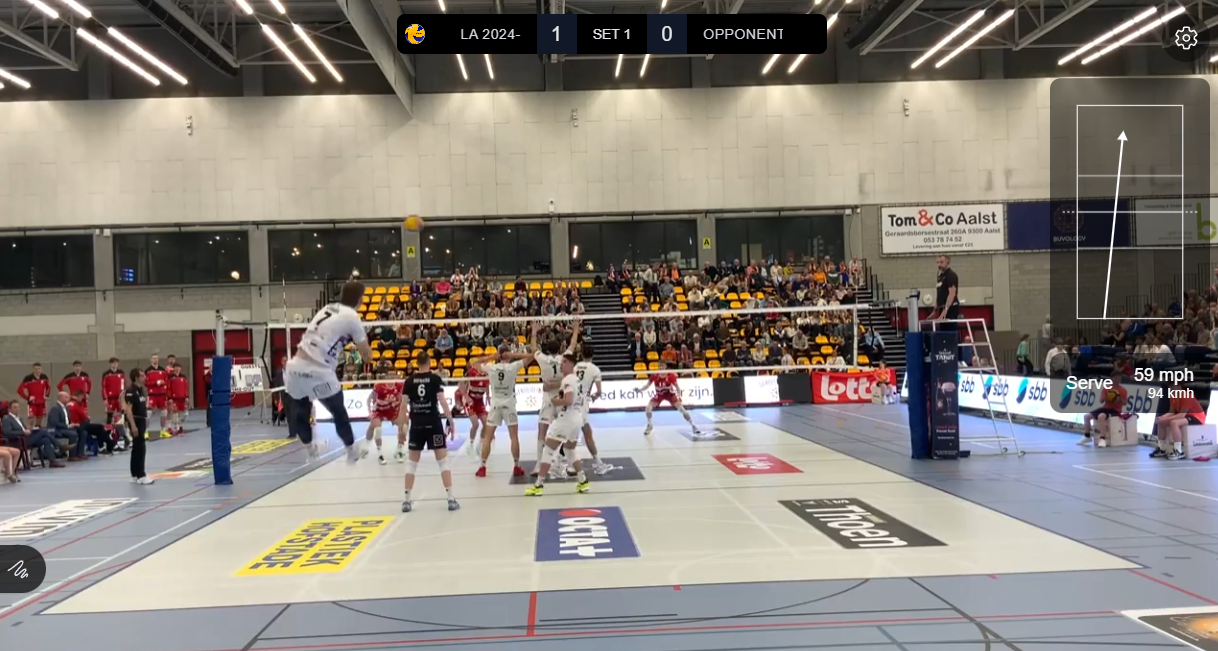
\includegraphics[width=\textwidth]{PL1_AM/opslag.png}
  \caption{\label{fig:PL1_Serve}Voorbeeld van opslagmeting van Balltime AI.}
\end{figure}

In set 1 valt op dat Balltime AI niet alle snelheden heeft opgemeten, zoals te zien is in tabel \ref{tab:PL1ServeAI1}. Er zijn maar 13 metingen gedaan terwijl er 44 opslagen zijn geweest, ongeveer een 29,55\%. Dit kan te maken hebben met het feit dat de camera niet altijd goed gericht was op de bal, waardoor de snelheid niet correct kon worden gemeten. Er zijn ook grote verschillen aanwezig in de gemeten snelheden. Een verklaring hiervoor kan zijn dat bij de manuele meting het toestel naar een geel object zoekt, idealiter de bal, maar de tribune van Lindemans Aalst is ook geel. Dit zorgt ervoor dat de snelheden soms incorrect gemeten worden. 
Balltime AI registreerde sommige snelheden aanzienlijk hoger of lager dan de manuele metingen. Bij stand 3-2 mat Balltime AI 111 km/u, terwijl de manuele meting 85 km/u aangaf. Bij 12-11 gaf de AI 109 km/u, tegenover slechts 47 km/u bij de manuele meting.

\begin{table}[ht!]
  \centering
  \scriptsize
  \begin{tabular}{|c|c|c|c|} \hline
    L.A.-G.M. & L.A. & G.M. & km/u \\ \hline
    0-0 & 7 & & 97 \\
    1-0 & 7 & & 100 \\
    2-0 & 7 & & 97 \\
    2-1 & & 14 & 43 \\
    3-1 & 1 & & 53 \\
    3-2 & & 10 & 85 \\
    4-2 & 13 & & 95 \\
    4-3 & & 15 & 79 \\
    5-3 & 9 & & 97 \\
    6-3 & 9 & & 100 \\
    6-4 & & 2 & 69 \\
    7-4 & 11 & & 101 \\
    7-5 & & 12 & 92 \\
    8-5 & 14 & & 56 \\
    8-6 & & 19 & 105 \\
    9-6 & 7 & & 63 \\
    9-7 & & 14 & 45 \\
    9-8 & & 14 & 47 \\
    10-8 & 1 & & 58 \\
    10-9 & & 10 & 103 \\
    11-9 & 13 & & 103 \\
    11-10 & & 15 & 95 \\
    11-11 & & 15 & 97 \\
    12-11 & 9 & & 47 \\
    13-11 & 9 & & 97 \\
    13-12 & & 2 & 80 \\
    14-12 & 11 & & 98 \\
    15-12 & 11 & & 56 \\
    16-12 & 11 & & 111 \\
    17-12 & 11 & & 60 \\
    17-13 & & 4 & 58 \\
    18-13 & 14 & & 76 \\
    19-13 & 14 & & 58 \\
    19-14 & & 19 & 103 \\
    19-15 & & 19 & 97 \\
    20-15 & 7 & & 98 \\
    20-16 & & 14 & 53 \\
    21-16 & 3 & & 108 \\
    21-17 & & 10 & 93 \\
    22-17 & 13 & & 100 \\
    23-17 & 13 & & 101 \\
    23-18 & & 15 & 97 \\
    24-18 & 9 & & 100 \\
    24-19 & & 2 & 101 \\
    25-19 & & & \\ \hline
  \end{tabular}
  \caption[Manueel gemeten opslagsnelheden tijdens set 1]{\label{tab:PL1ServeMan1}Manueel gemeten opslagsnelheden tijdens set 1.}
\end{table}

\begin{table}[ht!]
  \centering
  \scriptsize
  \begin{tabular}{|c|c|c|c|} \hline
    L.A.-G.M. & L.A. & G.M. & km/u \\ \hline
    0-0 & 7 & & - \\
    1-0 & 7 & & - \\
    2-0 & 7 & & - \\
    2-1 & & 14 & 48 \\
    3-1 & 1 & & - \\
    3-2 & & 10 & 111 \\
    4-2 & 13 & & 89 \\
    4-3 & & 15 & - \\
    5-3 & 9 & & - \\
    6-3 & 9 & & - \\
    6-4 & & 2 & 120 \\
    7-4 & 11 & & - \\
    7-5 & & 12 & - \\
    8-5 & 14 & & - \\
    8-6 & & 19 & - \\
    9-6 & 7 & & - \\
    9-7 & & 14 & 52 \\
    9-8 & & 14 & - \\
    10-8 & 1 & & 61 \\
    10-9 & & 10 & - \\
    11-9 & 13 & & 62 \\
    11-10 & & 15 & 122 \\
    11-11 & & 15 & 98 \\
    12-11 & 9 & & 109 \\
    13-11 & 9 & & - \\
    13-12 & & 2 & 92 \\
    14-12 & 11 & & - \\
    15-12 & 11 & & - \\
    16-12 & 11 & & - \\
    17-12 & 11 & & - \\
    17-13 & & 4 & 60 \\
    18-13 & 14 & & - \\
    19-13 & 14 & & - \\
    19-14 & & 19 & - \\
    19-15 & & 19 & - \\
    20-15 & 7 & & - \\
    20-16 & & 14 & 54 \\
    21-16 & 3 & & - \\
    21-17 & & 10 & - \\
    22-17 & 13 & & - \\
    23-17 & 13 & & - \\
    23-18 & & 15 & - \\
    24-18 & 9 & & - \\
    24-19 & & 2 & - \\
    25-19 & & & \\ \hline
  \end{tabular}
  \caption[Gemeten opslagsnelheden door Balltime AI tijdens set 1]{\label{tab:PL1ServeAI1}Gemeten opslagsnelheden door Balltime AI tijdens set 1.}
\end{table}

Ook in de tweede set, zie tabel \ref{tab:PL1ServeAI2}, valt op dat Balltime AI niet alle snelheden heeft opgemeten. In deze set zijn er 23 metingen gedaan van de 46 opslagen, 50\% van de opslagen. Dit is een verbetering ten opzichte van de eerste set, maar er zijn nog steeds veel snelheden die niet zijn gemeten. De snelheden die wel zijn gemeten, zijn ook hier weer verschillend van de manueel gemeten snelheden. Bij stand 10-9 werd manueel 80 km/u gemeten, terwijl Balltime AI 114 km/u registreerde. Een kleinere afwijking was dan wel weer te vinden bij stand 16-13, waar Balltime AI een snelheid van 41 km/u aangaf tegenover 45 km/u bij de manuele meting. Balltime AI gaf op sommige momenten wel veel hogere waardes, zoals 122 km/u bij 13-11, waar manueel slechts 55 km/u werd gemeten. In deze set lijken er ook enkele consistentere snelheden te zijn gemeten, zoals bij 1-0, waar manueel de meting 93 km/u aangaf en Balltime AI 94 km/u aangaf.

\begin{table}[ht!]
  \centering
  \scriptsize
  \begin{tabular}{|c|c|c|c|} \hline
    L.A.-G.M. & L.A. & G.M. & km/u \\ \hline
    0-0 &  & 19 & 116 \\
    1-0 & 7 & & 93 \\
    1-1 &  & 14 & 50 \\
    2-1 & 1 & & 51 \\
    3-1 & 1 & & 53 \\
    3-2 &  & 10 & 95 \\
    4-2 & 13 & & 89 \\
    4-3 &  & 15 & 71 \\
    5-3 & 9 & & 97 \\
    5-4 &  & 2 & 90 \\
    6-4 & 11 & & 82 \\
    6-5 &  & 4 & 61 \\
    7-5 & 14 & & 53 \\
    7-6 &  & 19 & 116 \\
    8-6 & 7 &  & 101 \\
    8-7 &  & 14 & 55 \\
    8-8 &  & 14 & 58 \\
    9-8 & 7 & & 60 \\
    9-9 &  & 10 & 106 \\
    10-9 & 13 & & 80 \\
    11-9 & 13 & & 95 \\
    12-9 & 13 & & 97 \\
    12-10 &  & 15 & 109 \\
    12-11 &  & 15 & 92 \\
    13-11 & 9 &  & 55 \\
    13-12 &  & 2 & 93 \\
    14-12 & 11 &  & 98 \\
    14-13 &  & 4 & 53 \\
    15-13 & 14 &  & 51 \\
    16-13 & 14 &  & 45 \\
    16-14 &  & 19 & 114 \\
    17-14 & 7 &  & 105 \\
    18-14 & 7 &  & 100 \\
    18-15 &  & 14 & 50 \\
    18-16 &  & 14 & 58 \\
    19-16 & 3 &  & 106 \\
    20-16 & 3 &  & 98 \\
    20-17 &  & 10 & 105 \\
    21-17 & 13 &  & 97 \\
    22-17 & 13 &  & 106 \\
    23-17 & 13 &  & 100 \\
    23-18 &  & 15 & 58 \\
    23-19 &  & 15 & 79 \\
    24-19 & 9 &  & 98 \\
    24-20 &  & 2 & 108 \\
    24-21 &  & 2 & 101 \\
    25-21 &  &  &  \\ \hline
  \end{tabular}
  \caption[Manueel gemeten opslagsnelheden tijdens set 2]{\label{tab:PL1ServeMan2}Manueel gemeten opslagsnelheden tijdens set 2.}
\end{table}

\begin{table}[ht!]
  \centering
  \scriptsize
  \begin{tabular}{|c|c|c|c|} \hline
    L.A.-G.M. & L.A. & G.M. & km/u \\ \hline
    0-0 &  & 19 & - \\
    1-0 & 7 & & 94 \\
    1-1 &  & 14 & 56 \\
    2-1 & 1 & & 55 \\
    3-1 & 1 & & 59 \\
    3-2 &  & 10 & - \\
    4-2 & 13 & & - \\
    4-3 &  & 15 & - \\
    5-3 & 9 & & - \\
    5-4 &  & 2 & 95 \\
    6-4 & 11 & & - \\
    6-5 &  & 4 & - \\
    7-5 & 14 & & 71 \\
    7-6 &  & 19 & - \\
    8-6 & 7 &  & 70 \\
    8-7 &  & 14 & 54 \\
    8-8 &  & 14 & 43 \\
    9-8 & 7 & & 73 \\
    9-9 &  & 10 & 92 \\
    10-9 & 13 & & 114 \\
    11-9 & 13 & & 109 \\
    12-9 & 13 & & 98 \\
    12-10 &  & 15 & - \\
    12-11 &  & 15 & 74 \\
    13-11 & 9 &  & 122 \\
    13-12 &  & 2 & - \\
    14-12 & 11 &  & - \\
    14-13 &  & 4 & 52 \\
    15-13 & 14 &  & 113 \\
    16-13 & 14 &  & 41 \\
    16-14 &  & 19 & - \\
    17-14 & 7 &  & - \\
    18-14 & 7 &  & 53 \\
    18-15 &  & 14 & 49 \\
    18-16 &  & 14 & - \\
    19-16 & 3 &  & - \\
    20-16 & 3 &  & - \\
    20-17 &  & 10 & - \\
    21-17 & 13 &  & 118 \\
    22-17 & 13 &  & - \\
    23-17 & 13 &  & - \\
    23-18 &  & 15 & - \\
    23-19 &  & 15 & - \\
    24-19 & 9 &  & 33 \\
    24-20 &  & 2 & - \\
    24-21 &  & 2 & - \\
    25-21 &  &  &  \\ \hline
  \end{tabular}
  \caption[Gemeten opslagsnelheden door Balltime AI tijdens set 2]{\label{tab:PL1ServeAI2}Gemeten opslagsnelheden door Balltime AI tijdens set 2.}
\end{table}

Tijdens de laatste set zijn er het minste aantal metingen gedaan door Balltime AI, zie tabel \ref{tab:PL1ServeAI3}. In deze set zijn er maar 10 metingen gedaan van de 43 opslagen, slechts 23,3\%. Dit is een grote daling ten opzichte van de vorige sets. De snelheden die wel zijn gemeten liggen wel dichter bij de manuele metingen, buiten enkele uitschieters. Een verschil van 40 km/u bij stand 15-11 tussen de manuele metingen van 106 km/u en de AI meting van 66 km/u is wel opmerkelijk. Ook bij stand 24-17 is er een groot verschil. Balltime AI gaf hier een snelheid aan van 125 km/u, terwijl de manuele meting slechts 103 km/u aangaf.

\begin{table}[ht!]
  \centering
  \scriptsize
  \begin{tabular}{|c|c|c|c|} \hline
    L.A.-G.M. & L.A. & G.M. & km/u \\ \hline
    0-0 & 7 & & 61 \\
    1-0 & 7 & & 89 \\
    2-0 & 7 & & 103 \\
    3-0 & 7 & & 105 \\
    4-0 & 7 & & 108 \\
    5-0 & 7 & & 98 \\
    5-1 & & 14 & 56 \\
    5-2 & & 14 & 53 \\
    6-2 & 1 & & 58 \\
    6-3 & & 10 & 60 \\
    6-4 & & 10 & 103 \\
    7-4 & 13 & & 93 \\
    7-5 &  & 13 & 56 \\
    8-5 & 9 & & 92 \\
    8-6 &  & 2 & 97 \\
    9-6 & 11 & & 60 \\
    10-6 & 11 & & 105 \\
    11-6 & 11 & & 101 \\
    11-7 & & 12 & 84 \\
    12-7 & 14 & & 55 \\
    13-7 & 14 & & 50 \\
    13-8 & & 19 & 100 \\
    13-9 & & 19 & 100 \\
    14-9 & 7 & & 103 \\
    14-10 & & 14 & 56 \\
    15-10 & 1 & & 60 \\
    15-11 & & 10 & 106 \\
    16-11 & 13 & & 98 \\
    17-11 & 13 & & 114 \\
    18-11 & 13 & & 111 \\
    19-11 & 13 & & 113 \\
    20-11 & 13 & & 69 \\
    21-11 & 13 & & 92 \\
    21-12 & & 15 & 76 \\
    21-13 & & 15 & 69 \\
    22-13 & 9 & & 97 \\
    22-14 & & 2 & 69 \\
    22-15 & & 2 & 71 \\
    23-15 & 11 & & 68 \\
    23-16 & & 12 & 84 \\
    24-16 & 14 & & 53 \\
    24-17 & & 19 & 103 \\
    24-18 & & 19 & 101 \\
    25-18 & & & \\ \hline
  \end{tabular}
  \caption[Manueel gemeten opslagsnelheden tijdens set 3]{\label{tab:PL1ServeMan3}Manueel gemeten opslagsnelheden tijdens set 3.}
\end{table}

\begin{table}[ht!]
  \centering
  \scriptsize
  \begin{tabular}{|c|c|c|c|} \hline
    L.A.-G.M. & L.A. & G.M. & km/u \\ \hline
    0-0 & 7 & & - \\
    1-0 & 7 & & - \\
    2-0 & 7 & & - \\
    3-0 & 7 & & - \\
    4-0 & 7 & & - \\
    5-0 & 7 & & - \\
    5-1 & & 14 & 44 \\
    5-2 & & 14 & 44 \\
    6-2 & 1 & & 52 \\
    6-3 & & 10 & - \\
    6-4 & & 10 & - \\
    7-4 & 13 & & - \\
    7-5 &  & 13 & - \\
    8-5 & 9 & & - \\
    8-6 &  & 2 & - \\
    9-6 & 11 & & - \\
    10-6 & 11 & & - \\
    11-6 & 11 & & - \\
    11-7 & & 12 & - \\
    12-7 & 14 & & - \\
    13-7 & 14 & & - \\
    13-8 & & 19 & - \\
    13-9 & & 19 & - \\
    14-9 & 7 & & - \\
    14-10 & & 14 & 50 \\
    15-10 & 1 & & 59 \\
    15-11 & & 10 & 66 \\
    16-11 & 13 & & - \\
    17-11 & 13 & & - \\
    18-11 & 13 & & - \\
    19-11 & 13 & & - \\
    20-11 & 13 & & - \\
    21-11 & 13 & & - \\
    21-12 & & 15 & - \\
    21-13 & & 15 & - \\
    22-13 & 9 & & 113 \\
    22-14 & & 2 & 78 \\
    22-15 & & 2 & - \\
    23-15 & 11 & & - \\
    23-16 & & 12 & - \\
    24-16 & 14 & & - \\
    24-17 & & 19 & 125 \\
    24-18 & & 19 & 105 \\
    25-18 & & & \\ \hline
  \end{tabular}
  \caption[Gemeten opslagsnelheden door Balltime AI tijdens set 3]{\label{tab:PL1ServeAI3}Gemeten opslagsnelheden door Balltime AI tijdens set 3.}
\end{table}

\section{Kwartfinale Play-offs - 20/4/2025}
\subsection{Vergelijking van de statistieken}
\subsubsection{Set 1 - Greenyard Maaseik}
\label{sec:PL3_Greenyard1}

% TODO: tekst - stats OK

\begin{table}[ht!]
    \centering
    \scriptsize
    \begin{tabular}{|l|c|c|c|c|c|c|c|c|c|} \hline
        \textbf{Speler} & *E\% & Tot & = & / & - & ! & + & \# \\ \hline
        Samuel Fafchamps & 20\% & 5 &  & & 4 &  & 1 &  \\ 
        Jolan Cox & 100\% & 7 &  & 1 &  & & 6 &  \\ 
        Dawid Pawlun & 50\% & 4 &  &  & 2 & & 2 &  \\
        Miquel Angel Fornés & 33\% & 3 &  & & 2 &  & 1 &  \\
        Hampus Ekstrand & 0\% & 4 & 1 &  & 2 &  & 1 & \\ 
        Pierre Perin & 100\% & 2 &  &  &  & & 2 &  \\ \hline
    \end{tabular}
    \caption[Manueel ingevoerde opslagstatistieken voor Greenyard Maaseik in set 1]{\label{tab:PL3ServeMaaseikMan1}Manueel ingevoerde opslagstatistieken voor Greenyard Maaseik in set 1.}
\end{table}

\begin{table}[ht!]
  \centering
  \scriptsize
  \begin{tabular}{|l|c|c|c|c|c|c|c|c|c|c|c|} \hline
    \textbf{Speler} & SA & SE & TA & Pct & Eff & Rtg & 0 & 1 & 2 & 3 \\ \hline
    Samuel Fafchamps &  &  & 5 & 100 & 0.00 & 2.20 &   & 1 & 2 & 2 \\
    Jolan Cox &  &  & 8 & 100 & 0.00 & 1.67 &   & 3 & 2 & 1 \\
    Dawid Pawlun &  &  & 4 & 100 & 0.00 & 1 .00 &   & 4 &  & 0 \\
    Miquel Angel Fornés &  &  & 3 & 100 & 0.00 & 2.00 &  & 1 & 1 & 1 \\
    Hampus Ekstrand &  & 1 & 4 & 75 & -0.25 & 2.50 &   & & 2 & 2 \\
    Pierre Perin & & & 2 & 100 & 0.00 & 1.00 &   & 1 &   &  \\  \hline
  \end{tabular}
  \caption[Opslagstatistieken gemaakt door Balltime AI voor Greenyard Maaseik in set 1]{\label{tab:PL3ServeMaaseikAI1}Opslagstatistieken gemaakt door Balltime AI voor Greenyard Maaseik in set 1.}
\end{table}

% TODO: tekst - stats OK

\begin{table}[ht!]
    \centering
    \scriptsize
    \begin{tabular}{|l|c|c|c|c|c|c|c|c|c|} \hline
        \textbf{Speler} & *E\% & Tot & = & / & - & ! & + & \# \\ \hline
        Thomas Neyens & -100\% & 2 & 1 & 1 &  &  & & \\
        Landon Douglas Currie & 43\% & 7 & 1 &  & 2 & & 1 & 3 \\ 
        Dawid Pawlun & 0\% & 1 &  &  & 1 &  &  & \\ 
        Hampus Ekstrand & 40\% & 5 &  &  & 1 & 2 & 1 & 1 \\ 
        Pierre Perin & 25\% & 4 & 1 &  & 1 & & 1 & 1 \\ \hline
    \end{tabular}
    \caption[Manueel ingevoerde receptiestatistieken voor Greenyard Maaseik in set 1]{\label{tab:PL3ReceiveMaaseikMan1}Manueel ingevoerde receptiestatistieken voor Greenyar Maaseik in set 1.}
\end{table}

\begin{table}[ht!]
  \centering
  \scriptsize
    \begin{tabular}{|l|c|c|c|c|c|c|c|c|c|} \hline
    \textbf{Speler} & 3 & 2 & 1 & 0 & TA & ? & Pass\% & Perfect PP\% & Good GP\% \\ \hline
    Landon Douglas Currie & 3 & 1 & 2 &   & 6 &  & 2.17 & 5 & 67 \\
    Dawid Pawlun &  &  & 1 &  & 1 &  & 1.00 & 0 & 0 \\
    Hampus Ekstrand & 1 & 2 & 1 & & 5 & 1 & 2.00 & 25 & 75 \\
    Pierre Perin & 2 & 1 &  & 1 & 4 & & 2.00 & 50 & 75 \\  \hline
  \end{tabular}
  \caption[Receptiestatistieken gemaakt door Balltime AI voor Greenyard Maaseik in set 1]{\label{tab:PL3ReceiveMaaseikAI1}Receptiestatistieken gemaakt door Balltime AI voor Greenyard Maaseik in set 1.}
\end{table}

% TODO: tekst - stats OK

\begin{table}[ht!]
    \centering
    \scriptsize
    \begin{tabular}{|l|c|c|c|c|c|c|c|c|c|} \hline
        \textbf{Speler} & *E\% & Tot & = & / & - & ! & + & \# \\ \hline
        Jolan Cox & 100\% & 2 &  &  &  &  & 2 &  \\ 
        Dawid Pawlun & 88\% & 17 &  & 1 &  &  & 11 & 5 \\ 
        Miquel Angel Fornés & 100\% & 1 &  &  &  &  & 1 &  \\ 
        Hampus Ekstrand & 100\% & 3 &  &  &  &  & 3 &  \\ \hline
    \end{tabular}
    \caption[Manueel ingevoerde spelverdelingsstatistieken gemaakt voor Greenyard Maaseik in set 1]{\label{tab:PL3SetMaaseikMan1}Manueel ingevoerde spelverdelingsstatistieken gemaakt voor Greenyard Maaseik in set 1.}
\end{table}

\begin{table}[ht!]
    \centering
    \scriptsize
    \begin{tabular}{|l|c|c|c|c|c|c|c|c|c|} \hline
        \textbf{Speler} & *E\% & Tot & = & / & - & ! & + & \# \\ \hline
        Jolan Cox & 100\% & 1 &  & 1 &  &  &  & \\
        Landon Douglas Currie & 25\% & 4 & 2 &  & 1 &  & 1 & \\ 
        Dawid Pawlun & 100\% & 1 &  &  &  &  & 1 & \\
        Pierre Perin & 0\% & 2 &  &  & 2 &  &  &  \\ \hline
    \end{tabular}
    \caption[Manueel ingevoerde verdedigingsstatistieken gemaakt voor Greenyard Maaseik in set 1]{\label{tab:PL3DigMaaseikMan1}Manueel ingevoerde verdedigingsstatistieken gemaakt voor Greenyard Maaseik in set 1.}
\end{table}

\begin{table}[ht!]
  \centering
  \scriptsize
  \begin{tabular}{|l|c|c|c|c|c|c|c|} \hline
    \textbf{Speler} & Ast & TA & SE & A/S & PCT & DS & DE \\ \hline
    Jolan Cox & 1 & 2 &  & 1.00 & 50 & 1 & 0 \\
    Landon Douglas Currie &  &  &  &   &   & 3 &   \\
    Dawid Pawlun & 9 & 16 &  & 9.00 & 60 & 1 & 0 \\
    Miquel Angel Fornés & 1 & 2 &  & 1.00 & 50 & 1 & 1 \\
    Hampus Ekstrand &  & 2 &  & 0.00 & 0 & 1 & \\
    Pierre Perin &   &   &   &   &   & 2 &   \\ \hline
  \end{tabular}
  \caption[Spelverdelings- en verdedigingsstatistieken gemaakt door Balltime AI voor Greenyard Maaseik in set 1]{\label{tab:PL3SetDigMaaseikAI1}Spelverdelings- en verdedigingsstatistieken gemaakt door Balltime AI voor Greenyard Maaseik in set 1.}
\end{table}

% TODO: tekst - stats OK

\begin{table}[ht!]
    \centering
    \scriptsize
    \begin{tabular}{|l|c|c|c|c|c|c|c|c|c|} \hline
        \textbf{Speler} & *E\% & Tot & = & / & - & ! & + & \# \\ \hline
        Samuel Fafchamps & 0\% & 2 &  & 1 &  &  &  & 1 \\ 
        Jolan Cox & 20\% & 5 & 1 & 1 &  &  &  & 3 \\ 
        Miquel Angel Fornés & 100\% & 2 &  &  &  &  &  & 2 \\ 
        Hampus Ekstrand & 0\% & 2 &  & 1 &  &  &  & 1 \\ 
        Pierre Perin & 33\% & 12 &  & 2 &  & 2 & 2 & 6 \\ \hline
    \end{tabular}
    \caption[Manueel ingevoerde aanvalsstatistieken gemaakt Greenyard Maaseik in set 1]{\label{tab:PL3AttMaaseikMan1}Manueel ingevoerde aanvalsstatistieken gemaakt voor GreenyardMaaseik in set 1.}
\end{table}

\begin{table}[ht!]
    \centering
    \scriptsize
    \begin{tabular}{|l|c|c|c|c|c|c|c|c|c|} \hline
        \textbf{Speler} & *E\% & Tot & = & / & - & ! & + & \# \\ \hline
        Samuel Fafchamps & -100\% & 2 & 2 &  &  &  &  & \\ 
        Dawid Pawlun & -20\% & 5 & 1 & 1 & 2 & & & 1 \\ 
        Miquel Angel Fornés & -20\% & 5 & 1 & 1 &  & 2 & & 1 \\
        Pierre Perin & 0\% & 1 &  &  & 1 &  &  &\\ \hline
    \end{tabular}
    \caption[Manueel ingevoerde blokstatistieken gemaakt Greenyard Maaseik in set 1]{\label{tab:PL3BlockMaaseikMan1}Manueel ingevoerde blokstatistieken gemaakt voor GreenyardMaaseik in set 1.}
\end{table}

\begin{table}[ht!]
  \centering
  \scriptsize
    \begin{tabular}{|l|c|c|c|c|c|c|c|c|c|c|c|} \hline
    \textbf{Speler} & K & E & TA & Atk\% & Kill\% & K/S & Error\% & BS & BA & BE & B/S \\ \hline
    Samuel Fafchamps & 1 & 1 & 2 & 0.00 & 50 & 1 & 50 &  &  &  & \\
    Jolan Cox & 3 & 2 & 5 & 0.20 & 60 & 3 & 40 &   &  &  &  \\
    Dawid Pawlun &   &   &   &   &   &   &   & 1 & 1 & & 1.00\\
    Miquel Angel Fornés & 2 &  & 2 & 1.00 & 100 & 2 & 0 & 1 & 2 & & 1.00\\
    Hampus Ekstrand & 2 &  & 2 & 1.00 & 100 & 2 & 0 &  & & & \\
    Pierre Perin & 5 & 2 & 11 & 0.27 & 45 & 5 & 18 & 0 & 1 &  & 0.00\\ \hline
  \end{tabular}
  \caption[Aanvals- en blokstatistieken gemaakt door Balltime AI voor Greenyard Maaseik in set 1]{\label{tab:PL3AttBlockMaaseik1}Aanvals- en blokstatistieken gemaakt door Balltime AI voor Greenyard Maaseik in set 1.}
\end{table}
    
\subsubsection{Set 2 - Lindemans Aalst}
\label{sec:PL3_Aalst2}
% TODO: vergelijking
% TODO: andere stats ook bijzetten
\begin{figure}
  \centering
  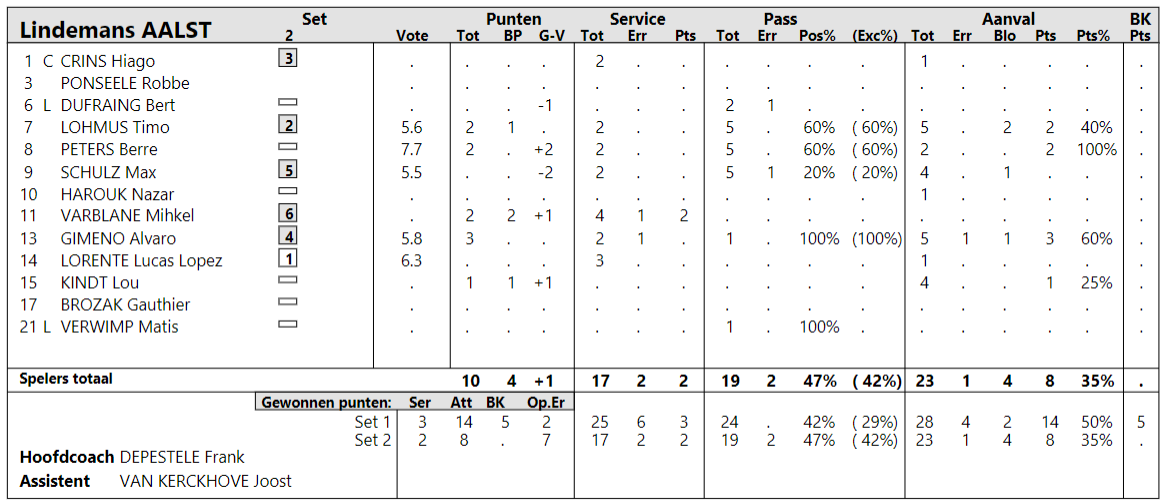
\includegraphics[width=\textwidth]{PL3_AM/SET2/PL3_AM_2.png}
  \caption{\label{fig:PL3_AM_2}Resultaten van de manuele invoer van Lindemans Aalst in set 2.}
\end{figure}

\begin{table}[ht!]
  \centering
  \scriptsize
  \begin{tabular}{|l|c|c|c|c|c|c|c|c|c|c|c|} \hline
    \textbf{Name} & SA & SE & TA & Pct & Eff & Rtg & 0 & 1 & 2 & 3 & ? \\ \hline
    Timo Lohmus & 0 & 0 & 1 & 1 & 0 & 2 &   & 1 &   & 0 &   \\
    Berre Peeters & 0 & 1 & 2 & 0.5 & -0.5 & 2.5 &   & 1 & 1 & 0 & 6 \\
    Max Schulz & 0 & 1 & 2 & 0.5 & -0.5 & 2.5 &   & 1 & 1 & 0 &   \\
    Nezar Harouk & 0 & 0 & 4 & 1 & 0 & 2.25 &   & 1 & 1 & 2 & 0 \\
    Mihkel Varblane & 1 & 1 & 4 & 0.75 & 0 & 1.33 & 1 & 1 &   & 1 & 0 \\
    Alvaro Gimeno Rubio & 0 & 3 & 3 & 0 & -1 & 3 &   &   & 3 & 0 &   \\
    Lucas Lorente López & 0 & 0 & 3 & 1 & 0 & 2 &   & 1 &   & 0 &   \\
    Bert Dufraing &   &   &   &   &   &   & 2 & 1 & 1 &   &   \\
    Matis Verwimp &   &   &   &   &   &   &   &   &   &   &   \\
    Lindemans Aalst & 1 & 7 & 25 & 0.72 & -0.24 & 2.36 & 1 & 4 & 5 & 15 & 0 \\
    Greenyard Maaseik & 1 & 6 & 19 & 0.68 & -0.26 & 2.25 & 1 & 2 & 5 & 8 & 0 \\ \hline
  \end{tabular}
  \caption[Serve statistieken gemaakt door Balltime AI voor Lindemans Aalst in set 2]{\label{tab:PL3ServeAalst2}Serve statistieken gemaakt door Balltime AI voor Lindemans Aalst in set 2.}
\end{table}

\begin{table}[ht!]
  \centering
  \scriptsize
  \begin{tabular}{|l|c|c|c|c|c|c|c|c|c|} \hline
    \textbf{Name} & 3 & 2 & 1 & 0 & TA & ? & Pass\% & Perfect PP\% & Good GP\% \\ \hline
    Timo Lohmus &   &   &   &   &   &   &   &   &   \\
    Berre Peeters & 4 & 2 &   & 12 & 12 & 0 & 2.33 & 0.5 & 0.83 \\
    Max Schulz &   & 1 &   & 1 & 1 & 0 & 0 & 0 & 0 \\
    Nezar Harouk &   &   &   &   &   &   &   &   &   \\
    Mihkel Varblane &   &   &   &   &   &   &   &   &   \\
    Alvaro Gimeno Rubio &   &   &   &   &   &   &   &   &   \\
    Lucas Lorente López &   &   &   &   &   &   &   &   &   \\
    Bert Dufraing & 2 & 1 & 1 &   & 4 & 0 & 2.25 & 0.5 & 0.75 \\
    Matis Verwimp &   &   &   &   &   &   &   &   &   \\
    Lindemans Aalst & 2 & 5 & 2 &   & 12 & 3 & 2 & 0.22 & 0.78 \\
    Greenyard Maaseik & 8 & 5 & 4 &   & 17 & 0 & 2.24 & 0.47 & 0.76 \\ \hline
  \end{tabular}
  \caption[Receive statistieken gemaakt door Balltime AI voor Lindemans Aalst in set 2]{\label{tab:PL3ReceiveAalst2}Receive statistieken gemaakt door Balltime AI voor Lindemans Aalst in set 2.}
\end{table}

\begin{table}[ht!]
  \centering
  \scriptsize
  \begin{tabular}{|l|c|c|c|c|c|c|c|} \hline
    \textbf{Name} & Set Ast & Set TA & Set SE & A/S & PCT & Dig DS & Dig DE \\ \hline
    Timo Lohmus &   &   &   &   &   &   &   \\
    Berre Peeters &   &   &   &   &   &   &   \\
    Max Schulz & 0 & 2 & 0 & 0 & 0 &   &   \\
    Nezar Harouk &   &   &   &   &   &   &   \\
    Mihkel Varblane &   &   &   &   &   &   &   \\
    Alvaro Gimeno Rubio &   &   &   &   &   &   &   \\
    Lucas Lorente López & 10 & 16 & 0 & 10 & 0.62 & 1 & 0 \\
    Bert Dufraing & 1 & 0 & 0 & 1 & 0 & 1 & 0 \\
    Matis Verwimp & 0 & 1 & 0 & 0 & 0 &   &   \\
    Lindemans Aalst & 12 & 19 & 0 & 12 & 0.63 & 9 & 1 \\
    Greenyard Maaseik & 10 & 20 & 0 & 10 & 0.5 & 5 & 0 \\ \hline
  \end{tabular}
  \caption[Setting en digging statistieken gemaakt door Balltime AI voor Lindemans Aalst in set 2]{\label{tab:PL3SetDigAalst2}Setting en digging statistieken gemaakt door Balltime AI voor Lindemans Aalst in set 2.}
\end{table}

\begin{table}[ht!]
  \centering
  \scriptsize
  \begin{tabular}{|l|c|c|c|c|c|c|c|c|c|} \hline
    \textbf{Name} & Attack K & E & TA & Atk\% & Kill\% & K/S & Error\% & Block BS & BA \\ \hline
    Timo Lohmus &   &   &   &   &   &   &   &   &   \\
    Berre Peeters & 1 & 7 & 4 & 1 & 0.57 & 4 & 0.14 &   &   \\
    Max Schulz & 2 & 1 & 5 & 0.2 & 0.4 & 2 & 0.2 &   &   \\
    Nezar Harouk &   &   &   &   &   &   &   &   &   \\
    Mihkel Varblane & 0 & 1 & 1 & -1 & 0 & 0 & 1 & 1 & 0 \\
    Alvaro Gimeno Rubio & 4 & 1 & 7 & 0.43 & 0.57 & 4 & 0.14 &   &   \\
    Lucas Lorente López & 0 & 0 & 1 & 0 & 0 & 0 & 0 & 0 & 0 \\
    Bert Dufraing &   &   &   &   &   &   &   &   &   \\
    Matis Verwimp &   &   &   &   &   &   &   &   &   \\
    Lindemans Aalst & 14 & 1 & 21 & 0.62 & 0.67 & 14 & 0.05 &   &   \\
    Greenyard Maaseik & 10 & 4 & 21 & 0.29 & 0.48 & 10 & 0.19 & 1 & 0 \\ \hline
  \end{tabular}
  \caption[Attacking en blocking statistieken gemaakt door Balltime AI voor Lindemans Aalst in set 2]{\label{tab:PL3AttBlockAalst2}Attacking en blocking statistieken gemaakt door Balltime AI voor Lindemans Aalst in set 2.}
\end{table}

\begin{figure}
  \centering
  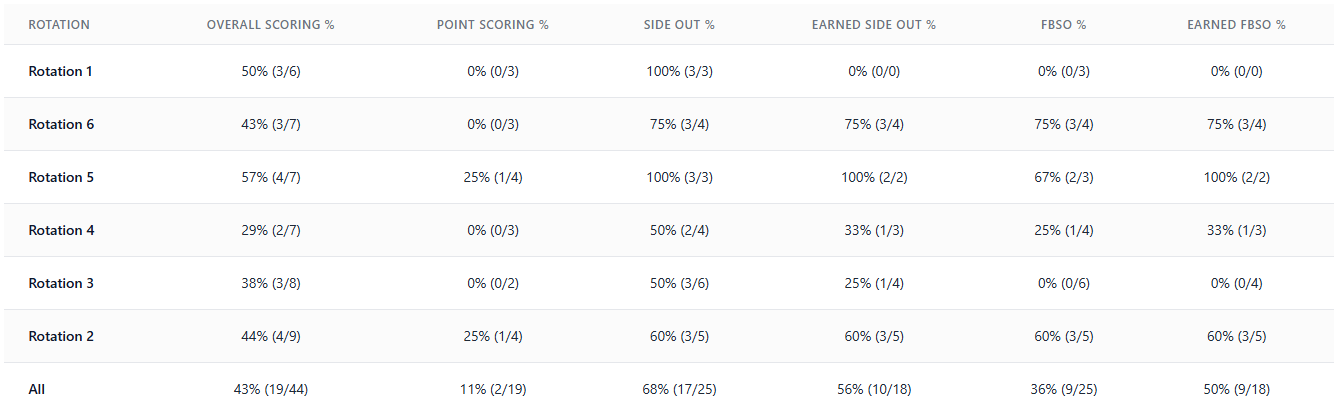
\includegraphics[width=\textwidth]{PL3_AM/SET2/ROT_STATS.png}
  \caption{\label{fig:PL3_ROT_STATS_2}Rotatie statistieken gemaakt door Balltime AI voor Lindemans Aalst in set 2.}
\end{figure}
\subsubsection{Set 3 - Greenyard Maaseik}
\label{sec:PL3_Greenyard3}

% TODO: tekst - stats OK

\begin{table}[ht!]
    \centering
    \scriptsize
    \begin{tabular}{|l|c|c|c|c|c|c|c|c|c|} \hline
        \textbf{Speler} & *E\% & Tot & = & / & - & ! & + & \#\\ \hline
        Samuel Fafchamps & 0\% & 3 &  &  & 3 &  &  &  \\ 
        Renet Vancker & 0\% & 1 &  &  & 1 &  &  & \\ 
        Jolan Cox & 25\% & 4 &  &  & 3 &  &  & 1 \\ 
        Dawid Pawlun & 50\% & 2 &  &  & 1 &  & 1 &  \\ 
        Miquel Angel Fornés & 25\% & 4 &  &  & 3 &  & 1 &  \\ 
        Hampus Ekstrand & 50\% & 4 & 1 &  &  &  & 2 & 1 \\ 
        Pierre Perin & 0\% & 2 & 1 &  &  &  & 1 &  \\ \hline
    \end{tabular}
    \caption[Manueel ingevoerde opslagstatistieken voor Greenyard Maaseik in set 3]{\label{tab:PL3ServeMaaseikMan3}Manueel ingevoerde opslagstatistieken voor Greenyard Maaseik in set 3.}
\end{table}

\begin{table}[ht!]
  \centering
  \scriptsize
  \begin{tabular}{|l|c|c|c|c|c|c|c|c|c|c|c|} \hline
    \textbf{Speler} & SA & SE & TA & Pct & Eff & Rtg & 0 & 1 & 2 & 3 \\ \hline
    Samuel Fafchamps &  &  & 3 & 100 & 0.00 & 2.67 &   &  & 1 & 2  \\
    Renet Vancker &  &  & 1 & 100 & 0.00 & 3.00 &  &  &  & 1 \\
    Jolan Cox & 1 &  & 4 & 100 & 0.25 & 1.50 & 1 & 1 & 1 & 1 \\
    Dawid Pawlun &  &  & 2 & 100 & 0.00 & 3.00 &   &   & & 1 \\
    Miquel Angel Fornés & 1 & 1 & 4 & 75 & 0.00 & 2.00 &   & 1 & 2 & 1 \\
    Hampus Ekstrand & 1 & 1 & 4 & 75 & 0.00 & 1.50 & 1 & 1 & 1 & 1\\
    Pierre Perin & & 1 & 2 & 50 & -0.50 & 2.5 &   &  & 1 & 1 \\ \hline
  \end{tabular}
  \caption[Opslagstatistieken gemaakt door Balltime AI voor Greenyard Maaseik in set 3]{\label{tab:PL3ServeMaaseikAI3}Opslag statistieken gemaakt door Balltime AI voor Greenyard Maaseik in set 3.}
\end{table}

% TODO: tekst - stats OK

\begin{table}[ht!]
    \centering
    \scriptsize
    \begin{tabular}{|l|c|c|c|c|c|c|c|c|c|} \hline
        \textbf{Speler} & *E\% & Tot & = & / & - & ! & + & \#\\ \hline
        Jolan Cox & -100\% & 1 & 1 &  &  &  &  & \\ 
        Landon Douglas Currie & 62\% & 8 &  &  & 1 & 2 & 1 & 4 \\ 
        Dawid Pawlun & -100\% & 1 &  & 1 &  &  &  &  \\ 
        Hampus Ekstrand & 100\% & 2 &  &  &  &  & 1 & 1 \\ 
        Pierre Perin & 38\% & 8 & 2 &  & 1 &  & 1 & 4 \\ \hline
    \end{tabular}
    \caption[Manueel ingevoerde receptiestatistieken voor Greenyard Maaseik in set 3]{\label{tab:PL3ReceiveMaaseikMan3}Manueel ingevoerde receptiestatistieken voor Greenyard Maaseik in set 3.}
\end{table}

\begin{table}[ht!]
  \centering
  \scriptsize
  \begin{tabular}{|l|c|c|c|c|c|c|c|c|c|} \hline
    \textbf{Speler} & 3 & 2 & 1 & 0 & TA & Pass\% & Perfect PP\% & Good GP\% \\ \hline
    Landon Douglas Currie & 3 & 3 & 2 &  & 8 & 2.12 & 38 & 75 \\
    Hampus Ekstrand & 1 & 1 &   & 2 & & 1.5 & 0 & 50 \\
    Pierre Perin & 6 & 1 &   & 2 & 9 & 2.22 & 67 & 78 \\ \hline
  \end{tabular}
  \caption[Receptiestatistieken gemaakt door Balltime AI voor Greenyard Maaseik in set 3]{\label{tab:PL3ReceiveMaaseikAI3}Receptiestatistieken gemaakt door Balltime AI voor Greenyard Maaseik in set 3.}
\end{table}

% TODO: tekst - stats OK

\begin{table}[ht!]
    \centering
    \scriptsize
    \begin{tabular}{|l|c|c|c|c|c|c|c|c|c|} \hline
        \textbf{Speler} & *E\% & Tot & = & / & - & ! & + & \#\\ \hline
        Renet Vancker & 100\% & 3 &  &  &  &  & 2 & 1 \\ 
        Dawid Pawlun & 100\% & 17 &  &  &  &  & 15 & 2 \\ 
        Pierre Perin & 100\% & 2 &  &  &  &  & 2 &  \\ \hline
    \end{tabular}
    \caption[Manueel ingevoerde spelverdelingsstatistieken gemaakt voor Greenyard Maaseik in set 3]{\label{tab:PL3SetMaaseikMan3}Manueel ingevoerde spelverdelingsstatistieken gemaakt voor Greenyard Maaseik in set 3.}
\end{table}

\begin{table}[ht!]
    \centering
    \scriptsize
    \begin{tabular}{|l|c|c|c|c|c|c|c|c|c|} \hline
        \textbf{Speler} & *E\% & Tot & = & / & - & ! & + & \#\\ \hline
        Samuel Fafchamps & 0\% & 1 & 1 &  &  &  &  &  \\ 
        Jolan Cox & 50\% & 2 & 1 & 1 &  &  &  & \\
        Landon Douglas Currie & 33\% & 3 & 1 &  & 1 &  & 1 &  \\
        Dawid Pawlun & 0\% & 3 & 2 &  & 1 &  &  &  \\ 
        Hampus Ekstrand & 100\% & 1 &  &  &  &  & 1 &\\ 
        Pierre Perin & 100\% & 1 &  &  &  &  & 1 & \\ \hline
    \end{tabular}
    \caption[Manueel ingevoerde verdedigingsstatistieken gemaakt voor Greenyard Maaseik in set 3]{\label{tab:PL3DigMaaseikMan3}Manueel ingevoerde verdedigingsstatistieken gemaakt voor Greenyard Maaseik in set 3.}
\end{table}

\begin{table}[ht!]
  \centering
  \scriptsize
    \begin{tabular}{|l|c|c|c|c|c|c|c|} \hline
    \textbf{Speler} & Ast & TA & SE & A/S & PCT & DS & DE \\ \hline
    Renet Vancker & 2 & 3 &  & 2.00 & 67 &   &   \\
    Landon Douglas Currie &  & 1 &  & 0.00 & 0 & 2 & 1 \\
    Dawid Pawlun & 8 & 17 & & 8.00 & 47 & 2 &  \\
    Hampus Ekstrand &  &  &  &  &  & 3 &  \\
    Pierre Perin &  & 2 &  & 0.00 & 0 & 1 &  \\ \hline
  \end{tabular}
  \caption[Spelverdelings- en verdedigingsstatistieken gemaakt door Balltime AI voor Greenyard Maaseik in set 3]{\label{tab:PL3SetDigMaaseikAI3}Spelverdelings- en verdedigingsstatistieken gemaakt door Balltime AI voor Greenyard Maaseik in set 3.}
\end{table}

% TODO: tekst  - stats OK

\begin{table}[ht!]
    \centering
    \scriptsize
    \begin{tabular}{|l|c|c|c|c|c|c|c|c|c|} \hline
        \textbf{Speler} & *E\% & Tot & = & / & - & ! & + & \#\\ \hline
        Samuel Fafchamps & 100\% & 1 &  &  &  &  &  & 1 \\ 
        Jolan Cox & 33\% & 12 &  & 2 &  & 1 & 3 & 6 \\ 
        Miquel Angel Fornés & 33\% & 3 &  & 1 &  &  &  & 2 \\ 
        Hampus Ekstrand & -50\% & 2 & 1 &  &  &  & 1 & \\ 
        Pierre Perin & -50\% & 4 & 3 &  &  &  &  & 1 \\ \hline
    \end{tabular}
    \caption[Manueel ingevoerde aanvalsstatistieken gemaakt Greenyard Maaseik in set 3]{\label{tab:PL3AttMaaseikMan3}Manueel ingevoerde aanvalsstatistieken gemaakt voor Greenyard Maaseik in set 3.}
\end{table}

\begin{table}[ht!]
    \centering
    \scriptsize
    \begin{tabular}{|l|c|c|c|c|c|c|c|c|c|} \hline
        \textbf{Speler} & *E\% & Tot & = & / & - & ! & + & \#\\ \hline
        Samuel Fafchamps & 33\% & 3 &  &  &  & 1 & 1 & 1 \\ 
        Jolan Cox & -75\% & 4 & 3 &  &  & 1 &  & \\ 
        Dawid Pawlun & -33\% & 3 & 1 &  & 1 & 1 &  &  \\ 
        Miquel Angel Fornés & -100\% & 1 & 1 &  &  &  &  & \\ 
        Hampus Ekstrand & 50\% & 2 &  &  &  & 1 &  & 1 \\  \hline
    \end{tabular}
    \caption[Manueel ingevoerde blokstatistieken gemaakt Greenyard Maaseik in set 3]{\label{tab:PL3BlockMaaseikMan3}Manueel ingevoerde blokstatistieken gemaakt voor Greenyard Maaseik in set 3.}
\end{table}

\begin{table}[ht!]
  \centering
  \scriptsize
  \begin{tabular}{|l|c|c|c|c|c|c|c|c|c|c|c|} \hline
    \textbf{Speler} & K & E & TA & Atk\% & Kill\% & K/S & Error\% & BS & BA & BE & B/S \\ \hline
    Samuel Fafchamps & 1 &  & 1 & 1.00 & 100 & 1 & 0 &  &   &  &  \\
    Jolan Cox & 6 & 2 & 12 & 0.33 & 50 & 6 & 17 &  &   &   & \\
    Dawid Pawlun &   &   &   &   &   &   &   & 1 & & & 1.00 \\
    Miquel Angel Fornés & 2 & 1 & 3 & 0.33 & 67 & 2 & 33 &  &   &  & \\
    Hampus Ekstrand &  & 1 & 2 & -0.50 & 0 &  & 50 & 1 & & & 1.00 \\
    Alex Saaremaa &  &  & 1 & 0.00 & 0 &  & 0 &  & & & \\
    Pierre Perin & 1 & 3 & 5 & -0.40 & 20 & 1 & 60 & &  & &  \\  \hline
  \end{tabular}
  \caption[Aanvals- en blokstatistieken gemaakt door Balltime AI voor Greenyard Maaseik in set 3]{\label{tab:PL3AttBlockMaaseikAI3}Aanvals- en blokstatistieken gemaakt door Balltime AI voor Greenyard Maaseik in set 3.}
\end{table}

\subsubsection{Set 4 - Lindemans Aalst}
\label{sec:PL3_Aalst4}

De opslagstatistieken zijn weergegeven in de tabel \ref{tab:PL3ServeAalstMan4} en \ref{tab:PL3ServeAalstAI4}. 

Bij de opslag komt het teken \# overeen met 0, + en / met 1, ! met 2, - en = met 3.

De foutieve opslagen, bij manuele invoer een = en bij AI-invoer een Serve Error (SE), zijn correct weergegeven.  Ook de perfecte opslag is hetzelfde. Bij de andere opslagen valt op dat de AI meer score 2 geeft en de manuele meer score 1.

\begin{table}[ht!]
    \centering
    \scriptsize
    \begin{tabular}{|l|c|c|c|c|c|c|c|c|}
        \hline
        \textbf{Speler} & *E\% & Tot & = & / & - & ! & + & \# \\ \hline
        Timo Lohmus & 100\% & 1 &  &  & & & 1 &  \\
        Berre Peters & -50\% & 2 & 1 &  & 1 &  & & \\ 
        Max Schulz & 0\% & 2 & 1 &  &  &  & 1 &\\ 
        Nezar Harouk & 50\% & 4 &  &  & 2 & & 2 &  \\ 
        Mihkel Varblane & 25\% & 4 & 1 &  & 1 &  & 1 & 1\\
        Alvaro Gimeno Rubio & -100\% & 3 & 3 &  &  &  &  & \\ 
        Lucas Lorente Lòpez & 33\% & 3 &  &  & 2 & & 1 &  \\ \hline
    \end{tabular}
    \caption[Manueel ingevoerde opslagstatistieken voor Lindemans Aalst in set 4]{\label{tab:PL3ServeAalstMan4}Manueel ingevoerde opslagstatistieken voor Lindemans Aalst in set 4.}
\end{table}

\begin{table}[ht!]
  \centering
  \scriptsize
  \begin{tabular}{|l|c|c|c|c|c|c|c|c|c|c|c|} \hline
    \textbf{Speler} & SA & SE & TA & Pct & Eff & Rtg & 0 & 1 & 2 & 3  \\ \hline
    Timo Lohmus &  &  & 1 & 100\% & 0.00 & 2.00 &   & &  1 &  \\
    Berre Peters &  & 1 & 2 & 50\% & -0.50 & 2.50 &   &  & 1 & 1 \\
    Max Schulz &  & 1 & 2 & 50\% & -0.50 & 2.50 &   &  & 1 & 1 \\
    Nezar Harouk &  &  & 4 & 100\% & 0.00 & 2.25 &   & 1 & 1 & 2 \\
    Mihkel Varblane & 1 & 1 & 4 & 75\% & 0.00 & 1.33 & 1 & 1 &   & 1 \\
    Alvaro Gimeno Rubio &  & 3 & 3 & 0\% & -1.00 & 3.00 &   &   &  & 3  \\
    Lucas Lorente Lòpez &  &  & 3 & 100\% & 0.00 & 2.00 &   &  &  1 &  \\\hline
  \end{tabular}
  \caption[Opslagstatistieken gemaakt door Balltime AI voor Lindemans Aalst in set 4]{\label{tab:PL3ServeAalstAI4}Opslagstatistieken gemaakt door Balltime AI voor Lindemans Aalst in set 4.}
\end{table}

De beoordeeldingen van de recepties zijn weergeven in tabel \ref{tab:PL3ReceiveAalstMan4} en \ref{tab:PL3ReceiveAalstAI4}.

De beoordeling van de receptie is op een andere wijze gedaan dan bij de manuele invoer. Bij de manuele invoer wordt er gebruik gemaakt van tekens, terwijl bij de AI-invoer gebruik wordt gemaakt van cijfers. Bij de receptie komt het teken \# overeen met 3, + en / met 2, ! met 1, - en = met 0.

De AI heeft bij geen enkele receptie een score van 0 gegeven. Bij de manuele invoer is dit wel het geval voor vijf recepties. Ook bij de andere scores wordt duidelijk dat de manuele invoer kritischer is dan de AI.

\begin{table}[ht!]
    \centering
    \scriptsize
    \begin{tabular}{|l|c|c|c|c|c|c|c|c|}
        \hline
        \textbf{Speler} & *E\% & Tot & = & / & - & ! & + & \# \\ \hline
        Bert Dufraing & 50\% & 4 &  &  & 1 & 1 & 1 & 1\\ 
        Berre Peters & 55\% & 11 & & 1 & 2 & 1 & 6 & 1 \\ 
        Max Schulz & -33\% & 3 & 1 &  & 1 & 1 &  & \\ \hline
    \end{tabular}
    \caption[Manueel ingevoerde receptiestatistieken voor Lindemans Aalst in set 4]{\label{tab:PL3ReceiveAalstMan4}Manueel ingevoerde receptiestatistieken voor Lindemans Aalst in set 4.}
\end{table}

\begin{table}[ht!]
  \centering
  \scriptsize
    \begin{tabular}{|l|c|c|c|c|c|c|c|c|c|} \hline
    \textbf{Speler} & 3 & 2 & 1 & 0 & TA & Pass\% & PP\% & GP\% \\ \hline
    Bert Dufraing & 2 & 1 & 1 &   & 4 & 2.25 & 50\% & 75\% \\  
    Berre Peters & 6 & 4 & 2 &  & 12 & 2.33 & 50\% & 83\% \\
    Max Schulz &   &  &  1 &  & 1 & 1.00 & 0\% & 0\% \\\hline
  \end{tabular}
  \caption[Receptiestatistieken gemaakt door Balltime AI voor Lindemans Aalst in set 4]{\label{tab:PL3ReceiveAalstAI4}Receptiestatistieken gemaakt door Balltime AI voor Lindemans Aalst in set 4.}
\end{table}

In tabel \ref{tab:PL3SetAalstMan4} en \ref{tab:PL3DigAalstMan4} zijn de manueel ingevoerde spelverdelings- en verdedigingsstatistieken weergegeven. De statistieken van de AI zijn weergegeven in tabel \ref{tab:PL3SetDigAalstAI4}.
Bij de spelverdelingsstatistieken valt op dat Max Schulz een actie meer heeft bij de AI-invoer dan bij de manuele invoer. Bij het bekijken van de video valt dan wel op dat hij effectief een actie meer heeft uitgevoerd. 

Bij de verdedigingsstatistieken zijn er verschillende hoeveelheden. Bij 2 van de spelers is het wel correct. Bij de andere is er een verschil van 2 tot 1 actie minder door de AI-invoer.

\begin{table}[ht!]
    \centering
    \scriptsize
    \begin{tabular}{|l|c|c|c|c|c|c|c|c|}
        \hline
        \textbf{Speler} & *E\% & Tot & = & / & - & ! & + & \# \\ \hline
        Bert Dufraing & 100\% & 1 &  &  &  & & 1 &  \\ 
        Max Schulz & 100\% & 1 &  &  &  & & & 1 \\ 
        Lucas Lorente Lòpez & 100\% & 16 &  &  &  &  & 15 & 1 \\ 
        Matis Verwimp &100\% & 1 & & & & & 1 & \\\hline
    \end{tabular}
    \caption[Manueel ingevoerde spelverdelingsstatistieken voor Lindemans Aalst in set 4]{\label{tab:PL3SetAalstMan4}Manueel ingevoerde spelverdelingsstatistieken voor Lindemans Aalst in set 4.}
\end{table}

\begin{table}[ht!]
    \centering
    \scriptsize
    \begin{tabular}{|l|c|c|c|c|c|c|c|c|}
        \hline
        \textbf{Speler} & *E\% & Tot & = & / & - & ! & + & \# \\ \hline
        Bert Dufraing & 50\% & 2 &  & 1 & 1 &  &  & \\ 
        Berre Peters & 50\% & 4 & 1 & 1 & 1 & & 1 &  \\ 
        Max Schulz & 0\% & 1 & 1 &  &  &  &  & \\ 
        Nezar Harouk & 0\% & 1 &  &  & 1 &  &  &  \\ 
        Lucas Lorente Lòpez & 0\% & 1 &  &  & 1 &  &  & \\ \hline
    \end{tabular}
    \caption[Manueel ingevoerde verdedigingsstatistieken voor Lindemans Aalst in set 4]{\label{tab:PL3DigAalstMan4}Manueel ingevoerde verdedigingsstatistieken voor Lindemans Aalst in set 4.}
\end{table}

\begin{table}[ht!]
  \centering
  \scriptsize
  \begin{tabular}{|l|c|c|c|c|c|c|c|} \hline
    \textbf{Speler} & Ast & TA & SE & PCT & DS &  DE \\ \hline
    Bert Dufraing &  & 1 &  & 0\% & 1 &  \\
    Berre Peters &   &   &   &   & 2 &   \\
    Max Schulz &  & 2 &  & 0\% &   &   \\
    Nezar Harouk &   &   &   &   &  1 &   \\
    Lucas Lorente Lòpez & 10 & 16 &  & 62\% & 1 &  \\
    Matis Verwimp &  & 1 & & 0\% &   &   \\ \hline
  \end{tabular}
 \caption[Spelverdelings- en verdedigingsstatistieken gemaakt door Balltime AI voor Lindemans Aalst in set 4]{\label{tab:PL3SetDigAalstAI4}Spelverdelings- en verdedigingsstatistieken gemaakt door Balltime AI voor Lindemans Aalst in set 4.}
\end{table}

De aanvalsstatistieken in deze set worden weergegeven in de tabellen \ref{tab:PL3AttAalstMan4} en \ref{tab:PL3AttBlockAalstAI4}. De blokstatistieken zijn weergegeven in de tabellen \ref{tab:PL3BlockAalstMan4} en \ref{tab:PL3AttBlockAalstAI4}. De AI-invoer geeft aan dat Lucas Lorente Lòpez ook één keer aanvalt, terwijl de manuele invoer dit niet aangeeft. Bij het bekijken van de video is duidelijk dat hij dit effectief niet doet. De hoeveelheid correcte aanvallen is bij beide hetzelfde aantal.

Bij de blokstatistieken is er een zeer groot verschil aanwezig. De AI geeft aan dat er maar één blok doorheen de hele set is, terwijl de manuele invoer er negen in totaal aangeeft.

De kwaliteit van aanvallen en blokkeringen worden niet beoordeeld door de AI. 

\begin{table}[ht!]
    \centering
    \scriptsize
    \begin{tabular}{|l|c|c|c|c|c|c|c|c|}
        \hline
        \textbf{Speler} & *E\% & Tot & = & / & - & ! & + & \# \\ \hline
        Berre Peters & 43\% & 7 & 1 &  &  & & 2 & 4 \\ 
        Max Schulz & 20\% & 5 & 1 &  & 1 & 1 & & 2 \\ 
        Mihkel Varblane & -100\% & 1 &  & 1 &  &  &  & \\ 
        Alvaro Gimeno Rubio & 43\% & 7 &  & 1 & & & 2 & 4 \\ \hline
    \end{tabular}
    \caption[Manueel ingevoerde aanvalsstatistieken voor Lindemans Aalst in set 4]{\label{tab:PL3AttAalstMan4}Manueel ingevoerde aanvalsstatistieken voor Lindemans Aalst in set 4.}
\end{table}

\begin{table}[ht!]
    \centering
    \scriptsize
    \begin{tabular}{|l|c|c|c|c|c|c|c|c|}
        \hline
        \textbf{Speler} & *E\% & Tot & = & / & - & ! & + & \# \\ \hline
        Max Schulz & -100\% & 1 & 1 &  &  &  &  & \\
        Nezar Harouk & -75\% & 4 & 3 & &  & 1 &  & \\ 
        Mihkel Varblane & -33\% & 3 & 2 &  &  & &  & 1 \\ 
        Alvaro Gimeno Rubio & -100\% & 1 & 1 &  &  &  &  & \\  \hline
    \end{tabular}
    \caption[Manueel ingevoerde blokstatistieken voor Lindemans Aalst in set 4]{\label{tab:PL3BlockAalstMan4}Manueel ingevoerde blokstatistieken voor Lindemans Aalst in set 4.}
\end{table}

\begin{table}[ht!]
  \centering
  \scriptsize
  \begin{tabular}{|l|c|c|c|c|c|c|c|c|c|c|c|} \hline
    \textbf{Speler} &  K & E & TA & Atk\% & Kill\% & Error\% & BS & BA & BE \\ \hline
    Berre Peters & 4 & 1 & 7 & 0.43 & 57\% & 14\% &  &  & \\
    Max Schulz & 2 & 1 & 5 & 0.20 & 40\% & 20\% &  &  & \\
    Mihkel Varblane &  & 1 & 1 & -1.00 & 0\% & 100\% & 1 & & \\
    Alvaro Gimeno Rubio & 4 & 1 & 7 & 0.43 & 57\% & 14\% &  &  & \\
    Lucas Lorente Lòpez &  &  & 1 & 0 & 0\% & 0\% &  &  &\\ \hline
  \end{tabular}
  \caption[Aanvals- en blokstatistieken gemaakt door Balltime AI voor Lindemans Aalst in set 4]{\label{tab:PL3AttBlockAalstAI4}Aanvals- en blokstatistieken gemaakt door Balltime AI voor Lindemans Aalst in set 4.}
\end{table}

%%---------- Backmatter, referentielijst ---------------------------------------

\backmatter{}

\setlength\bibitemsep{2pt} %% Add Some space between the bibliograpy entries
\printbibliography[heading=bibintoc]

\end{document}
